%
% exemplo genérico de uso da classe iiufrgs.cls
% $Id: iiufrgs.tex,v 1.1.1.1 2005/01/18 23:54:42 avila Exp $
%
% This is an example file and is hereby explicitly put in the
% public domain.
%
\documentclass[ppgc,tese,english,formais,babel]{iiufrgs}
% Para usar o modelo, deve-se informar o programa e o tipo de documento.
% Programas :
%   * cic       -- Graduação em Ciência da Computação
%   * ecp       -- Graduação em Ciência da Computação
%   * ppgc      -- Programa de Pós Graduação em Computação
%   * pgmigro   -- Programa de Pós Graduação em Microeletrônica
%
% Tipos de Documento:
%   * tc                -- Trabalhos de Conclusão (apenas cic e ecp)
%   * diss ou mestrado  -- Dissertações de Mestrado (ppgc e pgmicro)
%   * tese ou doutorado -- Teses de Doutorado (ppgc e pgmicro)
%   * ti                -- Trabalho Individual (ppgc e pgmicro)
%
% Outras Opções:
%   * english    -- para textos em inglês
%   * openright  -- Força início de capítulos em páginas ímpares (padrão da
%                   biblioteca)
%   * oneside    -- Desliga frente-e-verso
%   * nominatalocal -- Lê os dados da nominata do arquivo nominatalocal.def

% Use unicode
\usepackage[utf8]{inputenc}   % pacote para acentuação

% Necessário para que as tabelas tenham separador correto:
% '--' (travessão) ao invés de ':' (dois-pontos).
\usepackage{float}

% Necessário para incluir figuras
\usepackage{graphicx}           % pacote para importar figuras

\usepackage{times}              % pacote para usar fonte Adobe Times
% \usepackage{palatino}
% \usepackage{mathptmx}          % p/ usar fonte Adobe Times nas fórmulas

\usepackage[alf,abnt-emphasize=bf]{abntex2cite}	% pacote para usar citações abnt

% Packages added by Henrique Becker
\usepackage{multirow}
\usepackage{hyperref}
\usepackage{color}
\usepackage[table]{xcolor}
\definecolor{gray-table-row}{gray}{0.90}
% Packages for computer code
\usepackage{algorithm}
\usepackage{algpseudocode}
% Package for multiline comments
\usepackage{verbatim}
% Packages for formatting the mathematical formulation
\usepackage{mathtools}
\usepackage{amsmath}
\usepackage{amssymb}
\usepackage{bm} % for correct font and emphasis in formulation max/min
% For better treatment of nested lists.
\usepackage{enumitem}
% For better referencing (\cref, \Cref).
\usepackage[nameinlink]{cleveref}
% We want to use \cref and \Cref correctly (i.e., cref in the middle of
% a sentence, and Cref only in the beginning of a sentence), but we also
% need to follow the standard that says that all references are capitalized
% independent of where they are in a sentence.
\crefname{chapter}{Chapter}{Chapters}
\crefname{section}{Section}{Sections}
% Fix the mess that is the theorem/definition environment defined by
% iiufrgs.cls (formais.def).
\crefname{envtheorem}{Theorem}{Theorems}
\crefname{envdefinition}{Definition}{Definitions}

\usepackage{tikz}
\usetikzlibrary{patterns}
% The booktabs import below allow us to use cmidrule, which should replace
% cline in tables and avoid the extracolsep hack (which breaks rowcolors).
\usepackage{booktabs}

\newif\iffinalversion
%\finalversiontrue
\newcommand{\newtext}[1]{\iffinalversion%
#1%
\else%
\textcolor{blue}{#1}%
\fi%
}
\newcommand{\oldtext}[1]{\iffinalversion%
\else%
\textcolor{red}{#1}%
\fi%
}
%\finalversiontrue

\newcommand{\isep}{\mathrel{{.}\,{.}}\nobreak} % for integer ranges
\newcommand{\bestcolumnemph}[1]{\textbf{#1}}

% Necessary for formulation layout workaround.
\newcommand{\pushright}[0]{\hskip \textwidth minus \textwidth}
\makeatletter
\newcommand{\specialcell}[1]{\ifmeasuring@#1\else\omit$\displaystyle#1$\ignorespaces\fi}

% Avoids problem with citet in section names (the name of the reference
% becomes all-caps and then it is not found in the bib file).
\def\citethopperthesis{\citet{hopper_thesis}}

%
% Informações gerais
%
\title{An enhanced formulation for guillotine 2D cutting problems
%\thanks{This study was financed in part by the Coordenação de Aperfeiçoamento de Pessoal de Nível Superior - Brasil (CAPES) - Finance Code 001}
}

\author{Becker}{Henrique}

% orientador e co-orientador são opcionais (não diga isso pra eles :))
\advisor[Prof.~Dr.]{Buriol}{Luciana Salete}
\coadvisor[Prof.~Dr.]{Araujo}{Olinto}

% a data deve ser a da defesa; se nao especificada, são gerados
% mes e ano correntes
%\date{maio}{2001}

% o local de realização do trabalho pode ser especificado (ex. para TCs)
% com o comando \location:
%\location{Itaquaquecetuba}{SP}

% itens individuais da nominata podem ser redefinidos com os comandos
% abaixo:
% \renewcommand{\nominataReit}{Prof\textsuperscript{a}.~Wrana Maria Panizzi}
% \renewcommand{\nominataReitname}{Reitora}
% \renewcommand{\nominataPRE}{Prof.~Jos{\'e} Carlos Ferraz Hennemann}
% \renewcommand{\nominataPREname}{Pr{\'o}-Reitor de Ensino}
% \renewcommand{\nominataPRAPG}{Prof\textsuperscript{a}.~Joc{\'e}lia Grazia}
% \renewcommand{\nominataPRAPGname}{Pr{\'o}-Reitora Adjunta de P{\'o}s-Gradua{\c{c}}{\~a}o}
% \renewcommand{\nominataDir}{Prof.~Philippe Olivier Alexandre Navaux}
% \renewcommand{\nominataDirname}{Diretor do Instituto de Inform{\'a}tica}
% \renewcommand{\nominataCoord}{Prof.~Carlos Alberto Heuser}
% \renewcommand{\nominataCoordname}{Coordenador do PPGC}
% \renewcommand{\nominataBibchefe}{Beatriz Regina Bastos Haro}
% \renewcommand{\nominataBibchefename}{Bibliotec{\'a}ria-chefe do Instituto de Inform{\'a}tica}
% \renewcommand{\nominataChefeINA}{Prof.~Jos{\'e} Valdeni de Lima}
% \renewcommand{\nominataChefeINAname}{Chefe do \deptINA}
% \renewcommand{\nominataChefeINT}{Prof.~Leila Ribeiro}
% \renewcommand{\nominataChefeINTname}{Chefe do \deptINT}

% A seguir são apresentados comandos específicos para alguns
% tipos de documentos.

% Relatório de Pesquisa [rp]:
% \rp{123}             % numero do rp
% \financ{CNPq, CAPES} % orgaos financiadores

% Trabalho Individual [ti]:
% \ti{123}     % numero do TI
% \ti[II]{456} % no caso de ser o segundo TI

% Monografias de Especialização [espec]:
% \espec{Redes e Sistemas Distribuídos}      % nome do curso
% \coord[Profa.~Dra.]{Weber}{Taisy da Silva} % coordenador do curso
% \dept{INA}                                 % departamento relacionado

%
% palavras-chave
%
\keyword{Combinatorial optimization}
\keyword{2D knapsack}
\keyword{Guillotine cuts}
\keyword{Mathematical formulation}

%
% inicio do documento
%
\begin{document}

% folha de rosto
% às vezes é necessário redefinir algum comando logo antes de produzir
% a folha de rosto:
% \renewcommand{\coordname}{Coordenadora do Curso}
\maketitle

% dedicatoria
\clearpage
\begin{flushright}
\mbox{}\vfill
{\sffamily\itshape
``The optimal solution of a model is not an optimal solution of a problem\\
unless the model is a perfect representation of the problem,\\
which it never is.''\\}
--- \textsc{The Future of Operational Research is Past, Russell L. Ackoff, 1979}
\end{flushright}

\chapter*{Dedication and Acknowledgments}

\noindent
To my parents for their support and patience, especially in these trying times of forced cohabitation.\\\\
To my advisor, Buriol, for all the opportunities given, and for not losing hope.\\\\
To my co-advisor, Olinto, for saving my doctorate with a change of topic and one whole year of close assistance.\\\\
To Maurício Araldi for the daily dose of gaming and conversation, albeit being on the other side of ocean.\\\\
To Ana for lending me Maurício this way, our weekend gaming, and shipping discussions.\\\\
To my hometown friends for keeping contact (and, therefore, my sanity), and even hopping on board with my online birthday party idea.\\\\
To my brother, Artur, for remembering me that the academic journey is tortuous even for the most applied and, also, for every manuscript revised.\\\\
To Mateus Martin for lending me his codes of many methods and writing a paper with me.
To Dennis and Tadeu which had first shown me what Artur remembered me.\\\\
To my college teachers for always seeing in me a future colleague of the profession.\\\\
To Marcus Ritt, Manuel Iori, and Reinaldo Morabito, for all their comments on this thesis proposal; special thanks to Marcus for also being the best teacher I knew at UFRGS.\\\\
To everyone in the lab, which relied on me for our shared problems and for which I could rely on back; especially Artur, Alberto, and Gabriel, on the matter of our shared experiment servers (both the old servers antics and the new servers purchase).\\\\

% resumo na língua do documento
\begin{abstract}

We advance the state of the art in Mixed-Integer Linear Programming (MILP) formulations for Guillotine 2D Cutting Problems by (i) adapting a previously-known reduction to our preprocessing phase and by (ii) enhancing a previous formulation by cutting down its size and symmetries.
Our focus is the Guillotine 2D Knapsack Problem with orthogonal and unrestricted cuts, constrained demand, unlimited stages, and no rotation -- however, the formulation may be adapted to many related problems.
The code is available.

Concerning the set of 59 instances used to benchmark the original formulation, and summing the statistics for all models generated, the enhanced formulation has only a small fraction of the variables and constraints of the original model (respectively, 3.07\% and 8.35\%).
The enhanced formulation also takes about 4 hours to solve all instances while the original formulation takes 12 hours to solve 53 of them (the other 6 runs hit a three-hour time limit each).
We integrate, to both formulations, a pricing framework proposed for the original formulation; the enhanced formulation keeps a significant advantage in this situation.
In a recently proposed set of 80 harder instances, the enhanced formulation (with and without the pricing framework) found: 22 optimal solutions for the unrestricted problem (5 already known, 17 new); 22 optimal solutions for the restricted problem (all are new and they are not the same 22 of the optimal unrestricted solutions); better lower bounds for 25 instances; better upper bounds for 58 instances.

For future research, we intend to (i) adapt the formulation to some related problems and variants and (ii) systematically approach all datasets in the literature.
The related (guillotine) problems include the Orthogonal Packing Problem, the Strip Packing Problem and the two-dimensional versions of the Multiple Knapsack Problem and the Cutting Stock Problem.
The homogeneous variants of these two last problems are simpler to formulate, but the and heterogeneous variant may also be explored; the rotation variant may be explored for all the related problems.
\end{abstract}

% resumo na outra língua
% como parametros devem ser passados o titulo e as palavras-chave
% na outra língua, separadas por vírgulas
\begin{englishabstract}{Uma formulação melhorada para problemas de corte guillotinado 2D}{Otimização combinatorial. Mochila 2D. Cortes guilhotinados. Formulação matemática}
Nós avançamos o estado da arte em formulações de Programação Linear Inteira (PLI) para Problemas de Corte Guilhotinado 2D pela (i) adaptação de uma redução previamente conhecida para a nossa fase de pré-processamento e pela (ii) melhora de uma formulação anterior diminuindo o seu tamanho e as suas simetrias.
O nosso foco é o Problema da Mochila 2D Guilhotinado com cortes ortogonais e irrestritos, demanda restrita, estágios ilimitados, e sem rotação -- entretanto, a formulação pode ser adaptada para vários problemas relacionados.
O código está disponível.

Considerando as 59 instâncias usadas nos experimentos da formulação original, e somando os valores para todos modelos gerados, a formulação melhorada tem apenas uma pequena fração das variáveis e restrições do modelo original (respectivamente, 3.07\% e 8.35\%).
A formulação melhorada soluciona todas 59 instâncias em cerca de 4 horas enquanto a formulação original soluciona 53 em 12 horas (as outras 6 instâncias não são solucionadas dentro do limite de 3 horas por instância).
Nós integramos, em ambas formulações, uma estrutura de precificação proposta para a formulação original; a formulação melhorada mantém uma vantagem significativa nessa situação.
Em um conjunto de 80 de instâncias difíceis recentemente proposto, a formulação melhorada (com e sem a estrutura de precificação) encontrou: 22 soluções ótimas para o problema com cortes irrestritos (5 já conhecidas, 17 novas); 22 soluções ótimas para o problema com cortes restritos (todas novas e não para as mesmas 22 instâncias do problema de cortes irrestritos); melhores limitantes inferiores para 25 instâncias; melhores limitantes superiores para 58 instâncias.

Para pesquisa futura, nós pretendemos (i) adaptar a formulação para alguns problemas relacionados e suas variantes além de (ii) abordar sistematicamente todos conjuntos de instâncias da literatura.
Os problemas (guilhotinados) relacionados incluem o Problema de Empacotamento Ortogonal, o Problema de Empacotamento em Faixas, e a versão 2D do Problema da Mochila Múltipla e o Problema de Corte de Estoque.
As versões homogêneas desses últimos dois problemas são mais simples de formular, mas as versões heterogêneas podem ser exploradas também; a variante com rotação pode ser explorada em todos os problemas relacionados.
\end{englishabstract}

% lista de figuras
%\listoffigures

% lista de tabelas
\listoftables

% lista de abreviaturas e siglas
% o parametro deve ser a abreviatura mais longa
\begin{listofabbrv}{APTAS}
\item[2KP] Two-Dimensional Knapsack Problem
%\item[APTAS] Asymptotic Polynomial Time Approximation Scheme
\item[B\&B] Branch and bound (noun) and Branch-and-bound (adjective)
%\item[CPU] Central Processing Unit
%\item[DP] Dynamic Programming
\item[G2CSP] Guillotine 2D Cutting Stock Problem
\item[G2KP] Guillotine 2D Knapsack
\item[G2OPP] Guillotine 2D Orthogonal Packing Problem
\item[G2SPP] Guillotine 2D Strip Packing Problem
\item[LB] Lower Bound
\item[LP] Linear Programming
\item[MILP] Mixed-Integer Linear Programming
\item[MIP] Mixed-Integer Programming
%\item[PTAS] Polynomial Time Approximation Scheme
%\item[RAM] Random Access Memory
%\item[RNG] Random Number Generator
\item[UB] Upper Bound

\end{listofabbrv}

% idem para a lista de símbolos
%\begin{listofsymbols}{$\alpha\beta\pi\omega$}
%       \item[$\sum{\frac{a}{b}}$] Somatório do produtório
%       \item[$\alpha\beta\pi\omega$] Fator de inconstância do resultado
%\end{listofsymbols}

% sumario
\tableofcontents

% aqui comeca o texto propriamente dito

% introducao
\chapter{Introduction}

The problem we focus on this work is the Guillotine 2D Knapsack Problem with orthogonal (and unrestricted) cuts, constrained demand, unlimited stages, and no rotation.
We will refer to this specific variant as G2KP.
If we further qualify the G2KP, we only mean to discard the qualifiers above that directly conflict with the extra qualifiers, if any.
The G2KP is a strongly NP-hard problem~\citep{russo:2020}.
% The following two phrases are useful for foreshadowing but ultimately redundant.
The work also focuses on obtaining optimal solutions for this problem through Mixed-Integer Linear Programming (MILP).
We propose two simple but effective enhancements regarding a state-of-the-art MILP formulation for the G2KP (which may also benefit some closely related problem variants).

\begin{comment}
\begin{figure}[h]
    \caption{Descrição da Figura deve ir no topo}
    \begin{center}
        % Aqui vai um includegraphics , um picture environment ou qualquer
        % outro comando necessário para incorporar o formato de imagem
        % utilizado.
        \begin{picture}(100,100)
                \put(0,0){\line(0,1){100}}
                \put(0,0){\line(1,0){100}}
                \put(100,100){\line(0,-1){100}}
                \put(100,100){\line(-1,0){100}}
                \put(10,50){Uma Imagem}
        \end{picture}
    \end{center}
    \label{fig:estrutura}
    \legend{Fonte: Os Autores}
\end{figure}

\begin{figure}
    \caption{Exemplo de figura importada de um arquivo e também exemplo de caption muito grande que ocupa mais de uma linha na Lista~de~Figuras}
    %\centerline{\includegraphics[width=8em]{fig}}
    \legend{Fonte: Os Autores}
    \label{fig:ex1}
\end{figure}

% o `[h]' abaixo é um parâmetro opcional que sugere que o LaTeX coloque a
% figura exatamente neste ponto do texto. Somente preocupe-se com esse tipo
% de formatação quando o texto estiver completamente pronto (uma frase a mais
% pode fazer o LaTeX mudar completamente de idéia sobre onde colocar as
% figuras e tabelas)
%\begin{figure}[h]
\begin{figure}
    \caption{Exemplo de figura desenhada com o environment \texttt{picture}.}
    \begin{center}
        \setlength{\unitlength}{.1em}
        \begin{picture}(100,100)
                \put(20,20){\circle{20}}
                \put(20,20){\small\makebox(0,0){a}}
                \put(80,80){\circle{20}}
                \put(80,80){\small\makebox(0,0){b}}
                \put(28,28){\vector(1,1){44}}
        \end{picture}
    \end{center}
    \legend{Fonte: Os Autores}
    \label{fig:ex2}
\end{figure}

Tabelas são construídas com praticamente os mesmos comandos. Ver a tabela \ref{tbl:ex1}.

\begin{table}[h]
    \caption{Uma tabela de Exemplo}
    \begin{center}
        \begin{tabular}{c|c|p{5cm}}
            \textit{Col 1}  &   \textit{Col 2}  &   \textit{Col 3} \\
            \hline
            \hline
            Val 1           &   Val 2           & Esta coluna funciona como um parágrafo, tendo uma margem definida em 5cm. Quebras de linha funcionam como em qualquer parágrafo do tex. \\
            Valor Longo     & Val 2             & Val 3 \\
            \hline
        \end{tabular}
    \end{center}
    \legend{Fonte: Os Autores}
    \label{tbl:ex1}
\end{table}
\end{comment}

\section{Explanation of the problem and some close variants}

An instance of the G2KP consists of: a rectangle of length~\(L\) and width~\(W\) (hereafter called \emph{original plate}); a set of rectangles~\(\bar{J}\) (also referred to as \emph{pieces}) where each rectangle~\(j \in \bar{J}\) has a length~\(l_j\), a width~\(w_j\), a profit~\(p_j\), and a demand~\(u_j\)
We assume, without loss of generality, that all such values are positive integers.

The G2KP seeks to maximise the profit of the pieces obtained by cutting the original plate.
The \emph{guillotine} qualifier means every cut always go from one side of a plate to other; a cut never stops or starts from the middle of a plate.
A consequence of this rule is that we often do not obtain the pieces directly from the original plate.
We cut the original plate into intermediary plates \(j \in J\), \(J \supseteq \bar{J}\), which we further cut following the same rule.

If we do not cut a plate further, then it may either be: thrown away as trim/waste for no profit; or, if it has the same size as a piece, sold by the piece profit value.
\emph{Orthogonal cuts} are always parallel to one side of a plate (and perpendicular to the other).
Consequently, any intermediary plate~\(j\) is always a rectangle, and have a well-defined~\(l_j\) and~\(w_j\).
The modifier \emph{unrestricted cuts} means each non-waste child plate from a series of parallel horizontal (vertical) cuts over the same plate do \emph{not} need to have the same width (length) of an existing piece.
We will mention the G2KP with restricted cuts further in the text, as solving it exactly is a costly but high-quality primal heuristic for the G2KP.

\emph{Constrained demand} means we can sell at most~\(u_j\) copies of piece~\(j\).
The G2KP with \emph{unconstrained demand} is not strongly NP-hard, it is weakly NP-Hard; exact algorithms of pseudo-polynomial time complexity exist~\citep{beasley:1985:guillotine}.
Consequently, interesting G2KP instances have~\(u_j < \lfloor L / l_j \rfloor \times \lfloor W / w_j \rfloor \) for at least one piece~\(j\) (if not for all pieces).
The modifier \emph{unlimited stages} means there is no limit to the number of times the guillotine switches between horizontal and vertical orientations.
In the exact \(k\)-staged G2KP, the guillotine is switched at most \(k-1\) times.
Consequently, in a solution of the two-staged G2KP, all cuts in some orientation (and, consequently, parallel to each other) are done before any cuts in the other orientation are done (over the remains of the previous stage).
The non-exact \(k\)-staged G2KP adds one extra stage in which the only cuts allowed are the ones that trim plates to the size of pieces (i.e., one of the children of the cut is waste).
The \emph{no-rotation} qualifier means we never switch length and width during the cutting process; especially, we cannot sell a plate~\(j\) as a piece of length~\(w_j\) and width~\(l_j\).

The literature further distinguishes between \emph{weigthed} and \emph{unweighted} problem variants.
In the weighted variant, pieces have an arbitrary profit value, while in the unweighted variant the profit value is always equivalent to the piece area.
Consequently, the unweighted variant is equivalent to minimising waste and is a particular case of the weighted variant.
Any algorithm that solves the weighted variant (as is our case) can solve the unweighted variant by setting the piece profit values to their areas.

While our work focuses on this specific problem, the enhanced formulation we present may be readily adapted to, at least, the Guillotine 2D version of the following problems: the Cutting Stock Problem (and the Bin Packing Problem); the Strip Packing Problem; the Multiple Knapsack Problem; the Orthogonal Packing Problem; and the variant allowing rotation for all previously mentioned problems.
We do not give a formal description of these problems in this work, but we describe how to adapt our enhanced formulation to them in~\cref{sec:formulation_adaptation}.

\section{Motivation}

\oldtext{The G2KP and its closely related variants are of undisputable interest of the industry, especially wood, paper, metal, and glass cutting industries.}
\newtext{Guillotine cutting problems are of interest of the industry, especially the wood~\cite{yanasse:linear:2008,morabito:hardboard:2007} and glass cutting industries~\cite{clautiaux:2019,parreno:2020}, often because of machinery limitations.}
\oldtext{The vast and growing literature on the subject examined by~\citet{iori:2020} and by~\citet{russo:2020} is enough proof of such interest.}
\newtext{There is a vast and growing literature on the subject as evidenced by~\citet{iori:2020} and by~\citet{russo:2020}.}
\newtext{The cutting optimization problem proposed in the \emph{ROADEF/EURO Challenge 2018} was a guillotine cutting problem. The challenge was developed in collaboration with Saint-Gobain Glass France (a reference on flat glass manufacture). See~\citet{parreno:2020} for more details on this challenge.}
\oldtext{To pick a single recent case study see~\citet{clautiaux:2019}, which solves a unique variant of the Guillotine 2D Cutting Stock Problem for a glass factory manufacturing double-paned windows.}

We focus on MILP as the solving method (instead of \emph{ad hoc} solutions) because its adaptability amplifies the value of any enhancements we obtain.
A better MILP formulation means:
a better solving procedure for the many (already mentioned) closely related problem variants;
a better continuous relaxation for computing an optimistic guess on the objective value of all these variants (some \emph{ad hoc} algorithms of the literature use MILP solvers to compute their bounds);
not only a better exact method but also a better base for heuristics or anytime procedures;
an immediate benefit from parallelisation, automatic problem decomposition, and solver-implemented heuristics;
and, finally, better ageing of the method over the years through the current trends of multiple-cores processors and ever-advancing solver performance.

\section{Contributions and thesis proposal outline}

The main contributions of this work are:
an enhanced MILP formulation based on a previous state-of-the-art formulation, its proof of correctness, and empirical evidence of its better performance;
a straightforward adaptation of a previously known reduction procedure for both the original and the enhanced formulations, and empirical evidence of its positive impact on their performance;
finally, we present new upper and lower bounds, as well as optimal values, for many recently proposed hard instances from~\citet{velasco:2019}.
For such, we reimplement a state-of-the-art MILP formulation and an optional pricing procedure used by it.
This reimplementation allows us to compare both approaches fully.
All code used is available in the first author's repository ({\small\url{https://github.com/henriquebecker91/GuillotineModels.jl/tree/0.2.4}}).

We organise the rest of the thesis proposal the following way:
\cref{sec:related_work} analyses how our work interacts with the pre-existing literature;
\cref{sec:psn} introduces some mathematical concepts and explains the reduction we adapted from the literature;
\cref{sec:enhanced_model} describes our enhanced formulation and briefly explains how it differs from the state-of-the-art formulation it is based on;
\cref{sec:experimental_results} presents our experiments and the empirical results we derive from them;
\cref{sec:conclusions} delivers our preliminar conclusions based on the experiments we already executed;
\cref{sec:future_works} describes what we intend to implement and experiment for the final version of the thesis and our reasoning behind these choices.

\chapter{Related work}
\label{sec:related_work}

The literature on 2D cutting and packing, in general, is vast, as pointed out by \citet{iori:2020}, which catalogues exact methods and relaxations of this field.
Even if we further restrict the scope to exact methods for the G2KP, we could write a forty page survey on it, as it was done by \citet{russo:2020}.
Consequently, we strongly suggest both surveys mentioned above for any reader interested in a broader understanding of the literature.

We divide our own review into three parts. The first part contextualises the reader by contraposing aspects of our specific topic to other aspects found in the broader cutting and packing literature. The second part focus on the brief history of our particular topic (i.e., MILP formulations for the G2KP). The third and last part catalogues every dataset we use in our experiments.

\section{Broader literature contextualisation}

We summarise our contextualisation by presenting a list of aspects \textbf{not} shared by our topic of interest and, for each item, we briefly discuss the literature concerning that aspect and, if adequate, how it does compare to the distinct aspect present on our topic.

\subsection{Non-Guillotine}

Both the G2KP and the 2KP are strongly NP-hard \citep{iori:2020}, and none is a generalisation of the other.
Therefore, theoretically, no problem is overall more challenging than the other.
In terms of modelling, however, the 2KP has the additional challenge that, once the first piece is cut, the remaining space is nonconvex \citep{fekete:1997}.
The G2KP has a better subproblem structure in this regard.
In the G2KP, once a cut is defined, there are two convex spaces, and the problem may be seen as a multiple heterogeneous 2KP\footnote{In fact, in the \cref{sec:future_works} we will see that adapting our model to the Multiple Knapsack Problem (homogeneous and heterogeneous variant) is very straightforward because of this property.}.
However, this nicer structure cannot be fully exploited if a 2KP solving method is adapted to support guillotine cuts.
In \citet{nascimento:2019}, for example, the solving method has a harder time solving the G2KP because it is a method for the 2KP with the overhead of identifying guillotine cuts over it.

\subsection{Unconstrained}

The unconstrained G2KP was introduced by~\citet{gg:1965}, some mistakes of this first work were posteriorly corrected by~\citet{herz:1972} and by~\citet{beasley:1985:guillotine}.
Differently from the constrained variant, which is strongly NP-Hard, the unconstrained variant is weakly NP-Hard (it generalises the 1D Unbounded Knapsack Problem).
Consequently, exact solving methods in pseudo-polynomial time are possible, especially through Dynamic Programming (DP).
The lack of the combinatorial explosion caused by keeping track of the residual demand is what makes DP the most popular approach for the unconstrained variant and mostly unused for the constrained variant.
Such is the gap in difficulty between both variants that the state of the art heuristic for the constrained variant solves the unconstrained variant repeatedly \citep{velasco:2019}.
The state of the art method for the unconstrained problem appears to be \citet{russo:2014}, which is a DP method; they regarded the B\&B algorithm of \citet{kang:2011} as the previous state of the art.

\subsection{Heuristic}

As it is common for classic (strongly) NP-Hard problems, the literature on heuristic methods is colossal.
For example, \citet{ortmann:2010} compares across 252 heuristics for the 2D Strip Packing Problem (guillotine and non-guillotine variants).
For our problem of interest, the G2KP, we believe the best heuristic method is the one proposed by~\citet{velasco:2019}.
The method is inspired by the dynamic programming state-space relaxation of~\citet{nicos:1995:ssr}, which also inspired the earlier state-of-the-art heuristic that is~\citet{morabito:2010}.
The procedures described by \citet{velasco:2019} give both lower and upper bounds.
These methods were run over 500 instances of the literature, for both rotation and no-rotation variants; they obtained either optimal or better bounds in all cases.
The bounds proved the optimality of 348 instances for the no-rotation variant and 385 for the rotation variant; some of the instances were open.
\citet{velasco:2019} then proposes 80 more challenging instances, which we include in our experiments, and then prove the optimality of many of them.

\subsection{Approximative}

For the G2KP, with and without rotation or weights, \citet{abed:2015} provide a quasi-Polynomial Time Approximation Scheme (quasi-PTAS) assuming the input data to be quasi-polynomially bounded integers (\citet{anna:2015:quasi} has a similar result for the non-guillotine variant).
For the Guillotine 2D Bin Packing Problem (without rotation), \citet{bansal:2005} gives an Asymptotic PTAS (APTAS).
\citet{christensen:2017} informs us that finding a PTAS for the Non-Guillotine 2D Knapsack Problem (with or without rotation or weights) is an open problem and that, for the non-guillotine variant, ``\citet{bansal:2009} gave a PTAS for the special case when the range of the profit-to-area ratio of the rectangles is bounded by a constant for both the cases with and without rotations'' and ``there is no FPTAS unless \(P = NP\), even for packing squares into squares \citep{leung:1990}."
\citet{galvez:2017} propose a polynomial-time 1.89-approximation for the Non-Guillotine 2D Knapsack Problem\footnote{\citet{galvez:2017} defines the original plate as a square and the pieces as rectangles. It is possible to employ lossless scaling of the plate and the pieces to, without change of the optimal value, transform the original plate of any problem instance into a square. One downside is an increase on the absolute dimensions (i.e., precision).}, and a polyomial-time \(3/2 + \varepsilon\)-approximation for the rotation case, improved to a \(4/3 + \varepsilon\)-approximation if all piece profits are set to one.
These are the best results for the respective variants as far as we know.
For a survey on approximation algorithms for 2D cutting, we refer to \citet{christensen:2017} and to \citet{iori:2020} (which briefly updates the former).

\subsection{Restricted}

Considering only restricted cuts allows a simplified branching model: instead of having to consider a pseudo-polynomial number horizontal and vertical cuts over each plate, we may merely consider \(2n\) possibilities, two for each piece, the one with the horizontal cut first, and the one with the vertical cut first (both generate the piece and up to two residual plates).
This exact branching model is employed by~\citet{silva:2010}.
For the unconstrained variant, \citet{song:2010}, proves a worst-case ratio of at least \(6/7\) between restricted and unrestricted optimal solutions for the same instance, while \citet{furini:2016}, for the constrained variant, puts the ratio  at most \(5/6\).
However, at least for the considered literature datasets, the majority of the instances have restricted and unrestricted optimal solutions of the same value.
The heuristic for the unconstrained variant described by \citet{song:2010} (which only employs restricted cuts) finds the unrestricted optimal value in ``94.84\%, 86.67\% and 77.83\% for small, medium and large sized unweighted instances'' and ``99.67\%, 99.50\% and 97.00\% for small, medium and large sized weighted instances''.
\citet{furini:2016} found that 47 of 50 instances, solved optimally by both restricted and unrestricted MILP models, shared the optimal solution value.

\subsection{Limited number of guillotine stages}

Unrestricted cuts are unnecessary to obtain any optimal solution of a two-staged variant (exact or non-exact), so the distinction between restricted and unrestricted two-staged variants do not exist.
For \(k\)-staged variants in which~\(k \geq 3\) there is such distinction, e.g., \citet{puchinger:2007} first models a formulation for the restricted three-staged G2CSP to then extend it to the unrestricted three-staged G2CSP.
For the unconstrained variant, and a small dataset, \citet{beasley:1985:guillotine} reported an average of about 0.4\% difference between the two-staged optimal value and the unlimited stages optimal value (about the same between two and three-staged, because three-staged is only 0.02\% behind unlimited stages).
For the constrained variant, however, \citet{martin:2020:models} presents an average difference of 3.6\% between two-staged and unlimited stages optimal solution values.
None of these papers poses this difference as a research question; these percentages are the byproduct of data gathered to answer other questions.
For the Guillotine 2D Bin Packing Problem, there is a theoretical result stating a two-staged optimal solution value may be at most 1.691 times worse than a solution with unlimited stages, but this is not a tight bound \citep{bansal:2005}.

\subsection{Exact but not pure MILP}

Besides solving methods with no relation to MILP models, we also include here techniques that make use of MILP models but interleaving their use with indispensable calls to non-MILP methods.
We concentrate on works tackling the G2KP, and we mention it if we do otherwise.
The exact procedures we observe often fall into three categories: (i) branch-and-bound (or, as reported in the seminal works, \emph{tree search}); (ii) graph-based algorithms; (iii) repeated piece subset selections and packing tentatives.
We may divide the first category (i.e., B\&B) into top-down and bottom-up approaches.
Top-down approaches start from the original plate and branch on cuts over it and its subdivisions; this approach is probably the oldest one and is used in \citet{cw:1977} and in \citet{nicos:1995:hadji_orthogonal}.
Bottom-up approaches start from the pieces and combine them into builds, and the builds with each other, while they are smaller than the original plate. This approach has many examples: \citet{bagchi:1993}, \citet{hifi:1997}, \citet{cung:2000}, and \citet{yoon:2013}.
The graph-based approaches include \citet{morabito:1996} and \citet{clautiaux:2018} (designed for four-staged but tested on unlimited stages too), many previous papers by Clautiaux use graph representations for the G2OPP.
Finally, there are methods (often aided by MILP solvers) that solve a problem to select the most profitable subset of pieces, and then check if the subset can be guillotine-packed.
\citet{dolatabadi:2012} uses this approach, as did \citet{pisinger:2007}, but the latter focus on the G2CSP and the G2KP is solved just as a subproblem.
\citet{russo:2020} consider the methods of both \citet{dolatabadi:2012} and of \citet{yoon:2013} to be state of the art, but the same work also points out that both methods have bounding flaws that may lead to incorrect results.
\citet{yoon:2013} flaw comes since \citet{cung:2000} and has affected other bottom-up methods too.
Consequently, there is no clear definition of which is the best method currently.

\section{MILP formulations for the G2KP}

\citet{russo:2020}~identify three strategies employed by previous exact methods which cause loss of the optimality guarantee.
No previous MILP formulation, nor our work, employs any of these strategies.
One of these strategies is a dominance rule that is valid for the unconstrained case but not for the constrained case.
Interestingly, \citet{herz:1972}~proposed a dominance rule for the unconstrained G2KP based on the same principle and warned about the possibility of misusing the rule in the constrained case.

The first MILP formulation dealing with guillotine cuts and unlimited stages was proposed by~\citet{messaoud:2008}.
The problem considered by~\citet{messaoud:2008} is the Strip Packing Problem, but adapting the formulation to the knapsack variant would not change its fundamentals.
Previously, \citet{lodi:2003}~had proposed two MILP formulations for two-staged G2KP.
As noted by~\citet{belov_thesis:2003}, modeling \(k\)-staged cuts for \(k \geq 3\) (unlimited stages included) was considered difficult at the time.
The size of most \(k\)-staged formulations is exponential on the number of stages (i.e.,~\(k\)).
The formulation of~\citet{messaoud:2008} had about \(3n^4/4\) variables and \(2n^4\) constraints (where \(n\) is the number of pieces) it also employed, according to the authors, a ``very loose linear relaxation'' due to which ``the practical interest of this formulation is still limited''.
The characterization of guillotine cuts proposed by~\citet{messaoud:2008} seems to have been simultaneously proposed by~\citet{pisinger:2007}. % This is the "Using decomposition" paper.

The first MILP formulation specifically for the G2KP was proposed by~\citet{furini:2016}.
An extended version of~\citet{furini:2016} appears in~\citet{dimitri_thesis} (a PhD thesis).
Their formulation has pseudo-polynomial size, \(O((L + W) \times L \times W)\)~variables and \(O(L \times W)\) constraints, and its relaxation provides a stronger bound than~\citet{messaoud:2008}.
It was the first formulation able to solve medium-sized instances of the literature.
Besides the formulation, \citet{furini:2016}~proposes two reductions and one pricing procedure; all of these are reimplemented by our work.
They also present and prove a theorem to assure the correctness of one of their reductions~(\emph{Cut-Position}).
A similar theorem and proof appear in~\citet{song:2010} but for the unconstrained variant.

In this work, we propose an enhanced formulation based on the formulation from~\citet{furini:2016} mentioned above.
A significant advantage of our enhancement is to avoid the enumeration of any cuts after the middle of a plate.
This advantage appears in many works since~\citet{herz:1972}.
Recently, \citet{delorme:2019} adapted a formulation for the 1D Cutting Stock Problem to obtain this same advantage.
However, the way \citet{delorme:2019}~changes their formulation to obtain this advantage is not the same as our approach.

The most recent MILP formulations for the G2KP come from the following three works by Martin et alii:~\citet{martin:2020:models,martin:2020:bottom,martin:2020:top}.
For the sake of conciseness, in this paragraph, we will refer to these three works as the \emph{Martin's works}, also we will refer to the formulation of~\citet{furini:2016} as the \emph{FMT formulation}.
% The formulations of~\citet{martin:2019} focus on the G2KP with defects, for which the FMT formulation (and our enhanced version) cannot be straightforwardly adapted.
% The extra complexity needed to account for defects makes it unfair to compare their formulation against ours.
% The MILP formulations proposed in the Martin's works have the G2KP as their main target.
The formulations in the Martin's works are compared against the FMT formulation.
We base our enhanced formulation on the FMT formulation and also compare against it.
The formulations in the Martin's works have a looser relaxation bound compared to the FMT formulation, but perform better than the FMT formulation in instances for which the FMT formulation has a much larger number of variables.
Considering the instances used in~\citet{furini:2016}, our enhanced formulation dominates the FMT formulation.
Our formulation also dramatically improves the running times of instances in which the FMT formulation performed worse than the ones from Martin's works (e.g., the gcut1--gcut12 instances).
Consequently, while it may be interesting for completeness sake, we do not compare against the formulations proposed in Martin's works in the current work.

% We discuss the related works in the topic of cut position discretization in the following section.
% The topic demands more notation and connects with the reduction we adapt from the previous literature for our enhanced formulation.


%\item [ngcut??]
%\item [chrhad]
%\item [chrwhi]
%\item [UU]
%\item [UW]
%\item [H]
%\item [HZ1--?]

% TODO: Should all words in the title be capitalized?
% TODO: Is this title ok? maybe Normalizing Plate Size?
\chapter{Notation, Discretization, and Plate-Size Normalization}
\label{sec:psn}

The performance of solving methods for cutting and packing problems often heavily depends on the number of (cut/packing) positions considered.
Since the seminal works of~\citet{cw:1977} and~\citet{herz:1972}, solving methods avoid considering each possible position, but instead consider only a subset necessary to guarantee optimality.
The literature includes many such subsets, which are often referred to as \emph{discretizations}.
The most common way of computing these discretizations are Dynamic Programming (DP) algorithms.
These DP algorithms usually only take a small fraction of the running time, but the size of the position subset outputted by them strongly affects the time spent by the rest of the solving method.

Both Furini's formulation and our enhanced formulation have one constraint for each attainable distinctly-sized plate and one variable for each potential cut over each of these plates.
Therefore, eliminating a single cutting position has the following effects:
\textbf{(i)} it removes one variable for each distinctly-sized plate that allowed that cutting position;
\textbf{(ii)} if that cutting position was the only way to produce some distinctly-sized plates\footnote{Note that the same cutting position, when applied to distinctly-sized plates, may generate different children.}, then it also removes the constraints associated with these plates;
\textbf{(iii)} if (ii) excludes one or more constraints/plates, then it also excludes all variables representing possible cuts over the excluded plates;
\textbf{(iv)} finally, if (iii) eliminates one or more variables/cuts, then it may trigger (ii) again (i.e., other plates stop being attainable), cyclically.

In this work, the only cut subset (discretization) considered are the canonical dissections of~\citet{herz:1972}, hereafter referred to as \emph{normal cuts} instead.
We acknowledge the existence of stricter discretizations: the raster points of~\citet{terno:1987,guntram:1966}, the regular normal patterns of~\citet{boschetti:2002} (named this way by~\citet{cote:2018}), and the Meet-in-the-Middle (MiM) of~\citet{cote:2018}.
The reasons for our choice of discretization are numerous:
it works well with the \emph{Plate-Size Normalization} procedure we describe below;
it is the same discretization employed by Furini's formulation (from which we base our enhanced formulation on);
MiM main gain is reducing the number of cut positions after the middle of a plate, which our enhanced formulation already discards anyway;
the regular normal patterns compute a distinct subset-sum for each pair of plate and piece, which we consider excessive (there may exist hundreds of thousands of intermediary plate possibilities);
finally, the raster points complicate our proofs and our \emph{Plate-Size Normalization} weakens its benefits.

The set~\(O = \{v, h\}\) denotes the cut orientation: \(v\) is vertical (parallel to width, perpendicular to length); \(h\) is horizontal (parallel to length, perpedicular to width).
Let us recall that the demand of a piece~\(i \in \bar{J}\) is denoted by~\(u_i\).
If we define the set of pieces fitting a plate~\(j\) as~\(I_j = \{i \in \bar{J} : l_i \leq l_j \land w_i \leq w_j \}\), we can define~\(N_{jo}\) (i.e., the set of the normal cuts of orientation~\(o\) over plate~\(j\)) as:

\begin{equation}
N_{jo}= \left\{
\begin{array}{lllr}
  \{q: 0 < q < l_j; & \forall i \in I_j, \exists n_i \in [0 \isep u_i], q = \sum_{i\in I_j} n_i l_i \} & \quad \text{if } o = v,\\
  \{q: 0 < q < w_j; & \forall i \in I_j, \exists n_i \in [0 \isep u_i], q = \sum_{i\in I_j} n_i w_i \} & \quad \text{if } o = h.
\end{array}\right.
\end{equation}

The sets defined above never include cuts at the plate extremities (i.e., \(0\), \(l_j\) for \(N_{jv}\), and \(w_j\) for \(N_{jh}\)).
Any of these cuts will always create (i)~a~zero-area plate and (ii)~a~copy of the plate that is being cut.
Consequently, these cuts only add symmetries and may be disregarded.

The goal of the \emph{Plate-Size Normalization} procedure we propose is to reduce the number of distinctly-sized plates considered.
Fewer distinctly-sized plates mean fewer constraints and trigger the same cascading effect described by items (ii)--(iv) above.
The property exploited by the procedure is already known and similarly exploited by~\citet{alvarez:2009} and by~\citet{dolatabadi:2012}.
We state the property as:

\begin{proposition}
\label{pro:normalization}
% Without loss of optimality, plate~\(j\) may always be replaced by plate~\(j\prime\) with \(w_{j\prime} = w_j\) but \(l_{j\prime} = max\{q : q \in N_{kv}, q \leq l_j\}\) in which \(w_k = w_j\) but \(l_k > l_j\).
Given a plate~\(j\), \(l_j\) may always be replaced by \(l^\prime_j = max\{q : q \in N_{hv}, q \leq l_j\}\) in which \(w_k = w_j\) but \(l_k > l_j\), without loss of optimality.
The analogue is valid for the width.
\end{proposition}

We do not replicate any proof here. We can then define:

\begin{definition}{Size-normalized plate}
The length of a plate~\(j\) is considered normalized if, and only if, \(l_j = l^\prime_j\).
The analogue is valid for the width.
The size of a plate is normalized if, and only if, both its length and its width are normalized.
\end{definition}

The \emph{Plate-Size Normalization} procedure we propose consists only of replacing every non-size-normalized plate enumerated by their normalized counterpart.
The number of distinctly-sized plates diminishes because the procedure replaces many plates of distinct but similar dimensions by a single plate.
The only extra effort added by \emph{Plate-Size Normalization} consists of binary searches over~\(N_{ko}\) sets for each plate~\(j\).
A suitable \(N_{ko}\) set for each plate~\(j\) was already computed by the plate enumeration procedure before introducing the \emph{Plate-Size Normalization} (no extra effort required).

\begin{remark}
If a normal cut~\(q\) divides the size-normalized plate~\(j\), the first child is always size normalized, but the second child may not be size normalized.
\end{remark}

% Definition: a plate is size normalized iff 
% Remark: The first child of a size-normalized plate is always normalized 

%In \cref{sec:var_enum}, we will further reduce \(Q_{jo}\), but for now it is sufficient.
% 
% 

% The concept of normal cuts is introduced by
% Every optimal solution with non-normal cuts can be mapped to an optimal solution only using normal cuts.
% The definition used here is almost the same of~\citet{furini:2016}, as we are trying to keep our notation compatible with theirs.

% TODO: the definitions below need the definition of orientation.
% TODO: define the sizes set `S_{oj}` where? "given vertical cuts are parallel to length and horizontal cuts parallel to width, we define the size set ..."
% TODO: define Q_{jo} here, like in furini:2016, maybe change paragraph above to say we will be using the same definition of furini:2016

% is the set of pieces that fit plate~\(j\).
%\(O = \{v, h\}\) defines both vertical and horizontal orientations.
%Considering that vertical is parallel to length, and horizontal is parallel to width, we can use them to index plate sizes as in~\(S_{jv} = l_j\) and \(S_{jh} = w_j\).
%Allowing us to define normal cuts as:

%\begin{definition}
%\(Q_{jo} = \{ 0 < q < S_{oj}; \forall i \in I_j, \exists n_i \in \mathbb{N}, n_i \leq u_i, q = \sum_{i\in I_j n_i S_{oi}}\}\)
%\end{definition}

% Let us denote the \emph{original plate} as plate~\(0\).
% Every cut c in Q_{0o} define a plate with a side of size S_{0o} and another of size S_{co}

% The \emph{plate-size normalization} works by replacing groups of plates (with similar but distinct size) by a single plate.
% If there exists a plate~\(j : S_{oj} > max\{N_{oj}\}\) then \(j\) may be replaced by a plate~\(k : S_{ok} = max\{N_{oj}\}\).

%In this section, we prove that no valid solution is lost if plate dimensions are shortened to a discretization point.
%For convenience, we denote the set of pieces that fit a plate~\(j\) by \(\bar{J}_j\); a piece~\(i\) fits a plate~\(j\) iff \(l_i \leq L_j \land w_i \leq W_j\).%, and that plates cut from a shortened plate may need additional shortening after the cut.

%\begin{definition}
%The set of pieces that fit a plate~\(j\) is denoted by \(\bar{J}_j\), a piece~\(i\) fit a plate~\(j\) if \(l_i \leq L_j \land w_i \leq W_j\).
%\end{definition}

%\begin{definition}
%The set of horizontal normal cuts of a plate~\(j\) is the set of all non-trivial linear combinations \(\sum_{i \in \bar{J}_j} a_i \times l_i \leq L\) for which the coefficients \(a_i\) are restricted by \(0 \leq a_i \leq u_i~\forall.~i \in \bar{J}_j\). The analogue is valid for vertical cuts.
%\end{definition}

%In~\citet{cw:1977}, \emph{normal cuts} are defined for the variant of the problem without the demand constraints.
%Our definition of normal cuts is extended to take into consideration the demand.
%The following theorem and its proof (provided in \cref{app:proof_only_normal_cuts_needed}) are also extensions to account for the demand.
%We also extend a theorem, and its proof, that restricting the cuts to (our definition of) normal cuts allows packing any demand-abiding piece mulstiset that could be packed with non-normal cuts.
%We also extend a theorem, and its proof, that restricting the cuts to (our definition of) normal cuts allows packing any demand-abiding piece mulstiset that could be packed with non-normal cuts.

%\begin{theorem}\label{only_normal_cuts_needed}
%For every guillotine packing with non-normal cuts packing a set of pieces~\(s\), there is a guillotine packing of only normal cuts packing the largest subset of~\(s\) that respects the demand.
%producing the same pieces or, if the former packing produced an amount exceeding the demand for some piece type, the latter paproduces the maximum amount allowed by the demand for such piece types.
%\end{theorem}

%is in the appendix, as similar proofs are presented in the literature.

%\begin{corollary}\label{co:size_normalized_plate}
%Given a plate~\(j\) in which the right (or top) border do not overlap with the rightmost vertical (or topmost horizontal) normal cut, any demand-abiding piece multiset packed in~\(j\) can be packed in its size-normalized alternative, in which the plate size is reduced until the borders overlap with normal cuts.
%\end{corollary}

%\begin{proof}
%The proof of the~\cref{only_normal_cuts_needed} describes an alternative packing with the property that any space between the rightmost vertical cut and the plate right border (topmost horizontal cut and the plate top border) is waste. Therefore, if a plate is replaced by its size-normalized alternative, no used space would be lost, and no packing would be invalid.\qed
%\end{proof}

%\begin{remark}
%If a size-normalized plate is cut by a normal cut, the first child is also size-normalized. The second child, however, may or may not be size-normalized.
%\end{remark}

%In the dimension parallel to the cut, the border of the first child will overlap with the normal cut applyed to the parent plate; on the other dimension, the border already overlapped a normal cut.

\begin{example}{Non-normalized child plate of normalized parent plate}
Given two pieces with \(l = [5, 7]\) and \(u = [2, 3]\), and a size-normalized plate of length~\(21\), a normal cut at~\(12\) creates a non-normalized second child of length~\(9\). %, respectively; though a normal cut at length~\(5, 7, 12,\) or \(14\) creates a normalized second child of length~\(14, 12, 7\) or \(5\), also respectively.
\end{example}

\begin{comment}
\section{Expanded example for thesis proposal}

I need an original plate and about 3~5 pieces.
Ideally the original plate should already be size-normalized, to be fair.
The smallest piece needs to be distant of one in absolute terms, but cannot be on the relatively large side, because this makes harder for an intermediary plate have many replacements.
We may use only squares, but this is kinda boring.
Probably the easiest way is to make a branch of the code in which the code enumerating plates saves which non-normalized plates were replaced by each normalized plate and outputs them.
\end{comment}

\chapter{Changes to Furini's model}
\label{sec:enhanced_model}

% NEED TO DEFINE:
% Q_{jo} as the subset of the linear combinations for some plate and orientation
% in the original paper the only cuts removed are the symmetric ones, in our
% case we remove all after midplate
% we also make use of the corollary in last section to reduce the number of
% plates considered, what consequently reduces the number of variables
% * such sacrifice allows to remove some symmetries with a simpler method than redundant-cuts but, most importantly, it allows us to remove a large number of cut variables by inserting a lower number of extraction variables
% * there is a typo on the definition of 'a' at the source (say this after explaining coefficient a)

Furini's formulation is elegant: the pieces are just intermediary plates that may be sold.
Our contribution consists of changes to both the preprocessing step and to the formulation.
These changes significantly reduce the number of variables.
However, these changes also deepen the distinction between plates and pieces and, consequently, may be regarded as sacrificing some elegance for performance.
The essentials of the formulation remain the same and, for this reason, we consider the model presented here as an enhanced model, not an entirely new model.

% TODO: should we say that this supersedes the furini original symm-breaking
% and their redundant-cut reduction?

The cut enumeration of Furini's formulation excludes some symmetric cuts; that is, if two different cuts create the same set of two child plates, then the symmetric cut in the second half of the plate may be ignored.
Differently,~\citet{cw:1977} disregards \emph{all} cuts after the middle of the plate because of symmetry.
If Furini's formulation would do the same as~\citet{cw:1977} it could become impossible to trim a plate to the size of a piece.
For example, if there was a piece with length larger than half the length of a plate, and such plate has no normal cut with the exact length of the needed trim, then the piece could not be extracted from the plate, even if the piece fits the plate.
The goal of our changes is to reduce the number of cuts (i.e., model variables) by getting closer to the symmetry-breaking rule used in~\citet{cw:1977} without loss of optimality.
%First we present our changes to the formulation and the variable enumeration, then we prove the model correctness is not affected.

%Often, there are many more normal cuts in the second half of a plate than there is in the first half. % need explanation?
%Also, if all cuts that generated some plate type are disregarded, then every cut over such plate type is also disregarded.
%Taking all of this into account, the main purpose of our revised version of Furini's formulation is to improve its symmetry breaking. % TODO: This has also the effect of superseding the Redundant-Cut reduction, which EXPLAIN SUCCINTLY THE REDUNDANT CUT.

\section{The enhanced formulation}
\label{sec:enhanced}

Our changes to the formulation are restricted to replacing the set of integer variables~\(y_j, i \in \bar{J},\) with a new set of variables~\(e_{ij}, (i, j) \in E, E \subseteq \bar{J} \times J\), and the necessary adaptations to accomodate this change.
In the original formulation, \(y_i\) denoted the number of times a plate~\(i\) was sold as the piece~\(i\), in this case, the plate always had the exact size of the piece.
Our \emph{extraction variables}~\(e_{ij}\) denote a piece~\(i\) was extracted from plate~\(j\), which size may differ from the size of the piece.
For convenience, we also define \(E_{i*} = \{ j : \exists~(i, j) \in E \}\) and \(E_{*j} = \{i : \exists~(i, j) \in E \}\).
The set \(O = \{h, v\}\) denotes the horizontal and vertical cut orientations.
The set \(Q_{jo}\) (\(\forall j \in J, o \in O\)) denotes the set of possible cuts (or cut positions) of orientation~\(o\) over plate~\(j\).

The parameter~\(a\) is a byproduct of the plate enumeration process.
The value of \(a^o_{qkj}\) is the number of plates \(j \in J\) added to the stock if a cut of orientation~\(o \in O\) is carried out at position~\(q \in Q_{jo}\) of a plate~\(k \in J\).
This value may be zero (no plate created by the cut has the same dimensions as \(j\)), one (one plate created by the cut has the same dimensions as \(j\)), or two (the parent plate was cut in half, and both halves have the same dimensions as \(j\)).
%This parameter is needed to write the constraint that control which plates are available.
The description of this parameter in~\citet{furini:2016} has a typo, as pointed out by~\citet{martin:2020}:
``[...] there is a typo in their definition of parameter~\(a^o_{qkj}\), as the indices~\(j\) and~\(k\) seem to be exchanged.''.
The original description of the parameter also forgets about the possibility it may have value two (instead of just zero and one).

In a valid solution, the value of \(x^o_{qj}\) is the number of times a plate~\(j \in J\) is cut with orientation~\(o \in O\) at position~\(q \in Q_{jo}\); while the value of~\(e_{ij}\) is the number of sold pieces of type~\(i \in \bar{J}\) that were extracted from plates of type~\(j \in J\).
The plate~\(0 \in J\) is the original plate, and it may also be in~\(\bar{J}\), as there may exist a piece of the same size as the original plate.

% Formulation version without the \specialcell workaround below.
% The problem with the formulation formatting is that the first restriction is
% too long before the quantifiers, and the penultimate restriction is too
% long in the quantifiers, so making them two distinct columns with align
% breaks the layout (and send the equation reference numbers of each line
% to an empty line below the). The workaround is some dark magic that flushes
% the quantifiers to right, instead of giving them their own shared column.
%\begin{align}
%\mbox{max.} &\sum_{(i, j) \in E} p_i e_{ij} \label{eq:objfun}\\
%\mbox{s.t.} &\sum_{o \in O}\sum_{q \in Q_{jo}} x^o_{qj} + \sum_{i \in E_{*j}} e_{ij} \leq \sum_{k \in J}\sum_{o \in O}\sum_{q \in Q_{ko}} a^o_{qkj} x^o_{qk} \hspace*{0.05\textwidth} & \forall j \in J, j \neq 0,\label{eq:plates_conservation}\\
%	& \sum_{o \in O}\sum_{q \in Q_{0o}} x^o_{q0} + \sum_{i \in E_{*0}} e_{i0} \leq 1 &,\label{eq:just_one_original_plate}\\
%	& \sum_{j \in E_{i*}} e_{ij} \leq u_i & \forall i \in \bar{J},\label{eq:demand_limit}\\
%% TODO: fix equation below, the forall part is too long and clashes with the long equation in the first line
%	& x^o_{qj} \in \mathbb{N}^0 & \forall j \in J, o \in O, q \in Q_{jo},\label{eq:trivial_x}\\
%	& e_{ij} \in \mathbb{N}^0 & \forall (i, j) \in E.\label{eq:trivial_e}
%\end{align}

\begin{align}
\bm{max.} &\sum_{(i, j) \in E} p_i e_{ij} \label{eq:objfun}\\
\bm{s.t.} &\specialcell{\sum_{o \in O}\sum_{q \in Q_{jo}} x^o_{qj} + \sum_{i \in E_{*j}} e_{ij} \leq \sum_{k \in J}\sum_{o \in O}\sum_{q \in Q_{ko}} a^o_{qkj} x^o_{qk} \hspace*{0.05\textwidth} \forall j \in J, j \neq 0,}\label{eq:plates_conservation}\\
%            & \specialcell{\sum_{o \in O}\sum_{q \in Q_{jo}} x^o_{qj} \leq \sum_{k \in J}\sum_{o \in O}\sum_{q \in Q_{ko}} a^o_{qkj} x^o_{qk} \hspace*{\fill} \forall j \in J\setminus\bar{J},}\label{eq:generic_plates_conservation}\\
	    & \specialcell{\sum_{o \in O}\sum_{q \in Q_{0o}} x^o_{q0} + \sum_{i \in E_{*0}} e_{i0} \leq 1 \hspace*{\fill},}\label{eq:just_one_original_plate}\\
            & \specialcell{\sum_{j \in E_{i*}} e_{ij} \leq u_i \hspace*{\fill} \forall i \in \bar{J},}\label{eq:demand_limit}\\
	    % TODO: fix equation below, the forall part is too long and clashes with the long equation in the first line
	    & \specialcell{x^o_{qj} \in \mathbb{N}^0 \hspace*{\fill} \forall j \in J, o \in O, q \in Q_{jo},}\label{eq:trivial_x}\\
            & \specialcell{e_{ij} \in \mathbb{N}^0 \hspace*{\fill} \forall (i, j) \in E.}\label{eq:trivial_e}
\end{align}

The objective function maximizes the profit of the extracted pieces~\eqref{eq:objfun}.
Constraint~\eqref{eq:plates_conservation} guarantees that for every plate~\(j\) that was further cut or had a piece extracted from it (left-hand side), there must be a cut making available a copy of such plate (right-hand side).
One copy of the original plate is available from the start~\eqref{eq:just_one_original_plate}.
The amount of extracted copies of some piece type must respect the demand for that piece type (a piece extracted is a piece sold)~\eqref{eq:demand_limit}.
Finally, the domain of all variables is the non-negative integers~\eqref{eq:trivial_x}-\eqref{eq:trivial_e}.

\section{The revised variable enumeration}
\label{sec:var_enum}

The variable enumeration of Furini's formulation employs some rules to reduce the number of variables; they are symmetry-breaking, \emph{Cut-Position}, and \emph{Redundant-Cut}.
The two last rules are not discussed here; \citet{furini:2016}~proves their correctness and they do not conflict with the enhanced model.

The use of the \(x\)~variables does not change from the original formulation to our revised formulation -- however, the size of the enumerated set of variables changes.
Our revised enumeration does not create any variable~\(x^o_{jq}\) in which \((o = h~\land~q > \lceil w_j / 2 \rceil) \lor (o = v~\land~q > \lceil l_j / 2 \rceil)\).
%given that \(D^h_j \equiv W_j\) and \(D^v_j \equiv L_j\).

The original formulation has variables~\(y_i\), \(i \in \bar{J}\), while the revised formulation replaces them with variables~\(e_{ij}\), \((i, j) \in E\), \(E \subseteq \bar{J} \times J\).
Set~\(\bar{J} \times J\) is orders of magnitude larger than~\(\bar{J}\).
Consequently, set~\(E\) must be a small subset to avoid having a revised model with more variables than the original.
A suitable subset may be obtained by a simple rule: \((i, j) \in E\) if, and only if, packing piece~\(i\) in plate~\(j\) does not allow any other piece to be packed in~\(j\).
%The reason this restricted subset is enough to keep the model correctness is presented in next section.

%If an extra piece could be packed, then there is a normal cut that creates both a plate that may be used for this extra piece and a plate that may be used to pack~\(i\).
%So the idea here is to do the extraction as late as possible: if the piece may be extracted from a descendant, then the plate may be cut until this descendant is generated to then have the piece extracted from it.

\section{The proof of correctness}

The previous section presented a detailed explanation of the changes to the formulation and variable enumeration.
This section proves such changes do not affect the correctness of the model.
In \citet{furini:2016} (and, consequently, in their formulation), only the perfect symmetries described below are removed.
Our changes may be summarized to:

\begin{enumerate}
\item There is no variable for any cut that occurs after the middle of a plate.
\item A piece may be obtained from a plate if, and only if, the piece fits the plate, and the plate cannot fit an extra piece (of any type).
\end{enumerate}

The second change alone cannot affect the model correctness.
The original formulation was even more restrictive in this aspect:
a piece could only be sold if a plate of the same dimensions existed.
In our revised formulation there will always exist an extraction variable in such case:
if a piece and plate match perfectly, there is no space for any other piece, fulfilling our only criteria for the existence of extraction variables.
Consequently, what needs to be proved is that:

\begin{theorem}{Piece extractions supersede all cuts after the middle of a plate.}

Without changing the pieces obtained from a packing, we may replace any normal cut after the middle of a plate by a combination of piece extractions and cuts at the middle of a plate or before it.
\label{the:enhanced_correctness}
\end{theorem}

%Both the theorem above and the proof below assume a plate cannot be cut twice.
%If a single cut is applied to a plate, then two new plates are created, and these may be further cut.
%There is no loss of generality by undertaking this assumption, it is just the difference between representing the packing by a binary tree, instead of tree with a variable number of children.

\begin{proof} This is a proof by exhaustion. The set of all normal cuts after the middle of a plate may be split into the following cases:
\begin{enumerate}
  \item The cut has a perfect symmetry. \label{case:perfectly_symmetric}
  \item The cut does not have a perfect symmetry.
  \begin{enumerate}
    \item Its second child can fit at least one piece. \label{case:usable_second_child}
    \item Its second child cannot fit a single piece.
    \begin{enumerate}
      \item Its first child packs no pieces. \label{case:no_pieces}
      \item Its first child packs a single piece. \label{case:one_piece} % call luffy to help
      \item Its first child packs two or more pieces. \label{case:many_pieces}
    \end{enumerate}
  \end{enumerate}
\end{enumerate}

We believe to be self-evident that the union of~\cref{case:perfectly_symmetric,case:usable_second_child,case:no_pieces,case:one_piece,case:many_pieces} is equal to the set of all normal cuts after the middle of a plate. We present an individual proof for each of these cases.

\begin{description}
\item[\Cref{case:perfectly_symmetric} -- \textbf{The cut has a perfect symmetry.}]
If two distinct cuts have the same children (with the only difference being the first child of one cut is the second child of the other cut, and vice-versa), then the cuts are perfectly symmetric.
Whether a plate is the first or second child of a cut does not make any difference for the formulation or for the problem.
If the cut is in the second half of the plate, then its symmetry is in the first half of the plate.
Consequently, both cuts are interchangeable, and we may keep only the cut in the first half of the plate.
\item[\Cref{case:usable_second_child} -- \textbf{Its second child can fit at least one piece.}]
\Cref{pro:normalization} allows us to replace the second child by a size-normalized plate that can pack any demand-abiding set of pieces the original second child could pack.
The second child of a cut that happens after the middle of the plate is smaller than half a plate, and its size-normalized counterpart may only be the same size or smaller.
So the size-normalized plate could be cut as the first child by a normal cut in the first half of the plate.
Moreover, the old first child (now second child) have stayed the same size or grown (because the size-normalization of its sibling), which guarantee this is possible.

\item[\Cref{case:no_pieces} -- \textbf{Its first child packs no piece.}]
If both children of a single cut do not pack any pieces, then the cut may be safely ignored.
\item[\Cref{case:one_piece} -- \textbf{Its first child packs a single piece.}]
First, let us ignore this cut for a moment and consider the plate being cut by it (i.e., the parent plate).
The parent plate either: can fit an extra piece together with the piece the first child would pack, or cannot fit any extra pieces.
If it cannot fit any extra pieces, this fulfills our criteria for having an extraction variable, and the piece may be obtained through it.
The cut in question can then be disregarded (i.e., replaced by the use of such extraction variable).
However, if it is possible to fit another piece, then there is a normal cut in the first half of the plate that would separate the two pieces, and such cut may be used to shorten the plate.
This kind of normal cuts may successively shorten the plate until it is impossible to pack another piece, and the single piece that was originally packed in the first child may then be obtained employing an extraction variable.
\item[\Cref{case:many_pieces} -- \textbf{Its first child packs two or more pieces.}]
If the first child packs two or more pieces, but the second child cannot fit a single piece (i.e., it is waste), then the cut separating the first and second child may be omitted and any cuts separating pieces inside the first child may still be done.
If some of the plates obtained by such cuts need the trimming that was provided by the omitted cut, then these plates will be packing a single piece each, and they are already considered in~\cref{case:one_piece}.
\end{description}

Given the cases cover every cut after the middle of a plate, and each case has a proof, then follows that \cref{the:enhanced_correctness} is correct.

\end{proof}

\chapter{Hybridisation with the restricted formulation}

This chapter proposes another symmetry-breaking change compatible with the formulations considered in~\cref{sec:enhanced_model}.
This change further complicates the formulation, and the empirical results did not reveal an improvement as large as the previously discussed enhancements.
Therefore, the author chose to keep this change self-contained in this chapter.
The author is unaware of any previous application of the proposed change to unrestricted 2D guillotine problems.
The Cut-Position enhancement from~\citet{furini:2016} draws inspiration from the same broad idea: to get closer to a formulation for the (simpler) restricted problem while keeping optimality for the unrestricted problem.
However, the proposed change and the Cut-Position both approach this goal in distinct and complementary ways.

\section{The restricted problem and piece-outlining cuts}

A guillotine cutting problem is said to be \emph{restricted} if (i) each horizontal (vertical) guillotine cut must match the length (width) of a piece that fits into the plate, i.e., it happens at a \emph{restricted cut position}, and (ii) a piece of that length (width) is guaranteed to be obtained from the first child plate.
The concept of a \emph{restricted} variant appears first in the context of the three-staged guillotine cutting problem.
The two-staged problem is inherently restricted: a cut that does not match the outline of a piece, or a cut that does not guarantee a piece extraction because it is not paired with a cut from the only other stage, is a cut that will not help to obtain any pieces before the two stages are over.
Only when the number of stages is three or more that an optimal solution to the unrestricted problem may require cuts without such clearly immediate purposes.
Our definition (at the start of the paragraph) can be seen as an extension of the concept for the problem with unlimited stages.
Applying the concept of \emph{restricted} to unlimited stages is not new, \citet{furini:2016} already does it. \citet{furini:2016} also presents an intermediary variant which respects (i) but not (ii), this variant can be referred to as \emph{position-only} restricted problem.
The \emph{position-only restricted problem} is the one solved by the \emph{restricted priced} in~\cref{sec:furini_vs_enhanced_comparison}.

%The (position-only) restricted problem may be required (or prefered) because of precision problems dependent on available cutting technology~\citep{furini:2016}, however it is also used an as high-cost high-quality heuristic for the unrestricted problem.
The restricted problem has at least two performance advantages over the unrestricted problem.
The first advantage is related to the number of restricted cut positions: the number of cuts positions in any plate is bounded by the number of pieces (i.e., linear on the input), and not pseudo-polynomial (i.e., bounded by plate dimensions), even if the number of plates themselves is still pseudo-polynomial.
The second advantage is related to the piece extraction requirement.
There is no optimality loss if, after a cut at a restricted position, it is immediately determined that, if necessary, the first child plate will be cut again in the next stage to obtain the associated piece.
The possibility of joining two decision variables together has led previous prior on the restricted problem, as \citet{silva:2010}, to redefine \emph{cut} to mean \emph{one or two guillotine cuts associated a priori to a piece type and which outline and obtain a piece-sized plate that cannot be further cut}.
The guillotine cuts considered up until now may incidentally outline and obtain a piece-sized plate as their child plates.
However, they are not a priori associated with a single piece type, nor do they guarantee their first child plate (if piece-sized) cannot be further cut.
In this chapter, the text distinguishes between these two kinds of cuts to avoid confusion.
The single and unassociated cuts considered up until now will be referred to as \emph{basic guillotine cuts} (or BGCs for short), and this new definition of cut will be referred to as \emph{piece-outlining cuts} (or POCs for short).
\Cref{fig:piece_outlining_cut} may help the visualization of the \emph{piece-outlining cuts}.

\begin{figure}[h]
  \caption{Piece-outlining cuts}
  \center
  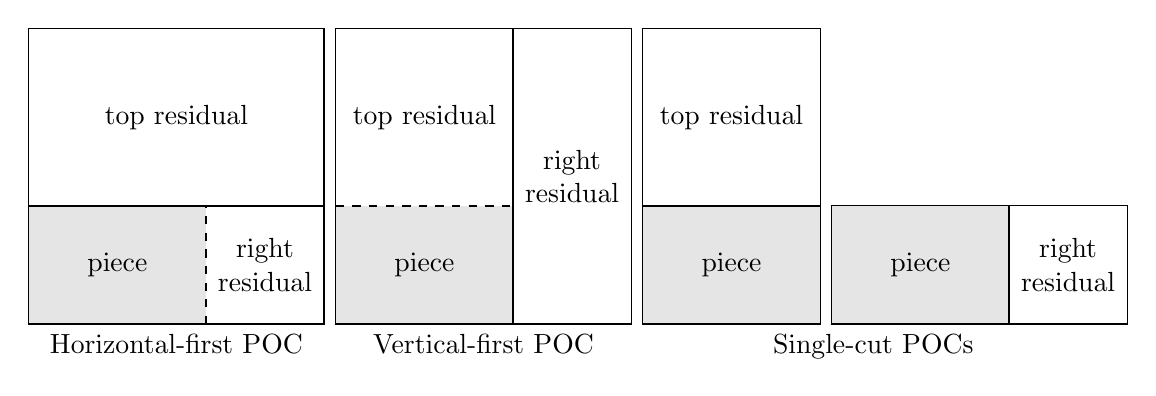
\begin{tikzpicture}[scale=0.15]
\def\piececolor{gray!20}
\def\labelxshift{12.5}
\def\labelyshift{0}
\def\labelfontsize{\normalsize}
\begin{scope}[shift={(0, 0)}] % FIRST ROW
\begin{scope}[shift={(0, 0)}] % FIRST IMAGE

\fill[\piececolor] (0, 0) rectangle +(15, 10);
\draw[thick, black] (0, 10) -- (25, 10);
\draw[dashed, thick, black] (15, 0) -- (15, 10);
\draw (0,0) rectangle +(25, 25);

\node [align=center, font=\labelfontsize\selectfont] at (7.5, 5) {\labelfontsize piece}; %{\labelfontsize piece-sized \\ \labelfontsize plate};
\node [align=center, font=\labelfontsize\selectfont] at (12.5, 17.5) {\labelfontsize top residual};
\node [align=center, font=\labelfontsize\selectfont] at (20, 5) {right\\residual};

\node [below] at (\labelxshift, \labelyshift) {\labelfontsize Horizontal-first POC};
\end{scope}

\begin{scope}[shift={(26, 0)}] % SECOND IMAGE

\fill[\piececolor] (0, 0) rectangle +(15, 10);
\draw[dashed, thick, black] (0, 10) -- (15, 10);
\draw[thick, black] (15, 0) -- (15, 25);
\draw (0,0) rectangle +(25, 25);

\node [align=center, font=\labelfontsize\selectfont] at (7.5, 5) {\labelfontsize piece}; %{\labelfontsize piece-sized \\ \labelfontsize plate};
\node [align=center, font=\labelfontsize\selectfont] at (7.5, 17.5) {\labelfontsize top residual};
\node [align=center, font=\labelfontsize\selectfont] at (20, 12.5) {right\\residual};

\node [below] at (\labelxshift, \labelyshift) {\labelfontsize Vertical-first POC};
\end{scope}

\begin{scope}[shift={(52, 0)}] % THIRD IMAGE

\fill[\piececolor] (0, 0) rectangle +(15, 10);
\draw[thick, black] (0, 10) -- (15, 10);
%\draw[dashed, thick, black] (15, 0) -- (15, 10);
\draw (0,0) rectangle +(15, 25);

\node [align=center, font=\labelfontsize\selectfont] at (7.5, 5) {\labelfontsize piece}; %{\labelfontsize piece-sized \\ \labelfontsize plate};
\node [align=center, font=\labelfontsize\selectfont] at (7.5, 17.5) {\labelfontsize top residual};
\end{scope}

\begin{scope}[shift={(68, 0)}] % FOURTH IMAGE

\fill[\piececolor] (0, 0) rectangle +(15, 10);
%\draw[dashed, thick, black] (0, 10) -- (15, 10);
\draw[thick, black] (15, 0) -- (15, 10);
\draw (0,0) rectangle +(25, 10);

\node [align=center, font=\labelfontsize\selectfont] at (7.5, 5) {\labelfontsize piece}; %{\labelfontsize piece-sized \\ \labelfontsize plate};
\node [align=center, font=\labelfontsize\selectfont] at (20, 5) {right\\residual};
\end{scope}
\node [below, align=center, font=\labelfontsize\selectfont] at (71.5, 0) {\labelfontsize Single-cut POCs};

\end{scope}
\end{tikzpicture}

  \legend{Souce: the author.}
  \label{fig:piece_outlining_cut}
\end{figure}

While a POC constituted by two BGCs may be considered as a single decision by a solving method and may be seen as happening in succession, in practice, stage restrictions may change the order a cutting machine perform them.
However, these real-world details do not impact our modelling and will not be discussed in this chapter.
Essentially, each piece type that fits into a plate has two POCs associated with it.
One POC that does the horizontal guillotine cut first and then obtains the piece from the first child plate through a vertical cut (if necessary).
This POC always leaves a \emph{top residual plate} (second child plate of the first cut) and often a \emph{right residual plate} (second child plate of the second cut).
The other POC is the same except that the vertical cut is done first (i.e., always leaving a right residual and often a top residual plate).
Finally, the piece-sized plate obtained by a POC is the first child plate of the second cut, if the second cut exists, otherwise just the first child plate of the only cut.
The piece-sized plate is either immediately regarded as an obtained piece (already enforcing a rule of the restricted problem), or it may be considered waste (e.g., the cutting stock problem often allow piece overproduction).
However, the piece-sized plate is \emph{never} treated as an intermediary plate that could be further cut.

A caveat of the coupled representation mentioned above is that, for some instances of the restricted problem, the number of POCs may be larger than the number of restricted cut positions.
In general, each piece type that fits into a plate has two POCs\footnote{The exception happens when the piece type shares the length or the width with the plate and, consequently, both POCs are equivalent and can be considered the same.} (vertical-first and horizontal-first).
A horizontal (vertical) BGC at a restricted position is shared by all piece types with the same length (width).
However, the main advantage of the coupled representation comes from breaking symmetries not reducing the number of variables.
%For example, if a stripe of width~\(10\) is obtained by a BGC in the restricted problem, it may be used to obtain a single piece of width~\(10\) and four pieces of width~\(8\), and every permutation in the order of the pieces are obtained from the strip is a symmetry, the POC enforce the width~\(10\) piece is the first to be obtained, and that no other mechanism is necessary to guarantee that the piece will be obtained from such plate.

The POCs are a natural choice for the \emph{restricted} problem but not for the \emph{unrestricted} problem for mostly two main reasons.
The first reason is that, in the restricted problem, each horizontal (vertical) cutting position shares length (width) with at least one piece.
However, in the unrestricted problem, some cutting positions can only be reached by combining many pieces.
The second reason is that the definition of the \emph{restricted} problem guarantees that employing only POCs cannot lead to optimality loss; the same is not true for the unrestricted problem (see \cref{fig:distinctions_restricted_unrestricted}).

\begin{figure}[h]
  \caption{Distinctions between, restricted, position-only restricted, and unrestricted problems.}
  \center
  \usetikzlibrary{patterns}
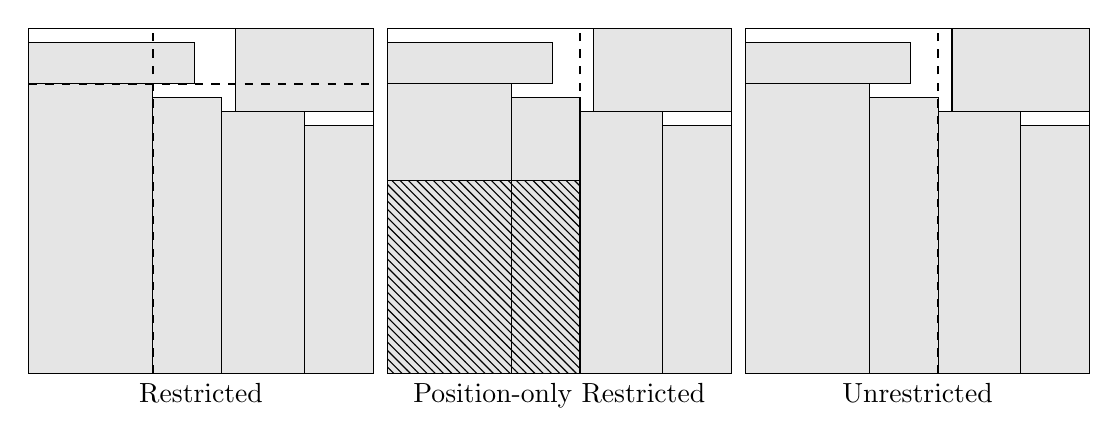
\begin{tikzpicture}[scale=0.175]
\def\piececolor{gray!20}
\def\labelxshift{12.5}
\def\labelyshift{0}
\def\labelfontsize{\normalsize}

\begin{scope}[shift={(0, 0)}] % FIRST ROW
\begin{scope}[shift={(0, 0)}] % FIRST IMAGE
\draw (0,0) rectangle +(25, 25);

%\draw[fill=\piececolor] (0,0) rectangle +(6, 19);
%\draw[fill=\piececolor] (6,0) rectangle +(5, 18);
\draw[fill=\piececolor] (14,0) rectangle +(6, 19);
\draw[fill=\piececolor] (20,0) rectangle +(5, 18);
\draw[fill=\piececolor] (0,0) rectangle +(9, 21);
\draw[fill=\piececolor] (9,0) rectangle +(5, 20);
%\draw[fill=\piececolor] (0,19) rectangle +(10, 6);
\draw[fill=\piececolor] (15,19) rectangle +(10, 6);
\draw[fill=\piececolor] (0,21) rectangle +(12, 3);

\draw[dashed, thick, black] (0, 21) -- (25, 21);
\draw[dashed, thick, black] (9, 0) -- (9, 25);


\node [below] at (\labelxshift, \labelyshift) {\labelfontsize Restricted};


\draw (0,0) rectangle +(25, 25);
\end{scope}

\begin{scope}[shift={(26, 0)}] % SECOND IMAGE
\draw (0,0) rectangle +(25, 25);

%\draw[fill=\piececolor] (0,0) rectangle +(6, 19);
%\draw[fill=\piececolor] (6,0) rectangle +(5, 18);
\draw[fill=\piececolor] (14,0) rectangle +(6, 19);
\draw[fill=\piececolor] (20,0) rectangle +(5, 18);
\draw[fill=\piececolor] (0,0) rectangle +(9, 21);
\draw[fill=\piececolor] (9,0) rectangle +(5, 20);
%\draw[fill=\piececolor] (0,19) rectangle +(10, 6);
\draw[fill=\piececolor] (15,19) rectangle +(10, 6);
\draw[fill=\piececolor] (0,21) rectangle +(12, 3);

\draw[pattern=north west lines] (0,0) rectangle +(14, 14);
\draw[dashed, thick, black] (14, 0) -- (14, 25);

\node [below] at (\labelxshift, \labelyshift) {\labelfontsize Position-only Restricted};
\end{scope}

\begin{scope}[shift={(52, 0)}] % THIRD IMAGE
\draw (0,0) rectangle +(25, 25);

%\draw[fill=\piececolor] (0,0) rectangle +(6, 19);
%\draw[fill=\piececolor] (6,0) rectangle +(5, 18);
\draw[fill=\piececolor] (14,0) rectangle +(6, 19);
\draw[fill=\piececolor] (20,0) rectangle +(5, 18);
\draw[fill=\piececolor] (0,0) rectangle +(9, 21);
\draw[fill=\piececolor] (9,0) rectangle +(5, 20);
%\draw[fill=\piececolor] (0,19) rectangle +(10, 6);
\draw[fill=\piececolor] (15,19) rectangle +(10, 6);
\draw[fill=\piececolor] (0,21) rectangle +(12, 3);

\draw[dashed, thick, black] (14, 0) -- (14, 25);

\node [below] at (\labelxshift, \labelyshift) {\labelfontsize Unrestricted};
\end{scope}

\end{scope}
\end{tikzpicture}

  \legend{The restricted problem cannot obtain the unrestricted optimal solution. If the first cut happens at a restricted position, the child plates cannot fit the six pieces of the optimal solution, regardless of the piece chosen to be obtained first from the original plate and the orientation of the first cut employed. The position-only restricted problem can obtain the unrestricted optimal solution if, by chance, there is an unpacked piece with a width that matches the necessary vertical cut; otherwise, the solution is also out of reach. Source: the author.}
  \label{fig:distinctions_restricted_unrestricted}
\end{figure}

\citet{silva:2010}~proposes a mathematical formulation for the two-stage and three-stage restricted cutting stock problems.
The formulation was not named by its authors; hence, in this text, it will be referred to as SAV (from the author's surname initials: Silva, Alvelos, and Valério).
The SAV is very similar to the FMT, which we examined in~\cref{sec:enhanced_model}.
In fact, the SAV may be seen as an FMT variant that uses POCs instead of BGCs.
The limitation to two- and three-stage problems comes from the cut and plate enumeration; this is, if the enumeration is not stopped at a specific stage, the SAV immediately supports unlimited stages.
Essentially, the proposed change is to: hybridise the FMT with the SAV, replacing BGCs by POCs \emph{only} when doing so cannot lead to loss of optimality for the unrestricted problem.
%Next section presents the implementation details for this change.

\section{Implementation details}

As seen in the last section, a POC (\emph{piece-oulining cut}) is prefered over a BGC (\emph{basic guillotine cut}) if it is guaranteed that replacing the latter by the former will not cause loss of optimality.
For the restricted problem, the typical set of horizontal (vertical) cutting positions is just the set of unique values in~\(l_i\) (\(w_i\)) for every piece type~\(i\) that fits into the plate.
Besides one corner case, each single guillotine cut at such positions may be replaced by the corresponding POC.
The corner case arises in cutting positions that come from a length (or width) value shared by two or more pieces.
In this case, a single guillotine cut needs to be replaced by two or more POCs, depending on how many pieces share the corresponding cutting position; otherwise, the model would lose the capability to produce that piece type.

For the unrestricted problem, the exact set of cutting positions often vary between different solving methods.
There are many discretization procedures (see \cref{sec:enhanced_model}) and reductions to be applied either after or during such discretizations.
The author will focus on the discretizations and reductions procedures employed by the formulations of~\cref{sec:furini_vs_enhanced_comparison} (this is, the FMT and BBA formulations).
The base discretization employed by both FMT and BBA is straightforward: \(q\) is a horizontal (vertical) cutting position if, and only if, there is a demand-abiding linear combination of lengths (widths) from pieces that fit into the respective plate.
This cutting position set is a superset of the restricted set (from the last paragraph) and will be referred to as the \emph{base unrestricted set}.
Suppose a cutting position allows for the associated BGC to be replaced by (one or more) POCs without loss of optimality for the \emph{unrestricted problem}.
In that case, the cutting position (and by extension the BGC) is said to be \emph{replaceable}.
%The set of cutting positions for which the associated single guillotine cuts may be replaced by POCs, without loss of optimality in the context of the \emph{unrestricted problem}, will be referred to as the \emph{replaceable set} henceforth.

A cutting position must meet two conditions to be deemed replaceable.
The first condition is that a cutting position of the same orientation for the same plate exists in the restricted set.
The second condition is that such horizontal (vertical) cutting positions cannot be obtainable by a demand-abiding linear combination of two or more piece lengths (widths), taking into account only the pieces that fit into the respective plate.
The first condition is necessary because, otherwise, the cut is not outlining a piece, i.e., there is no corresponding piece type to be extracted from the first child plate.
The second condition is necessary because, otherwise, the replaced cut could be necessary for the only optimal cutting pattern of an instance of the unrestricted problem, as it is shown in~\cref{fig:distinctions_restricted_unrestricted}.
%the sum of lengths (widths) for a piece multiset in which (a) each piece type multiplity respects the demand, (b) each piece type fits into the first child plate, and (c) the multiset has a cardinality of two or more.
% NOTE: probably we need an image with three diagrams, two of them equal to the introduction ones and a third image showing the possibility of the cut if there is an out-of-the-pattern piece type that has the same size as two other summed.

The two reductions proposed in~\cite{furini:2016}, \emph{Cut-Position} and \emph{Redundant-Cut}, cause little change to the replaceable cutting positions.
If a plate cannot pack six or more pieces, then its restricted and unrestricted optimal value is the same (see \cref{fig:distinctions_restricted_unrestricted}), and \emph{Cut-Position} reduce the set of cutting positions over such plate to the restricted set.
The only cutting positions removed by \emph{Cut-Position} are, therefore, the ones not in the restricted set and, therefore, not replaceable.
Moreover, if the cutting position set of a plate is reduced by \emph{Cut-Position} and the kept positions are all replaced with POCs, then that plate and any plate strictly smaller than it will, in fact, be solved by the SAV formulation instead of the FMT formulation.

The \emph{Redundant-Cut} reduction only removes \emph{trim cuts}, i.e., cuts in which the second child plate is immediately considered waste because no piece can fit into it.
\emph{Redundant-Cut} removes a trim cut over plate~\(j\), which obtains plate~\(j^\prime\), if plate~\(j\) itself can \emph{only} be obtained by trim cuts of the same orientation from larger plates. The rationale is that these larger plates can directly obtain~\(j^\prime\) and avoid the many symmetric patterns that are only distinguished by the number of trim cuts employed to reduce a plate to a smaller size.
\emph{Redundant-Cut} may remove a replaceable cutting position. However, the predicted alternative cutting position from a larger plate will always be replaceable too, and replacing it with one or more POCs never requires we add back the cuts removed by Redundant-Cut.
Also, the BBA formulation never has trim cuts (see \cref{sec:enhanced_model}), so this enhancement is superseded by it.

BBA adds extraction variables and reduces the base unrestricted set to only the cutting positions up to the midplate.
The extraction variables can be seen as POCs in which both top and right residual plates are guaranteed to be waste and, therefore, extractions are not subject to be replaced by POCs themselves.
BBA requires us to differentiate between \emph{binding} and \emph{non-binding} POCs.
A POC is \emph{non-binding} if the piece-sized plate it obtains may be regarded as waste; conversely, if the piece-sized plate must be sold as a piece, then the POC is \emph{binding}.
A \emph{binding} POC cannot be employed if an extra copy of the associated piece type would lead to disrespecting the demand constraint.
If replaceable cuts in the BBA formulation are replaced by \emph{binding} POCs, then there are cases in which loss of optimality occurs.
The cause of this loss of optimality is that, in BBA, a replaceable cut may be required by an optimal solution even if there is no demand for the associated piece.
The goal of these seemingly unnecessary cuts is to reduce the size of a plate until a large piece can be obtained from the plate through an extraction variable.
A complete example follows.

\begin{example}{Hybridised BBA with binding cuts loses optimality.}
Consider the following G2KP instance: \(L = 100\), \(W = 100\), \(l = [100, 100]\), \(w = [1, 51]\), \(d = [1, 1]\), and \(p = [1, 1]\).
The optimal solution clearly must contain the only available copy of each of the two piece types.
In BBA, there is no cut after the midplate, and, consequently, a vertical cut at position \(51\) is ruled out.
The only possibility is a vertical cut at position \(1\) for which the first child plate could be immediately sold as the single copy of the first piece type.
The second child plate (\(100\)x\(99\)) also does not have an extraction variable for the immediate extraction of the second piece type (\(100\)x\(51\)).
The BBA determines that for an extraction variable to exist ``[...] the plate cannot fit an extra piece (of any type).'' and the first piece type fits together with the second in the \(100\)x\(99\) plate.
Again, a vertical cut at position \(51\) is unavailable because it happens after midplate.
Consequently, BBA forces the optimal solution to create \(50\) plates of size \(100\)x\(1\), one which will be sold as a piece, and the rest considered waste.
The second child of the \(50\)th (and last) cut has size \(100\)x\(50\), and it can be sold as the second piece type because an extraction variable is now available (i.e., the previously quoted condition does not apply anymore).
The adoption of \emph{binding} POCs makes it impossible for BBA to obtain an optimal solution for this example.
The reason is that there are not \(50\) copies of the first piece type, but these would be needed by the \(50\) binding piece-outlining cuts necessary to obtain an optimal solution.
The same problem does not arise if the POCs are not binding.
\end{example}

The corner case of two or more pieces sharing the same length/width needs to be considered in the unrestricted problem too, but with a subtle distinction.
In the restricted problem, replacing every single guillotine cut by POCs also brings the advantage of not needing an additional mechanism to enforce the problem definition (i.e., to guarantee piece extractions from the first child plates).
However, in the unrestricted problem, the choice between replacing a single guillotine cut by multiple POCs, or keeping it as a guillotine cut, is just a trade-off between model size and model symmetry.
Therefore, we further distinguish between two implementations of hybridisation.
The \emph{conservative} hybridisation substitutes each replaceable horizontal (vertical) BGC by one horizontal-first (vertical-first) POC associated to the single piece type that matches the length (width) of the cutting position (and that fits into the respective plate); if two or more fitting piece types match the cutting position then the conservative hybridisation leaves the BGC unchanged.
The \emph{aggressive} hybridisation substitutes each replaceable horizontal (vertical) BGC by one horizontal-first (vertical-first) POC for each piece type that matches its length (width) (and that fits into the respective plate).
%enhancement based on how they deal with the corner case of multiple pieces sharing length or width.
%The distinction between aggressive and conservative is made mostly during cut and plate enumeration, and depending on implementation details, the model formulation may be kept blind to it, i.e., only taking into account which cuts are BGCs and which are POCs.

The author believes it is excessive to present the full formulation and implementation details for every combination of the FMT/BBA formulation with conservative/aggressive hybridisation and binding/non-binding POCs.The experiments in the next section only consider the BBA with conservative/aggressive hybridisation and non-binding POCs.
The distinction between conservative and aggressive hybridisation is mostly made at the cut and plate enumeration; however, because of an unfortunate notation detail explained further, it is less troublesome to present an accurate formulation of the conservative hybridisation than the aggressive hybridisation.
In light of this, the author chose to fully present the conservative hybridised BBA formulation with non-binding POCs.
The main differences in implementing other combinations are briefly discussed shortly after.

The \emph{conservative hybridised BBA formulation with non-binding} POCs requires a new set of variables, a new set of constraints, a new parameter, and some minor changes to the objective function and some of the existing constraints.
Both the new set of variables and the new set of constraints are bounded by \(|\bar{J}|\) and, therefore, they cause only a small relative increase to the model size of a non-trivial instance.
The notation for the new variable and parameter set follows:

\begin{description}
\item [\(s_i\)] \(\forall i \in \bar{J}\) -- Integer variable. Indicates how many piece-sized plates obtained by POCs associated with piece type~\(i\) were sold as pieces of type~\(i\). By \emph{sold} the author means they contributed to the objective function and were accounted for by the demand constraint.
\item [\(h^o_{qji}\)] \(\forall o \in O, j \in J, q \in Q_{jo}, i \in \bar{J}\) -- Binary parameter. Byproduct of the cut and plate enumeration. One if cut~\(x^o_{qj}\) produces a piece-sized plate corresponding to piece~\(i\); zero otherwise. For a cut~\(x^o_{qj}\), \(\sum_{i\in\bar{J}} h^o_{qji}\) is zero if the cut is a BGC, and one if the cut is a POC.
\end{description}

Some variables, parameters, and constraints need just a little reinterpretation or no change at all.
The already established parameter \(a^o_{qkj}\) is exactly the same for BGCs and has a slightly different meaning for POCs.
The difference is that the \(j\) (obtained child plate) is always either the top or right residual (i.e., the POC version of the first and second child) and that both \(o\) (orientation) and \(q\) (cutting position) refer only to the first constituting cut of a POC; the meaning of \(k\) (parent plate) is left unchanged.
The set of variables representing cuts (\(x^o_{qj}\)) also does not need change, as \(h^o_{qji}\) fills the need to identify POCs and their associated piece types.Consequently, the constraints~\eqref{eq:plates_conservation,eq:just_one_original_plate} presented below are the same as the non-hybridised formulation.

The constraint~\eqref{eq:piece_sized_plates} guarantees each piece-sized plate available~(\(s_i\)) comes from an actual POC.
The remaining changes consist into adding \(s_i\) to the demand constraint~\eqref{eq:hyb_demand} (which avoids overproduction without prohibiting the POCs themselves) and to the objective function~\eqref{eq:hyb_obj} (which allows piece-sized plates to be sold).

% TODO: check if labels are correct

\begin{align}
\bm{max.} &\sum_{(i, j) \in E} p_i e_{ij} + \sum_{i \in \bar{J}} p_i s_i \label{eq:hyb_obj}\\
\bm{s.t.} &\specialcell{\sum_{o \in O}\sum_{q \in Q_{jo}} x^o_{qj} + \sum_{i \in E_{*j}} e_{ij} \leq \sum_{k \in J}\sum_{o \in O}\sum_{q \in Q_{ko}} a^o_{qkj} x^o_{qk} \hspace*{0.05\textwidth} \forall j \in J, j \neq 0,}\tag{\ref{eq:plates_conservation}}\\
	    & \specialcell{\sum_{o \in O}\sum_{q \in Q_{0o}} x^o_{q0} + \sum_{i \in E_{*0}} e_{i0} \leq 1 \hspace*{\fill},}\tag{\ref{eq:just_one_original_plate}}\\
            & \specialcell{s_i \leq \sum_{j \in J}\sum_{o \in O}\sum_{q \in Q_{jo}} h^o_{qji} x^o_{qj} \hspace*{\fill} \forall i \in \bar{J},}\label{eq:piece_sized_plates}\\%\tag{\ref{eq:piece_sized_plates}}\\
            & \specialcell{s_i + \sum_{j \in E_{i*}} e_{ij} \leq u_i \hspace*{\fill} \forall i \in \bar{J},}\label{eq:hyb_demand}\\
	    & \specialcell{x^o_{qj} \in \mathbb{N}^0 \hspace*{\fill} \forall j \in J, o \in O, q \in Q_{jo},}\tag{\ref{eq:trivial_x}}\\
            & \specialcell{e_{ij} \in \mathbb{N}^0 \hspace*{\fill} \forall (i, j) \in E}\tag{\ref{eq:trivial_e}}\\
            & \specialcell{s_{i} \in \mathbb{N}^0 \hspace*{\fill} \forall i \in \bar{J}.}\label{eq:trivial_s}
\end{align}

The aforementioned unfortunate notation detail is the incapability of denoting two or more different cuts~(\(x^o_{qj}\) with same orientation~\(o\) and cutting position~\(q\) over the same plate~\(j\).
Therefore, if the aggressive hybridisation replaces a BGC with two or more POCs, then the notation does not allow us to differentiate between them.The~\(a^o_{qkj}\) parameter also needs to change, as it suffers from the same problem.
The aggressive hybridisation code deals with this problem by having unique single indexes for each cut and reverse indexes from each cut property (like orientation or cutting position) to the cuts themselves; this way, the cuts are not limited to the uniqueness of some property combination.

% THE COMMENTED TEXT BELOW IS BETWEEN WRONG AND UNNECESSARY, the problem of using the parameter 'a' the current way is that every POC that shares a BGC will generate all piece-sized plates instead, but badly trying to fix could have lead to the problem mentioned below.
%Even just replacing~\(x^o_{qj}\) is not enough, because  can represent most different POCs originated from the same BGC, because the \(j\), except for one exception.
%The exception is the existence of two or more piece types with the exact same dimensions but distinct profits.
%However, the author chose to not complicate the formulation just to encompass this rare corner case.
%The complication exists because of the \(a^o_{qkj}\) notation does not foresee the need of two distinct cuts in the same plate at the same cutting position with the same orientation and that obtain the same children plates.

A trivial way to change the presented formulation to use \emph{binding cuts} is to change constraint~\eqref{eq:piece_sized_plates} to require equality.
However, the binding cuts can also be implemented without the new variable and constraint sets.
The term \(s_i\) could just be replaced by \(\sum_{j \in J}\sum_{o \in O}\sum_{q \in Q_{jo}} h^o_{qji} x^o_{qj}\) in both the objective function and the demand constraint.
Both mentioned ways to implement binding cuts work on the FMT formulation, which does not have the same loss of optimality problem as the BBA.

% FROM FURINI 2016 PAGE 8: "As an example, if there are three items with widths 21 31 5, the Restricted PP-G2KP Model would allow us to cut at position q = 5 and then perform a further cut at position q = 2 on the obtained plate. Hence, the width of the strip obtained by cutting at position 5 would not correspond to the width of one of the obtained items. For this reason, the Restricted PP-G2KP Model can produce solutions that do not satisfy the definition of restricted guillo- tine cuts given in Section 1."

\section{Experimental results}

In these experiments, for reasons explained further ahead, each instance was solved ten times with ten distinct solver seeds.
The BBA configuration included all applicable reductions previously discussed (i.e., Cut-Position and Plate-Size Normalization) but excluded initialization with a primal heuristic and pricing.
The barrier algorithm was used to solve the root node as usual.
Only the Gurobi solver is used in these experiments.No runs ended in timeout.
Three variants are scrutinized: no hybridisation (N. H.), conservative hybridisation (C. H., avoids increasing model size), and aggressive hybridisation (A. H., always hybridise, even if it leads to an increase of the model size).

\Cref{tab:g2kp_hyb_summary} shows that both C. H. and A. H. had a similar impact on the total solving time (i.e., a reduction of \(\approx\)20\%).
A. H. had slightly better timings despite the considerable increase in the number of cuts.
C. H. slightly reduces the number of cuts.
Both C. H. and A. H. have almost no effect on the number of plates (or extractions variables).
The percentage of hybridised cuts (\emph{h \%}) and hybridised cuts with just one residual (\emph{k \%}) show that the new reductions changed a very significant part of the models.
The number of instances with the lowest averages shows that N. H. is the best option for most instances.

\begin{table}
\caption{Summary of hybridisation impact over BBA formulation and FMT59 dataset.}
\label{tab:g2kp_hyb_summary}
\begin{center}

\begin{tabular}{lrrrrrrrr}
\hline\hline
\textbf{Variant} & \textbf{T. T.} & \textbf{T. L.} & \textbf{\#b} & \textbf{\#extr.} & \textbf{\#cuts} & \textbf{h \%} & \textbf{k \%} & \textbf{\#plates} \\\hline
N. H. & 6,681 & 1,703 & 27 & 186,536 & 2,498,801 & -- & -- & 113,822 \\
C. H. & 5,468 & 489 & 22 & 184,067 & 2,496,421 & 41 & 18 & 113,373 \\
A. H. & 5,447 & 469 & 10 & 184,050 & 3,021,911 & 67 & 28 & 113,366 \\\hline\hline
\end{tabular}
\end{center}

\legend{\emph{T. T.} (Total Time) -- sum of the mean time of all instances, in seconds; \emph{T. L.} (Time Loss) -- sum of the difference in mean time between the respective variant and the variant with the lowest mean time for the same instance, in seconds, i.e., if all variants ran in parallel and had average time, how much time the runs of the respective variant would spend after another thread already finished; \emph{\#b} (best) -- number of instances in which the respective variant had the lowest (best) average time among the variants; \emph{\#extr.} -- total number of extraction variables (considering one model per instance); \emph{\#cuts.} -- total number of cut variables (considering one model per instance); \emph{h \%} -- percentage of \#cuts that were hybridised; \emph{k \%} -- percentage of \#cuts that were not only hybridised but also discarded the second child of the second constituting cut as waste, i.e., the POC resulted in the piece-sized plate and \emph{one} other plate; \emph{\#plates} -- total number of plates (considering one model per instance). Source: the author.}
\end{table}

A closer look into the data, see \Cref{tab:g2kp_hyb_selected_instances}, reveals that most time difference comes from a few hard instances.
In fact, the instance Hchl4s alone is responsible for most of the difference, with okp2 having about half its relevance and the rest of the instances considerably less impact.
The number of variables hybridised (\emph{H} columns) does not seem a good indicator of how impacted the solving times will be.
However, if N. H. spends most of the time solving the root node (low Non-Root \%), C. H. and A. H. generally do not bring great time improvements.
As the most significant reductions often occur in instances that spend less than 1\% of the time in the root node, the time distribution does not change significantly.
An exception is CHL1s which shows that C. H. seems to impact not the time at the root node but the time at the B\&B, as expected from a symmetry breaking enhancement.

\begin{table}
\caption{Impact of BBA hybridisation in FMT59 instances taking more than 10s.}
\label{tab:g2kp_hyb_selected_instances}
\begin{center}
%\resizebox{!}{.77\height}{%
\begin{tabular}{lrrrrrrrrrrr}
\hline\hline
& \multicolumn{2}{c}{H (\%)} & \multicolumn{3}{c}{Mean} & \multicolumn{3}{c}{CV (\%)} & \multicolumn{3}{c}{Non-Root (\%)} \\\cmidrule(lr){2-3}\cmidrule(lr){4-6}\cmidrule(lr){7-9}\cmidrule(lr){10-12}
Inst. & C & A & N (s) & C (\%) & A (\%) & N & C & A & N & C & A \\\hline\hline
Hchl4s & 46 & 57 & 3,657 & 80 & \bestcolumnemph{69} & 76 & 35 & 25 & >99 & >99 & >99 \\
okp2 & 22 & 22 & 1,844 & \bestcolumnemph{77} & 88 & 21 & 19 & 44 & >99 & >99 & >99 \\
Hchl7s & 50 & 77 & 428 & \bestcolumnemph{100} & 134 & 18 & 26 & 19 & 25 & 36 & 44 \\
okp3 & 33 & 49 & \bestcolumnemph{209} & 113 & 122 & 29 & 38 & 35 & >99 & >99 & >99 \\
Hchl8s & 17 & 35 & 253 & 68 & \bestcolumnemph{48} & 73 & 45 & 44 & >99 & >99 & >99 \\
Hchl3s & 46 & 57 & 39 & \bestcolumnemph{93} & 130 & 11 & 21 & 85 & 80 & 82 & 87 \\
Hchl2 & 25 & 77 & 45 & \bestcolumnemph{89} & 144 & 5 & 8 & 18 & 49 & 50 & 65 \\
CHL6 & 45 & 68 & 39 & \bestcolumnemph{91} & 98 & 13 & 15 & 14 & 48 & 46 & 44 \\
CHL7 & 23 & 78 & \bestcolumnemph{30} & 105 & 116 & 8 & 8 & 5 & 26 & 27 & 44 \\
Hchl6s & 51 & 80 & \bestcolumnemph{36} & 103 & 103 & 3 & 5 & 3 & 14 & 18 & 27 \\
CHL1 & 32 & 64 & \bestcolumnemph{26} & 115 & 120 & 14 & 16 & 14 & 68 & 71 & 72 \\
CHL1s & 32 & 64 & 21 & \bestcolumnemph{75} & 121 & 14 & 13 & 6 & 62 & 39 & 61 \\
okp5 & 11 & 12 & 12 & \bestcolumnemph{97} & 99 & 1 & 2 & 2 & 19 & 21 & 21 \\\hline\hline
\end{tabular}
%} % resizebox
\end{center}
\legend{\emph{H (\%)} -- percentage of all variables (i.e., cut and extraction) that were hybridised for C. H. and A. H.; \emph{Mean} -- mean time spent to solve the instance, in seconds for N. H., and in a percentage relative to N. H. for both C. H. and A. H.; \emph{CV} -- coefficient of variation (also known as relative standard deviation) is the standard deviation for N. H., C. H., and A. H., divided by their respective means (CV is always a percentage); \emph{Non-Root (\%)}} -- percentage of the total time which was \emph{not} spent solving the root node. Source: the author.
\end{table}

The coefficient of variation of the analysed instances reveals the reason for multiple runs with distinct seeds: the difference between two runs of the same variant but distinct seeds is often larger than the difference between the means of two distinct variants.
Intuitively, breaking symmetries should reduce the variance of the timings.
By cutting symmetric branches, there is less opportunity for a solver seed to traverse multiple equivalent branches with a good relaxation (but bad primal) before finding a primal solution that cuts all such branches.
In fact, when C. H. and A. H. achieve a considerable (20\% or more) reduction of the mean time, the coefficient of variation (which is relative to the mean time) generally shows reduction.
However, a more general effect, i.e., a higher percentage of model hybridisation (H \%) leading to lower CV (or mean time), is not observed.
Exactly which variables were hybridised probably have more impact than how many.
Finally, the reduction of variance, while positive if the objective is to compare solution methods, may be unwanted when solving the same problem in parallel.
For example, if two methods have similar mean times, the method with the most variance will probably have a thread find the optimal solution first.

The Clautiaux42 dataset has two traits that make it a worst-case scenario for both C. H. and A. H.: most instances are small instances, and the number of pieces sharing the same length, or width, is high.
For the sake of comparison, let us define \(rr_l\) (\(rr_w\)) as the \emph{repeat ratio} of the length (width) values of pieces.
For a given set of piece types, the \(rr_l\) (\(rr_w\)) is a fraction with the difference between the set cardinality and the number of distinct length (width) values as the numerator, and the set cardinality minus one as the denominator.
\emph{Zero} means there is no repetition, and \emph{one} means that all pieces share the same value in the respective dimension.
The FMT59 dataset has \(rr_l \approx 0.178\) and \(rr_w \approx 0.155\), while the Clautiaux42 has \(rr_l \approx 0.465\) and \(rr_w \approx 0.402\).
The metric is a good baseline, even if it does not account for some important details.
For example, small piece types sharing a small length, or width, cause more hybridisation than large pieces sharing a large length (or width).
This last observation is especially true for the BBA formulation, which has no cuts after the midplate.

\Cref{tab:g2opp_hyb_summary} shows that C. H. hybridises only \(\approx\)5\% of the variables and has minimal impact, while A. H. hybridises \(\approx\)55\% of the variables but cause a large increase in both time to solve and the number of cut variables.
\Cref{tab:g2opp_hyb_summary} reveals that for many instances, C. H. has less than 0.5\% of hybridised variables, and the mean and CV show they behave basically the same as N. H. for most instances.
In fact, the slight advantage of C. H. comes from the fact that the two hardest instances have no hybridisation and, therefore, the same mean time as N. H.
But the third-hardest instance reaps a few seconds from the hybridisation of 9\% of the variables.
The extra variables from the A. H. have a very strong negative effect on the mean time for all instances.
For some instances (as E05F18 and E00X23), the mean time is more than ten times longer than N. H.
Finally, if rotation is allowed, then \(rr_l\) and \(rr_w\) become a single metric that can only be greater than or equal to both previous values; consequently, the gap in behaviour between C. H. and A. H. can only increase by allowing rotation.

\begin{table}
\caption{Summary of hybridisation impact over BBA formulation and Clautiaux42 dataset.}
\label{tab:g2opp_hyb_summary}
\begin{center}
\begin{tabular}{lrrrrrrrr}
\hline\hline
\textbf{Variant} & \textbf{T. T.} & \textbf{T. L.} & \textbf{\#b} & \textbf{\#extr.} &\textbf{\#cuts} & \textbf{h \%} & \textbf{k \%} & \textbf{\#plates} \\\hline
N. H. & 255.10 & 11.30 & 32 & 1,205 & 109,369 & 0.00 & 0.00 & 12,642 \\
C. H. & 251.58 & 7.78 & 10 & 1,205 & 109,369 & 5.50 & 2.11 & 12,642 \\
A. H. & 858.30 & 614.50 & 0 & 1,205 & 160,650 & 55.23 & 10.78 & 12,642 \\\hline\hline
\end{tabular}
\end{center}
\legend{The description of the columns can be found in~\Cref{tab:g2kp_hyb_summary}. Source: the author.}
\end{table}

In general, for both datasets, C. H. did either have a negligible difference from N. H. or did provide some considerable benefit (especially for instances with longer running times).
For solving mostly small instances, or instances with high \(rr_l\) or \(rr_w\), the extra complexity brought to the formulation may not be worthwhile, but the change does not bring much risk of worsening the results.
The A. H. has the best reduction of mean time and CV for both Hchl4s and Hchl8s (FMT59 dataset), but it has a consistently terrible performance for small instances with high \(rr_l\) and \(rr_w\).
There is no clear class of instances for which it can consistently outperform C. H. (or N. H.).

\begin{table}
\caption{Details of hybridisation impact over BBA formulation and Clautiaux42 dataset.}
\label{tab:g2opp_multiple_seeds_full_CV_hyb}
\begin{center}
%\resizebox{!}{.77\height}{%
\begin{tabular}{lrrrrrrrrrrr}
\hline\hline
& \multicolumn{2}{c}{H (\%)} & \multicolumn{3}{c}{Mean} & \multicolumn{3}{c}{CV (\%)} & \multicolumn{3}{c}{Non-Root (\%)} \\\cmidrule(lr){2-3}\cmidrule(lr){4-6}\cmidrule(lr){7-9}\cmidrule(lr){10-12}
Inst. & C & A & N (s) & C (\%) & A (\%) & N & C & A & N & C & A \\\hline\hline
E02F20 & 0 & 58 & \bestcolumnemph{83.70} & 100 & 350 & 62 & 62 & 70 & >99 & >99 & >99 \\
E20F15 & 0 & 54 & \bestcolumnemph{68.26} & 101 & 212 & 51 & 49 & 67 & >99 & >99 & >99 \\
E04F19 & 9 & 57 & 26.59 & \bestcolumnemph{64} & 183 & 117 & 118 & 156 & >99 & >99 & >99 \\
E05F18 & 0 & 57 & \bestcolumnemph{8.52} & 111 & 1,172 & 21 & 17 & 51 & >99 & >99 & >99 \\
E10X15 & 15 & 55 & \bestcolumnemph{7.62} & 124 & 292 & 64 & 28 & 96 & 99 & >99 & >99 \\
E08F15 & 0 & 51 & \bestcolumnemph{5.05} & 115 & 424 & 34 & 33 & 63 & 99 & 99 & >99 \\
E04F17 & 0 & 54 & \bestcolumnemph{4.50} & 100 & 730 & 16 & 16 & 7 & 99 & 99 & >99 \\
E02N20 & 0 & 55 & \bestcolumnemph{4.23} & 100 & 721 & 17 & 17 & 45 & 99 & 99 & >99 \\
E05X15 & 9 & 51 & 3.46 & \bestcolumnemph{92} & 213 & 25 & 25 & 31 & 99 & 99 & 99 \\
E02F17 & 2 & 54 & \bestcolumnemph{3.43} & 111 & 239 & 26 & 17 & 20 & 99 & 99 & >99 \\
E07F15 & 2 & 59 & \bestcolumnemph{3.27} & 121 & 418 & 23 & 28 & 26 & 99 & 99 & >99 \\
E04F20 & 2 & 53 & 2.95 & \bestcolumnemph{76} & 469 & 53 & 43 & 145 & 99 & 98 & >99 \\
E15N15 & 12 & 55 & \bestcolumnemph{2.78} & 123 & 159 & 83 & 77 & 87 & 99 & 99 & 99 \\
E07X15 & 0 & 51 & 2.55 & \bestcolumnemph{99} & 300 & 17 & 18 & 45 & 99 & 98 & 99 \\
E00X23 & 0 & 55 & \bestcolumnemph{2.26} & 100 & 1,237 & 11 & 11 & 100 & 97 & 97 & >99 \\
E03X18 & 0 & 56 & 2.26 & \bestcolumnemph{86} & 310 & 28 & 19 & 40 & 98 & 97 & 99 \\
E04N17 & 9 & 49 & \bestcolumnemph{1.99} & 128 & 234 & 40 & 35 & 31 & 98 & 98 & 99 \\
E03N17 & 2 & 57 & \bestcolumnemph{1.98} & 115 & 236 & 13 & 10 & 18 & 98 & 98 & 99 \\
E04F15 & 1 & 49 & \bestcolumnemph{1.94} & 101 & 182 & 14 & 9 & 13 & 98 & 98 & 99 \\
E03N16 & 1 & 55 & \bestcolumnemph{1.78} & 110 & 337 & 21 & 12 & 19 & 98 & 98 & 99 \\
E02F22 & 4 & 54 & \bestcolumnemph{1.72} & 101 & 321 & 41 & 38 & 55 & 98 & 98 & 99 \\
E04N18 & 0 & 55 & 1.62 & \bestcolumnemph{86} & 743 & 32 & 25 & 48 & 98 & 98 & >99 \\
E05F20 & 10 & 55 & \bestcolumnemph{1.36} & 113 & 243 & 33 & 41 & 45 & 97 & 97 & 98 \\
E00N23 & 0 & 49 & 1.33 & \bestcolumnemph{96} & 215 & 12 & 15 & 22 & 96 & 96 & 98 \\
E08N15 & 8 & 61 & \bestcolumnemph{1.19} & 106 & 436 & 18 & 15 & 29 & 97 & 98 & 99 \\
E05N17 & 0 & 53 & \bestcolumnemph{1.17} & 112 & 364 & 18 & 15 & 52 & 97 & 97 & 99 \\
E05F15 & 11 & 53 & \bestcolumnemph{1.10} & 107 & 386 & 9 & 15 & 24 & 96 & 97 & 99 \\
E15N10 & 13 & 53 & 1.09 & \bestcolumnemph{88} & 236 & 20 & 30 & 24 & 97 & 97 & 98 \\
E03N15 & 9 & 61 & \bestcolumnemph{1.09} & 109 & 249 & 10 & 10 & 22 & 96 & 97 & 98 \\
E05N15 & 1 & 55 & \bestcolumnemph{0.72} & 113 & 200 & 33 & 15 & 21 & 96 & 95 & 97 \\
E20X15 & 0 & 55 & \bestcolumnemph{0.71} & 105 & 531 & 25 & 25 & 45 & 94 & 95 & 99 \\
E07N15 & 8 & 63 & \bestcolumnemph{0.58} & 116 & 313 & 44 & 46 & 105 & 97 & 97 & 98 \\
E04N15 & 19 & 57 & \bestcolumnemph{0.48} & 111 & 350 & 12 & 13 & 20 & 93 & 94 & 97 \\
E13X15 & 0 & 57 & 0.48 & \bestcolumnemph{93} & 205 & 19 & 18 & 19 & 94 & 91 & 96 \\
E13N10 & 13 & 52 & \bestcolumnemph{0.37} & 112 & 164 & 13 & 18 & 14 & 92 & 93 & 95 \\
E00N15 & 1 & 53 & \bestcolumnemph{0.25} & 104 & 134 & 8 & 8 & 11 & 76 & 77 & 83 \\
E13N15 & 5 & 56 & \bestcolumnemph{0.24} & 113 & 787 & 8 & 10 & 25 & 84 & 85 & 97 \\
E07N10 & 32 & 59 & \bestcolumnemph{0.16} & 119 & 158 & 37 & 22 & 13 & 87 & 89 & 88 \\
E10N10 & 21 & 62 & \bestcolumnemph{0.14} & 117 & 218 & 44 & 38 & 15 & 86 & 83 & 90 \\
E10N15 & 29 & 52 & \bestcolumnemph{0.08} & 117 & 148 & 11 & 9 & 8 & 66 & 67 & 73 \\
E03N10 & 11 & 51 & 0.08 & \bestcolumnemph{95} & 166 & 9 & 6 & 8 & 34 & 28 & 76 \\
E00N10 & 31 & 61 & \bestcolumnemph{0.04} & 132 & 199 & 4 & 2 & 109 & 15 & 22 & 61 \\\hline\hline
\end{tabular}
%} % resizebox
\end{center}
\legend{The description of the columns can be found in~\Cref{tab:g2kp_hyb_selected_instances}. Source: the author.}
\end{table}


\chapter{About the T instances from \protect\citethopperthesis}
\label{sec:about_T_instances}

In a preliminary experiments phase, the author considered the instances of the datasets N and T from \citet{hopper_thesis}. % Eva Hopper's Thesis~
Each dataset has 35 instances, and was generated by recursively cutting a 200x200 plate. %See more on %The number of instances (35) comes from 7 distinct \(n\) values (17, 25, 29, 49, 73, 97, 199) times 5 random seeds.

%In \citet{hopper_thesis}, the instances were used to evaluate heuristics for the Strip Packing Problem.
%The instances have a width of 200 and their optimal length is 200 (a pattern with no waste).
%Hence, the optimality gap could be easily computed.

\citet{hopper_thesis} distinguishes between N and T solely by the cutting rules employed to generate each dataset.
In N, a plate randomly selected to be further cut is divided into five subplates which follow the classic non-guillotinable pattern (see the pieces 12, 13, 14, 15, and 16 in \Cref{fig:T1a} for an example of such pattern).
In T, single (vertical or horizontal) guillotine cuts should have been used instead.
When the number of plates reaches a desired number, the process stops, and each plate is considered a piece for the generated instance.
The process discards no plate and, therefore, an optimal solution that packs every piece into a 200x200 plate must exist.
However, only the process described for the T instances guarantee that optimal solutions can be obtained by using only guillotine cuts.

\begin{comment}
Instances for which we proved infeasibility:
jl_yMhj5m T1a
jl_meyQRn T1b
jl_IJhWMm T1c
jl_aGVVYp T1d
jl_on4aRl T1e
jl_axD9ro T2c
jl_idk5Cm T2e
jl_61BNyp T3a
\end{comment}

%In our preliminary experiments, we  by adopting \(L = 200\), \(W = 200\), and \(p_i = 1, \forall i \in 1..n\).
Even with a three hours time limit we optimally solved only 8 instances of dataset T (T1a, T1b, T1c, T1d, T1e, T2c, T2e, T3a).
However, in each of these 8 runs, the solver returned an optimal pattern with less than all pieces of the respective instance.
This unexpected result led us to manual analysis of the instances which revealed a mistake in their generation.
The instances of the T dataset seem to have been generated using the same generator used for the N instances.
Consequently, there is no guarantee of a wasteless solution using only guillotine cuts.
In fact, for the first instance of the dataset T (T1a), we can provide proof it is actually impossible to obtain a guillotine packing of all pieces.

\begin{figure}[h]
  \caption{A non-guillotinable optimal solution for instance T1a.}
  \center
  \includegraphics[width=0.6\linewidth]{T1a.pdf}
  \legend{Souce: the author.}
  \label{fig:T1a}
\end{figure}

\begin{proposition}
The entire piece set of the instance T1a cannot be packed into a space of 200x200 using only guillotine cuts.
\end{proposition}

\noindent
\begin{proof}
The desired pattern can only be wasteless, as the summed area of the pieces equals to the available area.
Therefore, any guillotine cut that leads to some waste cannot lead to the desired pattern.
Some piece (or piece subset) has to be positioned below and/or above piece 7 (52x178) for a pattern to have no waste.
The only piece of length 22 is piece 3 (81x22) and no subset of pieces sums up length 22.
As no other pieces sum up exactly length 22, we cannot start cutting the plate using a horizontal cut separating pieces 7 and 3: the space by the sides of piece 3 would have some waste.

The only remaining option is a vertical cut separating pieces 7 and 3 from the rest of the plate.
This cut must create a plate of width 81, so piece 3 can be obtained by means of a subsequent horizontal cut with no waste.
Consequently, the desired pattern must have a subpattern of size 81x179 consisting of piece 7 and any other pieces (except piece 3) and with no waste.
Such subpattern is impossible to obtain.
The pieces able to fit by piece 7 sides are: 6 (29x55) and 11 (29x86), both with the exact width, and also the combination of pieces 4 (16x25) and 15 (13x40), that side-by-side sum width 29.
Other pieces of small width (e.g., 5 and 12) cannot combine in a way that sum width 29.
These pieces are insufficient to fill the gap.
Therefore, there is no guillotinable pattern able to pack the entire piece set within the available area.

\end{proof}

As far as we know, no previous paper has made this claim.
Recently, \citet{what_matters}~mentioned datasets N and T and their difference in generation; so we believe this mistake is not widely known.
The closest claim to our own claim we could find was from~\citet{wei:2014} which says:
\begin{quote}
``The set T consists of 70 instances whose known perfect packing follow guillotine-cut constraint. However, when we follow the method described by Hopper (2000) to restore the known perfect packing for T instances, we found the known perfect packing clearly does not follow the guillotine-cut constraint.''
\end{quote}
Unfortunately, this claim gets the number of instances wrong, so we are not sure if they combined T and N instances together or if they just commited a typo.
Much of the prior work that solved instances from T dataset was either focused on heuristic methods or exact non-guillotine methods.
Examples of such works are
\citet{alvarez:2008} (non-guillotine heuristic founds optimal solution for smaller T instances) and % https://doi.org/10.1016/j.cor.2006.07.004
\citet{wei:2011} (non-guillotine heuristic).
We belive this explains why this discrepancy was not noticed sooner.

Some works may have been impacted by the mistake in the dataset generation.
\citet{bortfeldt:2012} % https://link.springer.com/article/10.1007%252Fs10479-012-1084-7
proposes a tree-search algorithm that respects the guillotine constraint.
The work compares optimality gaps of the proposed method and other non-guillotine methods.
The work assumes all methods could reach the best values for such instances, which is not true.
Consequently the optimality gaps are wrong and unfair to the proposed method.
Fortunately, the work does not use only the T dataset so the problem is mitigated.
Other works that appear to be in the same circumnstances are
\citet{thomas:2014} and % https://www.sciencedirect.com/science/article/pii/S0965997814000489?via%3Dihub
\citet{shang:2020}. % https://iopscience.iop.org/article/10.1088/1742-6596/1656/1/012005/meta

Finally, even if our hypothesis about the generation mistake is correct, we cannot claim that every instance in dataset T cannot have all their pieces extracted from a 200x200 plate by using only guillotine cuts.
The first iteration of the generation process divides the original plate into a guaranteedly non-guillotinable pattern.
However, further cuts throw away the guarantee the whole pattern cannot be rearranged in a guillotinable pattern.
Intuitively, if the process continues for enough iterations, the pieces will be small enough to be rearranged into a guillotinable pattern without difficulty.
For a trivial example, any pattern with a non-guillotinable subpattern may be rearranged into a guillotinable pattern if (i) the length (or width) of the whole pattern is larger than the sum of the lengths (or widths) of each piece in the non-guillotinable subpattern and (ii) all the other pieces are of unitary size (1x1).
Consequently, the generation process only makes very likely, but does not guarantee, that the whole piece set cannot be packed back into the original plate with guillotine cuts alone.

\chapter{Experimental comparison between FMT-like formulations}
\label{sec:experimental_results}
\label{sec:furini_vs_enhanced_comparison}

There are three formulation implementations that provide data used in our comparisons:
\emph{original} refers to the implementation presented in~\citet{furini:2016} and in \citet{dimitri_thesis};
\emph{faithful} refers to our reimplementation of \emph{original};
\emph{enhanced} refers to our enhanced formulation presented in~\cref{sec:enhanced_model}.
The \emph{original} implementation was not available\footnote{
	We asked the authors of~\citet{furini:2016} for the \emph{original} implementation and Dimitri Thomopulos informed us it was not available.
}.
Consequently, all data relative to \emph{original} presented in this work comes from~\citet{dimitri_thesis}.
For the sake of brevity and consistency, in this section, if we could reference both \citet{dimitri_thesis} and \citet{furini:2016}, or either of them, then we will cite only the former.
Both \emph{faithful} and \emph{enhanced} data were obtained by runs using the setup described in~\cref{sec:setup}.

Each formulation may be modified by applying any combination of the following optional procedures:
\emph{priced} -- refer to the pricing procedure described in~\citet{dimitri_thesis};
\emph{normalized} -- the plate-size normalization procedure described in~\cref{sec:psn};
\emph{warmed} -- the MILP models solved were warm-started with a solution found by a previous step;
\emph{Cut-Position} and \emph{Redundant-Cut} -- are reduction procedures described in~\citet{furini:2016} and in \citet{dimitri_thesis}, that may be enabled and disabled individually.
For each experiment described in the next sections, if we do not mention a procedure, then it is disabled.
The term \emph{restricted priced} refers to the model for the restricted version of the problem that is solved inside the pricing procedure mentioned above.
Consequently, for each run of a \emph{priced} variant, there will be a \emph{restricted priced} run with the same combination of optional procedures.
The differences between the \emph{restricted priced} and the (unrestricted) \emph{priced} models are mainly that:
(i) the \emph{restricted priced} model never has a horizontal (vertical) cut that does not match the width (length) of a piece;
(ii) the \emph{restricted priced} model is MIP-started with the solution of an heuristic (described in~\citet{dimitri_thesis}) while the \emph{priced} model is MIP-started with the solution of the \emph{restricted priced} model;
(iii) the distinct solutions used to MIP-start the respective models are also used as the lower bound for the pricing procedure (details in~\citet{dimitri_thesis}).

The goal of the pricing procedure is to remove unneeded variables from the model.
However, the priced model often ends up with unneeded constraints and variables due to pricing.
This effect is similar to the one described by items (ii)--(iv) in~\cref{sec:psn}: if some variables (i.e., cuts) are removed, then some plates are never produced (i.e., some constraints just fix their variables to zero), consequently other variables/cuts become impossible, recursively.
The effort to remove such unnecessary variables and constraints is negligible.
The algorithm used is similar to finding the connected subgraph in the directed hypergraph defined by the variables/cuts (edges) and constraints/plates (nodes) starting from the original plate.
In \emph{priced} variants of \emph{faithful} and \emph{enhanced} this \emph{purge} procedure is done unless stated otherwise.
Our experiments will show that this \emph{purge} drastically reduces the number of variables and constraints, but has almost no effect on the running times.
Nonetheless, we encourage future comparisons to implement this \emph{purge} procedure, as it helps determine the real size of the solved models.

Each experiment fills a gap for the next experiments:
\cref{sec:lp_method} explains the choice of LP algorithms made in all remaining experiments;
\cref{sec:faithful_reimplementation} provides evidence that \emph{faithful} is on par with \emph{original}, allowing us to use it as a replacement;
\cref{sec:comparison} compares \emph{faithful} to \emph{enhanced} and shows the value of our contributions (namely, the \emph{normalize} procedure and the \emph{enhanced} formulation);
\cref{sec:new_results} applies the methods with best results in the last experiment to prove new optimal values and bounds for harder instances.

\section{Setup}
\label{sec:setup}

Every experiment in this work uses the following setup unless stated otherwise.
The CPU was an AMD\textsuperscript{\textregistered} Ryzen\textsuperscript{TM} 9 3900X 12-Core Processor (3.8GHz, cache: L1 -- 768KiB, L2 -- 6 MiB, L3 -- 64 MiB) and 32GiB of RAM were available (2 x Crucial Ballistix Sport Red DDR4 16GB 2.4GHz).
The operating system used was Ubuntu 20.04 LTS (Linux 5.4.0-42-generic).
Hyper-Threading was disabled.
Each run executed on a single thread, and no runs executed simultaneously.
The computer did not run any other CPU bound task during the experiments.
The exact version of the code used is available online (\url{https://github.com/henriquebecker91/GuillotineModels.jl/tree/0.2.4}), and it was run using Julia 1.4.2~\citep{julia} with JuMP 0.20.1~\citep{JuMP} and Gurobi 9.0.2~\citep{gurobi}.
The following Gurobi parameters had non-default values: \verb+Threads+~\(= 1\); \verb+Seed+~\(= 1\); \verb+MIPGap+~\(= 10^{-6}\) (to guarantee optimality); and \verb+TimeLimit+~\(= 10800\) (i.e., three hours).
The next section explains the rationale for using \verb+Method+~\(= 2\) (i.e., barrier) to solve the root node relaxation of the final built model; and \verb+Method+~\(= 1\) (i.e., dual simplex) inside pricing (if pricing is enabled).

\section{The choice of LP algorithm}
\label{sec:lp_method}

\citet{dimitri_thesis} do not specify the algorithm used for solving the MILP root node relaxation and, if pricing is enabled, for solving some LP models (upper bound computation) and the MILP root node relaxation of the \emph{restricted priced} model.
As we use Gurobi, we are discussing the \verb+Method+ parameter (for LP models and MILP root node relaxations), and not the \verb+NodeMethod+ parameter (for non-root nodes).
The choice of the algorithm can drastically impact running times.
A preliminary experiment included all LP algorithms available in Gurobi.
\Cref{tab:lp_method_comparison} presents the data of the two algorithms selected for use.
They are the \emph{Dual Simplex} and the \emph{Barrier}.

The runs use the \emph{faithful} implementation, with \emph{Cut-Position} and \emph{Redundant-Cut} enabled, in its \emph{priced} (Priced PP-G2KP in~\citet{dimitri_thesis}) and \emph{not priced} (PP-G2KP in~\citet{dimitri_thesis}) variants.
For convenience, we limited the experiment to a few instances.
This subset consists of all instances for which the \emph{Complete PP-G2KP Model} finds the optimal solution within the time limit in~\citet{furini:2016} (Table 2).
If pricing is disabled, the root node relaxation contributes for the majority of the running time.
This characteristic makes them a good choice for this experiment.

\begin{table}
\centering
\caption{Comparison of LP-solving algorithms used inside solving procedure}
\begin{tabular}{@{\extracolsep{4pt}}lrrrrrrr@{}}
\hline\hline
Instance & \multicolumn{3}{c}{Dual Simplex} & \multicolumn{3}{c}{Barrier} & DS + B \\\cline{2-4}\cline{5-7}
& N. P. & R. \% & Priced & N. P. & R. \% & Priced & Priced \\\hline
CU1 & 27.37 & 92.11 & 3.79 & 24.18 & 94.68 & 3040.82 & \textbf{3.58} \\
STS4 & 93.49 & 89.88 & 48.80 & 49.94 & 77.32 & 7851.30 & \textbf{47.75} \\
STS4s & 103.20 & 94.92 & 39.29 & 43.74 & 86.34 & 8470.41 & \textbf{38.36} \\
gcut9 & 226.68 & 72.29 & \textbf{3.92} & 51.48 & 85.77 & 2060.04 & 4.01 \\
okp1 & 51.95 & 84.18 & 38.89 & \textbf{32.41} & 67.78 & -- & 38.79 \\
okp4 & 98.25 & 93.35 & 144.30 & \textbf{72.09} & 92.31 & -- & 141.53 \\
okp5 & 178.13 & 89.89 & 252.09 & \textbf{96.38} & 67.24 & -- & 239.44 \\\hline\hline
\end{tabular}
\legend{Source: the author.}
\label{tab:lp_method_comparison}
\end{table}

In \cref{tab:lp_method_comparison}, \emph{Dual Simplex} and \emph{Barrier} indicate the respective algorithm was used for all LPs and root node relaxations;
and \emph{DS + B} means that \emph{Dual Simplex} was used to solve all LPs inside the pricing phase and \emph{Barrier} was used to solve the root node relaxation of the final model.
The columns \emph{N. P.} (\emph{Not Priced}) and \emph{Priced} display the time to solve (in seconds) using the aforementioned variant.
The columns \emph{R.\%} refer to the per cent of the time spent by \emph{Not Priced} in the root node relaxation of the final model.

The following conclusions can be derived from \cref{tab:lp_method_comparison}.
Using the \emph{Barrier} algorithm in the pricing phase is not viable.
This impracticality happens because the pricing phase includes an iterative variable pricing phase.
This iterative phase repeatedly adds variables to one LP model and solve it again.
The \emph{Barrier} algorithm solves every LP from scratch;
the \emph{Dual Simplex} reuses the previous basis and saves considerable effort.
However, \emph{Barrier} performs better if there is no previous base to reuse.
Consequently, the configuration chosen was \emph{Dual Simplex} for the pricing phase, and \emph{Barrier} for the root relaxation of the final model.

\section{Comparison of \emph{faithful} against \emph{original}}
\label{sec:faithful_reimplementation}

Without a reimplementation of \emph{original}, any comparison would need to be made directly against the data in~\citet{dimitri_thesis}.
However, such comparison would hardly be fair, as it compares across machines, solvers, and programming languages.
Also, for example, it does not allow us to assess the benefits of applying the \emph{plate-size normalization} procedure to the \emph{original} formulation.
The purpose of this section is to show that \emph{faithful} may be fairly used in place of \emph{original}.
For this purpose, \cref{tab:faithful_reimplementation} compares the number of model variables and number of plates of the diverse model variants presented in~\citet{dimitri_thesis} (using the same 59 instances).
The number of enumerated plates has a strong correlation to the number of constraints in the model.
\citet{dimitri_thesis} present the number of plates and not the number of constraints.
To simplify the comparison, we do the same.

The \emph{Priced PP-G2KP} runs in~\citet{dimitri_thesis} had three time limits of one hour to solve: the restricted model (i.e., obtaining a lower bound); the iterative variable pricing (i.e., obtaining an upper bound); the final model.
Such configuration always generates a final model.
However, it also has two drawbacks:
(i) the computer performance may define the answer given in the first two phases, affecting the size of the final model (and making it harder to make a fair comparison);
(ii) if the restricted model, or the iterated variable pricing, cannot be done in one hour, then the final model will probably hit the time limit too -- in~\citet{dimitri_thesis}, every run that hits one of the two first time limits also hits the third time limit.
We chose to use a single three-hour time limit.

\Cref{tab:faithful_reimplementation} references the names used in~\citet{dimitri_thesis}.
The \emph{Complete PP-G2KP} is the formulation with all optional procedures disabled, while the \emph{PP-G2KP} mean both \emph{Cut-Position} and \emph{Redundant-Cut} are enabled.
\emph{Restricted PP-G2KP} and its priced version are solved inside \emph{Priced PP-G2KP} runs.
The \emph{original} had no \emph{purge} phase after pricing.
Consequently, for the columns that refer to \emph{original}, the last row just repeats the data of the row above.

The sum of columns \emph{T. L.} (Time Limit) and \emph{E. R.} (Early Return) gives the number of instances excluded from consideration in the respective row.
Column \emph{T. L.} has the number of instances for which \emph{faithful} reached the time limit without generating the respective model variant -- these instances are: Hchl7s, okp2, and okp3.
The column \emph{E. R.} has the number of instances for which our reimplementation found an optimal solution before generating the respective model variant\footnote{
	If the lower and upper bounds found during pricing are the same, then the optimal solution was found before generating the final model.
	The instances in which this happened for an unrestricted solution are 3s, A1s, CU1, CU2, W, cgcut1, and wang20.
	The instance A1s presented this behaviour already in the pricing of the restricted model.
}.
Columns \emph{O. \#v} and \emph{O. \#v} refer to \emph{original}.
Column \emph{O. \#v} (\emph{O. \#p}) presents the sum of variables (plates) for the instances in which \emph{faithful} generated a model.
Columns \emph{F. \%v} and \emph{F. \%p} refer to \emph{faithful}.
Column \emph{R. \%v} (\emph{R. \%p}) has the sum of variables (plates) in the generated models, as a percentage of the quantity obtained by the original implementation.

\begin{table}
\centering
\caption{Comparison of \emph{faithful} against \emph{original}}
\begin{tabular}{lccrrrr}
\hline\hline
Variant & T. L. & E. R. & O. \#v & F. \%v & O. \#p & F. \%p\\\hline
Complete PP-G2KP & 0 & 0 & 156,553,107 & 100.00 & 1,882,693 & 100.00\\
Complete +Cut-Position & 0 & 0 & 103,503,930 & 99.99 & 1,738,263 & 100.01\\
Complete +Redundant-Cut & 0 & 0 & 121,009,381 & 109.94 & 1,882,693 & 100.00\\
PP-G2KP (CP + RC) & 0 & 0 & 74,052,541 & 120.05 & 1,738,263 & 100.01\\
Restricted PP-G2KP & 0 & 0 & 5,335,976 & 99.28 & 306,673 & 99.99\\
Priced Restricted PP-G2KP & 0 & 1 & 3,904,683 & 102.20 & 305,690 & 99.99\\
(no purge) Priced PP-G2KP & 3 & 7 & 14,619,460 & 93.74 & 1,642,382 & 100.01\\
Priced PP-G2KP & 3 & 7 & 14,619,460 & 31.92 & 1,642,382 & 25.55\\\hline\hline
\end{tabular}
\legend{Source: the author.}
\label{tab:faithful_reimplementation}
\end{table}

The following conclusions can be derived from \cref{tab:faithful_reimplementation}.
All variants, except \emph{Priced PP-G2KP}, are within \(\pm0.01\)\% of the expected number of plates (and, consequently, of constraints).
The \emph{Complete PP-G2KP}, \emph{Complete +Cut-Position}, and \emph{Restricted PP-G2KP} are within \(\pm1\)\% of the expected number of variables.
The number of variables in both \emph{Complete +Redundant-Cut} and \emph{PP-G2KP (CP + RC)} is \(10\sim20\)\% larger than expected.
Our reimplementation of \emph{Redundant-cut} reduction seems responsible for both deviations.
However, it follows closely the description given in~\citet{dimitri_thesis}.
The number of variables and plates in \emph{Priced} variants is not entirely deterministic.
The number of variables of \emph{Priced} variants is either slightly above (\(+2\)\%) or lower (\emph{\(-6\sim68\)\%}).

For all non-\emph{priced} variants, the fraction of the running time spent in the model generation is negligible.
Consequently, the comparison presented in~\cref{tab:faithful_reimplementation} is sufficient.
We cannot say the same for the \emph{priced} variants.
\citet{dimitri_thesis} does not report the size of the multiple LP models solved inside the iterative pricing (a phase of the pricing).
For instances in which \emph{original} and \emph{faithful} executed all phases of pricing and solved the final model, the \emph{original} spent 34.35\% of its time in the iterative pricing phase, while \emph{faithful} spent 61.69\%.
It is hard to pinpoint the source of this discrepancy.
One possible explanation is that, in \emph{original}, other phases took more time than they took in \emph{faithful}.
For example, \emph{faithful} uses the \emph{barrier} algorithm for the root node relaxation of the final model, which reduces the percentage of time spent in this phase.
Nevertheless, for the subset of the instances aforementioned, the total time spent by \emph{faithful} was about 13\% of the time spent by \emph{original}.
While the difference between machines and solvers does not allow us to infer much from that figure, we believe that the magnitude of the difference guarantees that we are not making a gross misrepresentation.

\section{Comparison of \emph{faithful} against \emph{enhanced}}
\label{sec:comparison}

The primary purpose of this section is to evaluate our contributions to the state of the art.
Our contributions are the \emph{normalize} reduction (i.e., the plate-size normalization presented in~\cref{sec:psn}) and the \emph{enhanced} formulation (presented in \cref{sec:enhanced}).
The state of the art consists in a formulation (\emph{Complete PP-G2KP}), two reductions (\emph{Cut-Position} and \emph{Redundant-Cut}), and a pricing procedure presented in~\citet{furini:2016,dimitri_thesis}.
In this section, we use our reimplementation of \emph{Complete PP-G2KP} named \emph{faithful} (to distinguish from the data of the \emph{original}).
We also reimplemented the reductions and the pricing procedure, but as \emph{enhanced} may also enable them, we avoid labelling these procedures as \emph{faithful} as to avoid confusion.

The \emph{faithful} and \emph{enhanced} formulations cannot be combined.
However, both allow enabling any combination of the optional procedures.
The only exception is \emph{Redundant-Cut}, which is unnecessary for \emph{enhanced} and, therefore, never applied to it.
Outside of this exception, in this section, \emph{Redundant-Cut} and \emph{Cut-Position} are always enabled.
These reductions never increase the number of variables (or constraints), cost a negligible amount of computational effort, and were already discussed in~\citet{furini:2016,dimitri_thesis}.

We also examine the effects of our \emph{purge} procedure and warm-starting the non-\emph{priced} model.
The deterministic heuristic used to MIP-start the non-\emph{priced} models is the same used in the \emph{restricted priced} model solved inside the pricing procedure.

The meaning of the columns in~\cref{tab:contribution} follow:
\emph{T. T.} (Total Time) -- sum of the time spent in all instances including timeouts, in seconds;
\emph{\#e} (early) -- number of instances in which pricing found an optimal solution (and, consequently, did not generate a final model);
\emph{\#m} (modelled) -- number of instances that generated a final model;
\emph{\#s} (solved) -- number of solved instances;
\emph{\#b} (best) -- number of instances that the respective variant solved faster than any other variant;
\emph{S. T. T.} (Solved Total Time) -- same as Total Time but excluding runs ended by time or memory limit;
\emph{\#variables} (\emph{\#plates}) -- sum of the variables (plates) in all generated final models (see column~\emph{\#m}).
The first row (Faithful) has two runs that ended in memory exhaustion.
We count the time of these runs as they were timeouts.

\begin{table}
\centering
\rowcolors{1}{white}{gray-table-row}
\caption{Comparison of \emph{faithful} vs. \emph{enhanced} over the 59 instances used in~\citet{dimitri_thesis}}
\begin{tabular}{lrrrrrrrr}
\hline\hline
Variant & T. T. & \#e & \#m & \#s & \#b & S. T. T. & \#variables & \#plates \\\hline
Faithful & 106,057 & -- & 59 & 53 & 0 & 41,257 & 88,901,964 & 1,738,366 \\
Enhanced & 25,538 & -- & 59 & 58 & 2 & 14,738 & 3,216,774 & 231,836 \\
F. +Normalizing & 60,078 & -- & 59 & 56 & 0 & 27,678 & 60,316,964 & 610,402 \\
E. +Normalizing & 14,169 & -- & 59 & 59 & 52 & 14,169 & 2,733,125 & 145,157 \\
F. +N. +Warming & 60,542 & -- & 59 & 56 & 0 & 28,142 & 60,316,964 & 610,402 \\
E. +N. +Warming & 9,778 & -- & 59 & 59 & 4 & 9,778 & 2,733,125 & 145,157 \\
Priced F. +N. +W. & 49,919 & 8 & 50 & 55 & 0 & 6,719 & 3,210,857 & 174,214 \\
Priced E. +N. +W. & 9,108 & 8 & 51 & 59 & 1 & 9,108 & 600,778 & 64,904 \\
P. F. +N. +W. -Purge & 50,054 & 8 & 50 & 55 & 0 & 6,854 & 8,072,810 & 544,892 \\
P. E. +N. +W. -Purge & 9,209 & 8 & 51 & 59 & 0 & 9,209 & 1,021,526 & 134,102 \\\hline\hline
\end{tabular}
\legend{Source: the author.}
\label{tab:contribution}
\end{table}

Considering the data from~\cref{tab:contribution} we can state that:
\begin{enumerate}
\item \emph{enhanced} solves more instances than \emph{faithful} (using at most 24\% of its time);
\item the number of variables of `Enhanced' is almost the same as `Priced F. +N. +W.';
\item between `Enhanced' and `Priced F. +N. +W.' the former has better results;
\item \emph{normalize} further reduces variables by \(14\sim32\)\% and plates by \(37\sim65\)\%;
\item MIP-starting \emph{enhanced} makes its slightly slower in 52 instances;
\item MIP-starting \emph{enhanced} saves more than one hour in the other 7 instances;
\item any benefit from MIP-start in `F. +N. +Warming' was negated by its timeouts;
\item \emph{purge} greatly reduces the model size but has almost no effect on running time;
\item the effects of applying \emph{pricing} to \emph{enhanced} are not much better than \emph{purge};
\item applying \emph{pricing} to \emph{faithful} is positive overall but loses one solved instance.
\end{enumerate}

In~\cref{tab:time_fractions}, \emph{Time} is the sum of all time (in seconds) spent in the 47 instances that had all phases executed by all four variants considered.
These are the same 47 indicated in row \emph{Priced F. +N. +W.} of \cref{tab:contribution}.
From the 59 instances dataset, 4 had timeout (Hchl4s, Hchl7s, okp2, and okp3), and 8 found an optimal solution inside pricing (3s, A1s, CU1, CU2, W, cgcut1, okp4, and wang20).
All remaining columns present percentages of the time spent in a specific phase:
\emph{E} -- enumeration of cuts and plates (and all reductions);
\emph{H} -- restricted heuristic used to warm-start the restricted priced model;
\emph{RP} -- restricted pricing (not including the heuristic time);
\emph{IP} -- iterative pricing;
\emph{FP} -- final pricing;
\emph{LP} -- root node relaxation of the final model;
\emph{BB} -- branch-and-bound over the final model.

\begin{table}
\centering
\rowcolors{1}{white}{gray-table-row}
\caption{Fraction of the total time spent in each step (only runs that executed all steps)}
\begin{tabular}{lrrrrrrrrr}
\hline\hline
Variant & Time & E~\% & H~\% & RP~\% & IP~\% & FP~\% & LP~\% & BB~\% \\\hline
Priced Faithful +N. +W. & 6,632 & 0.12 & 0.38 & 26.16 & 57.36 & 2.91 & 4.56 & 8.29 \\
Priced Enhanced +N. +W. & 1,178 & 0.03 & 2.18 & 50.89 & 23.66 & 0.46 & 2.70 & 19.95 \\
P. F. +N. +W. -Purge & 6,766 & 0.11 & 0.37 & 26.00 & 57.03 & 2.81 & 5.12 & 8.45 \\
P. E. +N. +W. -Purge & 1,185 & 0.03 & 2.18 & 50.70 & 23.64 & 0.46 & 2.83 & 20.09 \\\hline\hline
\end{tabular}
\legend{Source: the author.}
\label{tab:time_fractions}
\end{table}

Considering the data from~\cref{tab:time_fractions} we can state that:
\begin{enumerate}
\item both \emph{BB} and \emph{LP} phases are slightly faster with \emph{purge} as expected;
\item both \emph{E} and \emph{H} phases are almost negligible (at most 2\% with \emph{H} in \emph{enhanced});
\item together the \emph{RP} and \emph{IP} phases account for \(74.5\sim83.5\)\%;
\item \emph{RP} and \emph{IP} swap percentages between \emph{enhanced} and \emph{faithful};
\item \emph{faithful} shows some overhead in all phases strongly affected by model size.
\end{enumerate}

\section{Evaluating \emph{enhanced} against harder instances}
\label{sec:new_results}

The purposes of the experiment described in this section are:
(i) to show the limitations of the \emph{enhanced} formulation against more challenging instances;
(ii) to provide better bounds and new proven optimal values for such instances.

\citet{velasco:2019} proposes a set of 80 hard instances to test the limitations of their bounding procedures; we use these instances in this section.
Only two variants were executed for this experiment, the \emph{priced} and non-\emph{priced} versions of \emph{enhanced} with \emph{Cut-Position}, \emph{normalize}, and \emph{MIP-start} enabled.
We also present the results for the \emph{restricted priced} variant because it executes inside \emph{priced} (the same reductions apply to it).
\Cref{tab:velasco_summary} presents a summary of all runs, and \cref{tab:velasco_new_results} presents the improved bounds and solved instances.

For this experiment, Gurobi was allowed to use the 12 physical cores of our machine.
Gurobi distributes the effort of the branch-and-bound (B\&B) phase equally among all cores.
However, solving an LP (as a root node relaxation, or not) calls barrier, primal simplex, and dual simplex.
Each of these three uses a single thread, and Gurobi stops when the first of them finish.

\Cref{tab:velasco_summary} columns are:
\emph{C.} -- instance class (described in~\citet{velasco:2019}, 20 instances each);
\emph{Variant} -- the solving method employed;
\emph{\#m} (modelled) -- number of instances in which the model was built before timeout;
\emph{Avg. \#v} and \emph{Avg. \#p} -- the average number of variables and plates in the \emph{\#m} instances that generated a final model for the respective variant;
\emph{T. T.} (Total Time) -- sum of the time spent in all instances in seconds, including timeouts;
\emph{\#s} (solved) -- number of instances solved;
\emph{Avg. S. T.} (Avg. Solved Time) -- as total time but excludes timeouts and divides by \emph{\#s}.
Averages were used instead of simple sums because the very different number of generated and solved models made the sums misleading.

\begin{table}
\centering
\caption{Summary table for the instances proposed in~\citet{velasco:2019}}
\begin{tabular}{lrrrrrrr}
\hline\hline
C. & Variant & \#m & Avg. \#v & Avg. \#p & T. T. & \#s & Avg. S. T. \\\hline
\multirow{3}{*}{1} & Not Priced & 20 & 1,787,864.55 & 22,316.50 & 172,574 & 5 & 2,114.85 \\
                   & Restricted Priced & 13 & 467,692.15 & 17,139.00 & 180,051 & 5 & 3,610.29 \\
\vspace{1.5mm}     & Priced & 5 & 264,315.80 & 11,978.40 & 196,733 & 3 & 4,377.77 \\
\multirow{3}{*}{2} & Not Priced & 20 & 1,533,490.70 & 18,638.50 & 167,973 & 5 & 1,194.68 \\
                   & Restricted Priced & 20 & 453,159.70 & 18,638.30 & 155,184 & 8 & 3,198.11 \\
\vspace{1.5mm}     & Priced & 8 & 394,613.88 & 9,735.50 & 178,812 & 4 & 1,503.01 \\
\multirow{3}{*}{3} & Not Priced & 20 & 2,895,300.75 & 33,249.40 & 171,155 & 5 & 1,831.11 \\
                   & Restricted Priced & 10 & 431,913.00 & 15,895.80 & 174,569 & 5 & 2,513.80 \\
\vspace{1.5mm}     & Priced & 5 & 372,597.00 & 13,287.80 & 179,712 & 4 & 1,728.08 \\
\multirow{3}{*}{4} & Not Priced & 20 & 3,201,374.45 & 35,197.10 & 167,776 & 7 & 3,910.89 \\
                   & Restricted Priced & 10 & 497,802.20 & 17,011.00 & 197,047 & 2 & 1,323.65 \\
                   & Priced & 2 & 211,093.00 & 14,227.00 & 199,477 & 2 & 2,538.79 \\\hline\hline
\end{tabular}
\legend{Source: the author.}
\label{tab:velasco_summary}
\end{table}

Concerning the data from~\cref{tab:velasco_summary}, we want to highlight some unexpected results:
(i) the total number of instances solved by the \emph{restricted priced} was slightly smaller than non-\emph{priced}, even with non-\emph{priced} solving the harder \emph{unrestricted} problem;
(ii) many runs reached time limit without solving the continuous relaxation of the \emph{restricted} model (necessary for creating \emph{restricted priced} model);
(iii) non-\emph{priced} solved more instances than \emph{priced} in all cases.
Ideally, the pricing procedure would significantly reduce the size of the model and, consequently, the root node relaxation and B\&B phases would take much less time to solve.
However, the gain in decreasing the size of the (already reduced) \emph{enhanced} model further does not seem to compensate for the cost of solving hard LPs more than once.
Also, previous sections have shown that reducing the model size does not guarantee that the running time will be reduced by the same magnitude.

The purpose of \cref{tab:velasco_new_results} is to allow querying the exact values for specific instances.
Even so, there are some gaps to fill.
For the instances presented in \cref{tab:velasco_new_results},
the min / mean / max gap between the heuristic lower bound and the final lower bound were: 0.38 / 18.08 / 37.03 (non-\emph{priced}); 0.68 / 20.62 / 37.29 (\emph{restricted priced}); 9.17 / 19.38 / 32.24 (\emph{priced}).
In other words, no solution, or best bound, was given by the heuristic, and most of the time, its solution was considerably improved.
For the reader convenience, we can also summarize that our experiment has:
proved 22 unrestricted optimal values (5 already proven by~\citet{velasco:2019}, confirming their results);
proved 22 restricted optimal values (in an overlapping but distinct subset of the instances);
improved lower bounds for 25 instances;
improved upper bounds for 58 instances.

\Cref{tab:velasco_new_results} groups lower and upper bounds that are valid for the unrestricted problem.
Column \emph{RP UB} (restricted priced upper bound) is kept separate as it is not a valid bound for the unrestricted problem.
Bold indicates the best unrestricted bounds for the instance.
For the same instance and variant, if the LB and the UB are the same, both values are underlined.
The sub-headers mean:
\emph{RP} -- Restricted Priced (solved inside \emph{P} runs);
\emph{P} -- Priced;
\emph{NP} -- Not Priced;
\emph{V\&U} -- obtained by Velasco and Uchoa in~\citet{velasco:2019}.

% TODO: SOLVE THE HEIGHT PROBLEM OS THIS TABLE IN A BETTER WAY
% resizebox or multipage table
\begin{table}
\scriptsize
\centering
\let\mc\multicolumn
\rowcolors{3}{white}{gray-table-row}
\caption{Instances solved (restricted or unrestricted) or with improved bounds}
\begin{tabular}{lrrrrrrrr}
\hline\hline
\hiderowcolors
Instance & \mc4c{Lower Bounds for Unrestricted} & RP UB & \mc3c{Upper Bounds for Unr.} \\\cline{2-5}\cline{7-9}
 & \mc1c{RP} & \mc1c{P} & \mc1c{NP} & \mc1c{V\&U} & & \mc1c{P} & \mc1c{NP} & \mc1c{V\&U} \\\hline
\showrowcolors
P1\_100\_200\_25\_1 & \underline{\textbf{27,251}} & \underline{\textbf{27,251}} & \underline{\textbf{27,251}} & \textbf{27,251} & \underline{27,251} & \underline{\textbf{27,251}} & \underline{\textbf{27,251}} & 27,340 \\
P1\_100\_200\_25\_2 & \underline{\textbf{25,090}} & \textbf{25,090} & \textbf{25,090} & 24,870 & \underline{25,090} & 25,403 & \textbf{25,389} & 25,522 \\
P1\_100\_200\_25\_3 & \underline{\textbf{25,730}} & \textbf{25,730} & \textbf{25,730} & \textbf{25,730} & \underline{25,730} & 25,974 & \textbf{25,909} & 26,088 \\
P1\_100\_200\_25\_4 & \underline{26,732} & \underline{\textbf{26,896}} & \underline{\textbf{26,896}} & 26,769 & \underline{26,732} & \underline{\textbf{26,896}} & \underline{\textbf{26,896}} & 27,051 \\
P1\_100\_200\_25\_5 & \textbf{26,152} & -- & \textbf{26,152} & 25,772 & 26,565 & -- & \textbf{26,617} & 26,857 \\
P1\_100\_200\_50\_1 & 28,388 & -- & \underline{\textbf{28,440}} & 28,388 & 28,504 & -- & \underline{\textbf{28,440}} & 28,558 \\
P1\_100\_200\_50\_2 & \underline{\textbf{26,276}} & \underline{\textbf{26,276}} & \underline{\textbf{26,276}} & \textbf{26,276} & \underline{26,276} & \underline{\textbf{26,276}} & \underline{\textbf{26,276}} & 26,326 \\
P1\_100\_200\_50\_3 & \textbf{27,192} & -- & \textbf{27,192} & 27,165 & 27,536 & -- & \textbf{27,483} & 27,679 \\
P1\_100\_200\_50\_4 & 28,058 & -- & \textbf{28,095} & 27,977 & 28,345 & -- & \textbf{28,340} & 28,388 \\
P1\_100\_200\_50\_5 & \textbf{27,722} & -- & \underline{\textbf{27,722}} & 27,603 & 27,930 & -- & \underline{\textbf{27,722}} & 28,009 \\
P1\_100\_400\_25\_1 & 53,247 & -- & 53,008 & \textbf{53,904} & 54,540 & -- & \textbf{54,707} & 55,038 \\
P1\_100\_400\_25\_2 & -- & -- & 41,275 & \textbf{44,581} & -- & -- & \textbf{47,091} & 47,097 \\
P1\_100\_400\_25\_3 & 42,748 & -- & 46,222 & \textbf{47,455} & \textbf{\large \textasteriskcentered} & -- & \textbf{49,371} & 49,473 \\
P1\_100\_400\_25\_4 & -- & -- & 38,567 & \textbf{40,517} & -- & -- & \textbf{46,069} & 46,078 \\
P1\_100\_400\_25\_5 & 44,482 & -- & \textbf{53,220} & 53,205 & \textbf{\large \textasteriskcentered} & -- & 54,120 & \textbf{54,063} \\
P1\_100\_400\_50\_1 & -- & -- & 53,831 & \textbf{55,856} & -- & -- & \textbf{56,897} & 57,074 \\
P1\_100\_400\_50\_2 & -- & -- & 40,440 & \textbf{48,373} & -- & -- & \textbf{51,754} & 51,893 \\
P1\_100\_400\_50\_4 & -- & -- & \textbf{55,107} & 52,708 & -- & -- & \textbf{55,654} & 55,661 \\
P1\_100\_400\_50\_5 & -- & -- & \textbf{53,749} & 53,502 & -- & -- & \textbf{55,005} & 55,454 \\
P2\_200\_100\_25\_1 & \underline{\textbf{21,494}} & \underline{\textbf{21,494}} & \underline{\textbf{21,494}} & \underline{\textbf{21,494}} & \underline{21,494} & \underline{\textbf{21,494}} & \underline{\textbf{21,494}} & \underline{\textbf{21,494}} \\
P2\_200\_100\_25\_2 & \underline{25,244} & \underline{\textbf{25,413}} & \underline{\textbf{25,413}} & \textbf{25,413} & \underline{25,244} & \underline{\textbf{25,413}} & \underline{\textbf{25,413}} & 25,648 \\
P2\_200\_100\_25\_3 & \underline{25,282} & \textbf{25,397} & \textbf{25,397} & \textbf{25,397} & \underline{25,282} & \textbf{25,640} & 25,647 & 25,723 \\
P2\_200\_100\_25\_4 & 25,729 & -- & \textbf{25,734} & 25,437 & 26,181 & -- & \textbf{26,239} & 26,898 \\
P2\_200\_100\_25\_5 & \underline{26,211} & \textbf{26,413} & \underline{\textbf{26,413}} & 26,220 & \underline{26,211} & 26,728 & \underline{\textbf{26,413}} & 26,898 \\
P2\_200\_100\_50\_1 & \textbf{25,679} & -- & 25,626 & 25,627 & 26,233 & -- & \textbf{26,282} & 26,447 \\
P2\_200\_100\_50\_2 & \underline{\textbf{27,801}} & \underline{\textbf{27,801}} & \underline{\textbf{27,801}} & 27,789 & \underline{27,801} & \underline{\textbf{27,801}} & \underline{\textbf{27,801}} & 27,943 \\
P2\_200\_100\_50\_3 & \underline{27,435} & \textbf{27,453} & \textbf{27,453} & \textbf{27,453} & \underline{27,435} & 27,584 & \textbf{27,579} & 27,596 \\
P2\_200\_100\_50\_4 & 27,395 & -- & \textbf{27,439} & 27,362 & 27,668 & -- & \textbf{27,704} & 27,718 \\
P2\_200\_100\_50\_5 & \underline{\textbf{29,386}} & \underline{\textbf{29,386}} & \underline{\textbf{29,386}} & \underline{\textbf{29,386}} & \underline{29,386} & \underline{\textbf{29,386}} & \underline{\textbf{29,386}} & \underline{\textbf{29,386}} \\
P2\_400\_100\_25\_1 & 49,327 & -- & \textbf{49,947} & 49,026 & 50,218 & -- & \textbf{50,365} & 51,006 \\
P2\_400\_100\_25\_2 & 48,312 & -- & \textbf{48,542} & 47,773 & 49,268 & -- & \textbf{49,315} & 49,908 \\
P2\_400\_100\_25\_3 & \textbf{46,970} & -- & 46,860 & 45,406 & 47,113 & -- & \textbf{47,204} & 48,938 \\
P2\_400\_100\_25\_4 & \textbf{51,051} & -- & 49,847 & 49,521 & 51,526 & -- & \textbf{51,600} & 52,229 \\
P2\_400\_100\_25\_5 & \textbf{49,620} & -- & 48,832 & 47,403 & 50,440 & -- & \textbf{50,580} & 54,248 \\
P2\_400\_100\_50\_1 & \underline{54,550} & 54,550 & \textbf{54,679} & 52,890 & \underline{54,550} & 54,981 & \textbf{54,916} & 55,629 \\
P2\_400\_100\_50\_2 & \textbf{54,821} & -- & 54,768 & 53,492 & 55,183 & -- & \textbf{55,181} & 55,543 \\
P2\_400\_100\_50\_3 & 54,141 & -- & \textbf{54,747} & 54,216 & 55,537 & -- & \textbf{55,709} & 56,065 \\
P2\_400\_100\_50\_4 & 53,375 & -- & \textbf{54,240} & 48,649 & 54,857 & -- & \textbf{54,987} & 55,604 \\
P2\_400\_100\_50\_5 & \textbf{53,763} & -- & 53,541 & 50,047 & 54,893 & -- & \textbf{54,918} & 55,471 \\
P3\_150\_150\_25\_1 & \underline{29,896} & \underline{\textbf{29,989}} & \underline{\textbf{29,989}} & 29,896 & \underline{29,896} & \underline{\textbf{29,989}} & \underline{\textbf{29,989}} & 30,005 \\
P3\_150\_150\_25\_2 & \textbf{29,345} & -- & 29,196 & 29,101 & 29,906 & -- & 29,965 & \textbf{29,961} \\
P3\_150\_150\_25\_3 & \underline{\textbf{30,286}} & \underline{\textbf{30,286}} & \underline{\textbf{30,286}} & \textbf{30,286} & \underline{30,286} & \underline{\textbf{30,286}} & \underline{\textbf{30,286}} & 30,327 \\
P3\_150\_150\_25\_5 & \underline{\textbf{31,332}} & \textbf{31,332} & \textbf{31,332} & 30,924 & \underline{31,332} & 31,715 & \textbf{31,682} & 31,839 \\
P3\_150\_150\_50\_1 & \underline{31,377} & \underline{\textbf{31,701}} & \underline{\textbf{31,701}} & \textbf{31,701} & \underline{31,377} & \underline{\textbf{31,701}} & \underline{\textbf{31,701}} & 31,892 \\
P3\_150\_150\_50\_2 & 30,846 & -- & \textbf{30,884} & \textbf{30,884} & 31,110 & -- & \textbf{31,008} & 31,115 \\
P3\_150\_150\_50\_3 & \underline{32,037} & \underline{\textbf{32,121}} & \underline{\textbf{32,121}} & 32,050 & \underline{32,037} & \underline{\textbf{32,121}} & \underline{\textbf{32,121}} & 32,240 \\
P3\_150\_150\_50\_4 & \textbf{31,925} & -- & \underline{\textbf{31,925}} & \textbf{31,925} & 32,210 & -- & \underline{\textbf{31,925}} & 32,070 \\
P3\_150\_150\_50\_5 & \textbf{31,631} & -- & 31,521 & 31,448 & 31,857 & -- & \textbf{31,896} & 31,901 \\
P3\_250\_250\_25\_1 & -- & -- & 51,027 & \textbf{58,480} & -- & -- & \textbf{60,548} & 60,611 \\
P3\_250\_250\_25\_2 & -- & -- & 63,646 & \textbf{68,070} & -- & -- & \textbf{73,316} & 73,339 \\
P3\_250\_250\_50\_1 & -- & -- & 59,072 & \textbf{67,603} & -- & -- & \textbf{76,117} & 76,341 \\
P3\_250\_250\_50\_2 & -- & -- & 62,772 & \textbf{75,569} & -- & -- & \textbf{82,644} & 82,666 \\
P4\_150\_150\_25\_1 & 30,870 & -- & \underline{\textbf{30,923}} & \textbf{30,923} & 31,094 & -- & \underline{\textbf{30,923}} & 31,130 \\
P4\_150\_150\_25\_2 & 30,576 & -- & \underline{\textbf{30,687}} & 30,460 & 30,786 & -- & \underline{\textbf{30,687}} & 30,931 \\
P4\_150\_150\_25\_3 & 30,257 & -- & \underline{\textbf{30,352}} & \underline{\textbf{30,352}} & 30,501 & -- & \underline{\textbf{30,352}} & \underline{\textbf{30,352}} \\
P4\_150\_150\_25\_4 & \underline{30,055} & \underline{\textbf{30,106}} & \underline{\textbf{30,106}} & \underline{\textbf{30,106}} & \underline{30,055} & \underline{\textbf{30,106}} & \underline{\textbf{30,106}} & \underline{\textbf{30,106}} \\
P4\_150\_150\_25\_5 & \textbf{30,582} & -- & 30,102 & \textbf{30,582} & 30,952 & -- & \textbf{31,228} & 31,286 \\
P4\_150\_150\_50\_1 & \underline{\textbf{31,673}} & \underline{\textbf{31,673}} & \underline{\textbf{31,673}} & \underline{\textbf{31,673}} & \underline{31,673} & \underline{\textbf{31,673}} & \underline{\textbf{31,673}} & \underline{\textbf{31,673}} \\
P4\_150\_150\_50\_2 & 32,302 & -- & \underline{\textbf{32,317}} & \textbf{32,317} & 32,434 & -- & \underline{\textbf{32,317}} & 32,423 \\
P4\_150\_150\_50\_3 & 30,906 & -- & \textbf{30,913} & 30,882 & 31,500 & -- & \textbf{31,519} & 31,756 \\
P4\_150\_150\_50\_4 & 31,912 & -- & \underline{\textbf{31,961}} & 31,912 & 32,206 & -- & \underline{\textbf{31,961}} & 32,140 \\
P4\_150\_150\_50\_5 & \textbf{32,027} & -- & 31,845 & 31,864 & 32,331 & -- & \textbf{32,308} & 32,484 \\
P4\_250\_250\_25\_4 & -- & -- & 69,530 & \textbf{79,476} & -- & -- & \textbf{81,634} & 81,839 \\
P4\_250\_250\_50\_2 & -- & -- & 67,675 & \textbf{77,206} & -- & -- & \textbf{87,314} & 87,331 \\
P4\_250\_250\_50\_4 & -- & -- & 69,063 & \textbf{78,359} & -- & -- & \textbf{86,941} & 87,069 \\\hline\hline
\end{tabular}
\break\textbf{\large \textasteriskcentered} These runs hit the time limit at the very start of the upper bound computation and, consequently, they produced only large and irrelevant upper bounds, which we omit to keep the table formatting.
\legend{Source: the author.}
\label{tab:velasco_new_results}
\end{table}

\chapter{Conclusions}
\label{sec:conclusions}

The present work advances the state of the art on MILP formulations for the G2KP.
We improve the performance of one of the most competitive MILP formulations for the G2KP by at least one order of magnitude.
In the instance set selected by the original formulation, our enhanced formulation dominates the original formulation.
Concerning other competitive MILP formulations in the literature, we keep the advantage of tighter bounds the original formulation had over them, and greatly reduce the model size and running times for instances that these other formulations had the advantage.

In the experiments, we have already discussed some elementary inferences, for example: the limitations (and partial success) of our improved formulation against the most recent and challenging instances in the literature; and the impact on the performance caused by the LP-solving algorithm, by the specific changes we made, by MIP-starting the models, and by some procedures proposed together with the original model (i.e., pricing and some preprocessing reductions).
Here we present more general conclusions from a broader perspective.

\emph{We believe symmetry-breaking plays a significant part in the success of our enhanced formulation.}
In our experiments, we focus on the significant reduction of the model size because it is easier to measure.
However, in section \cref{sec:comparison}, by comparing formulations with and without the \emph{purge} procedure, we see that a significant reduction of the model size does not always lead to a significant reduction of running times.
In the case of the variables removed by the \emph{purge} procedure (which could never assume a nonzero value), it seems clear the solver was able to disregard them without the need of our explicit removal.
The same does not apply to the variables removed by our enhanced model, which could assume nonzero values and compose symmetric solutions.
A single extraction variable may replace many distinct sequences of cuts that would extract the same piece from the same slightly-larger plate.
We also believe our results suggest that clever dominance rules may considerably improve pseudo-polynomial models (which often have tight bounds but large formulations) before resorting to more complicated techniques (as the pricing procedure proposed in~\citet{furini:2016} or column generation techniques)

\emph{Limited parallelisation of solving LP models is becoming a bottleneck.}
Obtaining tighter bounds, even at the cost of larger model size, is often valuable.
Some recent examples of this trade-off are pseudo-polynomial models like ours, but exponential-sized models solved by column generation are a pervasive and older example of the same trade-off.
In our experiment focusing on finding new optimal solutions for hard instances, it became clear that this approach shifts computational effort from the massively parallelisable B\&B phase to the almost serial root node relaxation phase.
This effect postpones finding the first primal solution and diminishes the value in massive computer clusters.

%Our suggestions for future works follow: adapt the formulation for closely related problem variants and compare to their state-of-the-art solving procedure; expand on the symmetry-breaking; search for more parallelisable ways of solving LPs; consider other frameworks besides the pricing framework of~\citet{furini:2016}.

\chapter{Future Works}
\label{sec:future_works}

For the thesis, we plan to extend the work presented in, at least, two central tracks.
The first track focus on \emph{flexibility}, and the second track focus on \emph{systematization}.

The primary motivation for using a mathematical formulation as the solving method is \emph{flexibility}.
The possibility of adapting a formulation for other problems/variants/cases often stays theoretical and occasionally is materialised and empirically examined.
We intend to adapt the model for the Guillotine 2D version of at least two of the following problems:
the Multiple Knapsack Problem (MKP), the Strip Packing Problem (SPP), the Cutting Stock Problem (CSP), and the Orthogonal Packing Problem (OPP).
For all these problems, we will consider the no-rotation and the rotation variants.
Both the G2MKP and the G2CSP have homogeneous and heterogeneous variants (respectively, if all original plates have the same dimensions, or not).
Adapting to the homogeneous variant is simpler, but the heterogeneous variant is also a possibility.
We will provide details about these adaptations in the next sections.

There is a tension between \emph{systematization} and constraints on scope, time, and number of pages.
The literature on 2D cutting problems grew fast and consistently in the last two decades~\citep{iori:2020}.
Both this tension and this effervescence begot some unfortunate situations that hinder a systematic consideration of the problem instances.
We do believe the thesis we are proposing may be a good place to contribute to this endeavor.
Given a thesis larger scope, and that we are already considering related problems with a general-purpose approach, it would be natural to expand to consider the problem datasets in the literature.
It is common for a dataset proposed for some 2D cutting problem end up being used in other 2D cutting problems (or variants of the same problem).
Also, different solving methods often have difficulty with different instance traits, and it would be interesting to use a general MILP-based method over them.
The comparison could serve as a baseline for the performance of a general method and, more specifically, for future MILP formulations, in many distinct problems.

\section{Formulation adaptations to other problems}
\label{sec:formulation_adaptation}

In this section, we explain how we intend to adapt our enhanced formulation (presented in \cref{sec:enhanced_model}) to each one of the previously mentioned problems and variants.
For the reader's convenience, we replicate our enhanced formulation below\footnote{We have chosen to reproduce the whole formulation with the same numbering.} accompanied by a refresher on how it works and the notation used.
%For the original model, reproduced by us in~\cref{sec:TODO}, \citet{furini:2016} already explains how to adapt the model to the G2SPP and G2CSP.
The sets we employ are the same as before and keep their usual meaning: \(\bar{J}\) -- the set of pieces, \(J \supseteq \bar{J}\) -- the set of all plates, \(O = \{h, v\}\) -- the set of cut orientations (horizontal and vertical), \(Q_{jo}\) -- the sets of positions for which there is a cut of orientation~\(o\) over plate~\(j\) and, finally, \(E\) -- the set of piece extractions.
We also define \(E_{i*} = \{ j : \exists~(i, j) \in E \}\) (which plates may have a copy of~\(i\) extracted from them) and \(E_{*j} = \{i : \exists~(i, j) \in E \}\) (which pieces may be extracted from a plate~\(j\)).

\begin{align*}
\bm{max.} &\sum_{(i, j) \in E} p_i e_{ij} \tag{\ref{eq:objfun}}\\
\bm{s.t.} &\specialcell{\sum_{o \in O}\sum_{q \in Q_{jo}} x^o_{qj} + \sum_{i \in E_{*j}} e_{ij} \leq \sum_{k \in J}\sum_{o \in O}\sum_{q \in Q_{ko}} a^o_{qkj} x^o_{qk} \hspace*{0.05\textwidth} \forall j \in J, j \neq 0,}\tag{\ref{eq:plates_conservation}}\\
%            & \specialcell{\sum_{o \in O}\sum_{q \in Q_{jo}} x^o_{qj} \leq \sum_{k \in J}\sum_{o \in O}\sum_{q \in Q_{ko}} a^o_{qkj} x^o_{qk} \hspace*{\fill} \forall j \in J\setminus\bar{J},}\label{eq:generic_plates_conservation}\\
	    & \specialcell{\sum_{o \in O}\sum_{q \in Q_{0o}} x^o_{q0} + \sum_{i \in E_{*0}} e_{i0} \leq 1 \hspace*{\fill},}\tag{\ref{eq:just_one_original_plate}}\\
            & \specialcell{\sum_{j \in E_{i*}} e_{ij} \leq u_i \hspace*{\fill} \forall i \in \bar{J},}\tag{\ref{eq:demand_limit}}\\
	    % TODO: fix equation below, the forall part is too long and clashes with the long equation in the first line
	    & \specialcell{x^o_{qj} \in \mathbb{N}^0 \hspace*{\fill} \forall j \in J, o \in O, q \in Q_{jo},}\tag{\ref{eq:trivial_x}}\\
            & \specialcell{e_{ij} \in \mathbb{N}^0 \hspace*{\fill} \forall (i, j) \in E.}\tag{\ref{eq:trivial_e}}
\end{align*}

The domain of all variables is the non-negative integers~\eqref{eq:trivial_x}-\eqref{eq:trivial_e}.
The value of a variable~\(e_{ij}\) indicates the number of times a piece~\(i\) was extracted from a  plate~\(j\).
An extraction only occurs if it respects the piece demand~\eqref{eq:demand_limit} (\(u_i\)~is the profit of piece~\(i\)) and, consequently, every extracted piece is taken into account by the objective function~\eqref{eq:objfun} which maximises the total profit (\(p_i\)~is the demand of piece~\(i\)).

The value of a variable~\(x^o_{qj}\) indicates the number of times (distinct instances of) a plate~\(j\) were cut at position \(q\) by a cut with orientation~\(o\).
Both~\eqref{eq:just_one_original_plate} and~\eqref{eq:plates_conservation} handle which plates are available and, therefore, may be further cut or have pieces extracted from them.
The only purpose of \eqref{eq:just_one_original_plate} is to make available one copy of the original plate (i.e., plate zero).
For each other plate type~\(j\), \eqref{eq:plates_conservation} guarantees that, for each copy of~\(j\) utilised for cutting or piece extraction, a copy of \(j\) was previously obtained from a larger plate.
The number of plate~\(j\) copies obtained by a cut at position~\(q\) and orientation~\(o\) over plate~\(k\) is given by~\(a^o_{qkj}\), this listing is a byproduct of the plate enumeration.

Each of the following inner sections considers a different problem or variant.
For the sake of brevity, we do not present all possible combinations -- for the rotation variant, we employ the G2KP, and for the heterogeneous variant, we employ the (no-rotation) G2MKP.
In the thesis, the goal is to have rotation, no-rotation, homogeneous, and heterogeneous variants for each suitable problem.
Finally, we describe the adaptations at a high abstraction level, without excessive optimization, and we are open to suggestions of improvement in such aspect.

\subsection{Adaptation to the rotation variant}

To adapt the formulation for the G2KP to the rotation G2KP, we need only to:

\begin{enumerate}
\item change the piece set~\(\bar{J}\) before we call the enumeration procedure;\label{item:J_change}
\item create a new set~\(P\), which binds the two rotations of every piece;\label{item:P_creation}
\item change the constraint~\eqref{eq:demand_limit} to take into account this new set~\(P\).\label{item:demand_con_change}
\end{enumerate}

The changes mentioned in \cref{item:J_change} consist of adding to \(\bar{J}\) a new piece~\(i^\prime\) for each piece~\(i\) for which~\(\nexists k \in \bar{J} : l_k = w_i~\land~w_k = l_i\), piece~\(i^\prime\) have~\(l_i^\prime = w_i\), \(w_i^\prime = l_i\), and~\(u_i^\prime = u_i\); differently, for each piece~\(i\) for which~\(\exists k \in \bar{J} : l_k = w_i~\land~w_k = l_i\), we change both \(u_i\) and \(u_k\) to the sum of their previous values.

The set~\(P\) mentioned in~\cref{item:P_creation} may be defined as \(P = \{ \{i, k\} \in P : i \in \bar{J}, k \in \bar{J},  l_k = w_i~\land~w_k = l_i\}\). Each element of~\(P\) is a set of two pieces.

Finally, as mentioned in~\cref{item:demand_con_change}, we change

\begin{flalign*}
&& \sum_{j \in E_{i*}} e_{ij} \leq u_i && \forall i \in \bar{J}\tag{\ref{eq:demand_limit}}
%\specialcell{\sum_{j \in E_{i*}} e_{ij} \leq u_i \hspace*{\fill} \forall i \in \bar{J},}\tag{\ref{eq:demand_limit}}
\end{flalign*}

to

\begin{flalign}
&& \sum_{j \in E_{i*}} e_{ij} + \sum_{j \in E_{k*}} e_{kj} \leq u_i && \forall \{i, k\} \in P\label{eq:rotation_demand}
\end{flalign}

\subsection{Adaptation to the Strip Packing Problem and the Orthogonal Packing Problem}

Differently from the other mentioned problems, the G2SPP does not define a \(W\) value a priori, as the problem searches the minimum \(W\) in which it is possible to pack all pieces.
We set \(W\) to a suitable upper bound, and then we can define our original plate (i.e., plate zero) as usual.

One straightforward adaptation, which does not directly alter plate enumeration, consists of the following steps: (i) add dummy pieces of length \(L\) and every normalized width, (ii) have the dummy pieces share the same one-unit demand, (iii) change the objective function to maximize the width of the selected dummy piece and, finally, (iv) change the demand constraint of all non-dummy pieces to be an equality.
However, this adaptation is not ideal.
For example, it introduces symmetries, as the dummy pieces, which simulate the unused width, may appear in the top, bottom, or middle of the pattern.
Therefore we present a better but not so straightforward adaptation, based on \citet{furini:2016}, it consists of the following changes:

\begin{enumerate}
\item \(W\) is set to be one unit greater than a suitable upper bound instead.
\item The original plate is not vertically discretized (\(Q_{0v} = \emptyset\)).
\item The original plate is horizontally discretized on its full extension.
\item The second child of every horizontal cut over the original plate is waste.
\item \label{item:demand_to_equality} The demand constraint \eqref{eq:demand_limit} becomes an equality, i.e., pieces are required.
\item Avoid direct extraction from the original plate, i.e., omit \(\sum_{i \in E_{*0}} e_{i0}\) from \eqref{eq:just_one_original_plate}.
\item The objective function changes from:
\begin{flalign}
\bm{max.} && \sum_{(i, j) \in E} p_i e_{ij} && \tag{\ref{eq:objfun}}
\end{flalign}
to:
\begin{flalign}
\bm{min.} && \sum_{q \in Q_{0h}} q x^h_{q0} &&
\end{flalign}
\end{enumerate}

The adaptation of the formulation for the G2KP to the G2OPP is trivial.
It consists of the \cref{item:demand_to_equality} above and the removal of the objective function.
If the model is feasible, then the solution to the decision problem is true.
Alternatively, we may just replace the objective function \eqref{eq:objfun} by:

\begin{flalign}
\bm{max.} && \sum_{(i, j) \in E} e_{ij} &&
\end{flalign}

In this case, if the upper bound on the optimal solution value goes below~\(\sum_{i\in\bar{J}} u_i\), then the solution to the decision problem is false.

\subsection{Adaptation to Multiple Knapsack Problem (heterogeneous and homogeneous)}

To adapt the formulation for the G2KP to the G2MKP, we need only to change the right-hand side of
\begin{flalign}
&& \sum_{o \in O}\sum_{q \in Q_{0o}} x^o_{q0} + \sum_{i \in E_{*0}} e_{i0} \leq 1 && \tag{\ref{eq:just_one_original_plate}}
\end{flalign}
from one to the number of available original plates.
The adaptation for the heterogeneous variant is not so straightforward.
First, we need to adapt the notation to account for multiple differently-sized original plates.
In our previous notation, the only references to the original plate are to its length~\(L\), its width~\(W\), and to the fact it is the plate zero in~\(J\).
For the sake of simplicity, we assume plate-size normalization is enabled.
We introduce a set~\(K \subseteq J\) for representing the size-normalized original plates, and for each~\(k \in K\) we define its (normalized) length~\(L_k\), its (normalized) width~\(W_k\), and its number of copies available~\(U_k\).
Finally, we avoid modifying the plate enumeration procedure by setting \(L = max\{L_k : k \in K\}\),  \(W = max\{W_k : k \in K\}\), and plate zero to \((L, W)\) (i.e., it is defined in the same way as before, but with the new dummy values).

With the notation and plate enumeration procedure out of the way, the changes to the formulation boil down to replacing~\eqref{eq:just_one_original_plate} by the following constraint set:

\begin{flalign}
&& \sum_{o \in O}\sum_{q \in Q_{ko}} x^o_{qk} + \sum_{i \in E_{*k}} e_{ik} \leq U_k &&  \forall k \in K
\end{flalign}

\subsection{Adaptation to the homogeneous Cutting Stock Problem}

To adapt the formulation for the G2KP to the homogeneous G2CSP, we introduce a new integer variable~\(b\) and make the following changes to the formulation:

\begin{enumerate}
\item Replace the objective function~\eqref{eq:objfun} by \(\bm{min.}~b\).
\item Replace the literal~\(1\) in the right-hand side of~\eqref{eq:just_one_original_plate} by \(b\).
\item The demand constraint \eqref{eq:demand_limit} becomes an equality, i.e., pieces are required.
\end{enumerate}

The adaptation above does not need computing an upper bound on \(b\) (the number of bin necessary), nor does it need an extra constraint to avoid the classic CSP symmetry problem (in which the same number of used bins may be represented in multiple ways).

\section{A systematic approach to instance datasets}

First, let us further detail the reasoning behind our motivation for a systematic consideration of the literature datasets:

\begin{enumerate}
\item A thesis has a larger scope which supports it.
\item The proposed thesis will already approach many problems which share datasets.
\item It provides better understanding of the context in which they were proposed.
\item Delineate for which problems the datasets are adequate or not.
\item Formulations for 2D cutting problems are recent, many datasets have never been solved using this approach.
\end{enumerate}

As we mentioned before, the 2D cutting literature exhibits many situations which complicate a systematic approach.
We enumerate below some of these situations and illustrate them when appropriate.

\begin{enumerate}
\item A work generates instances and does not name them (e.g., \citet{beasley:1985:guillotine,wang:1983,cw:1977}).
\item Two or more papers end up referring to the same previously unnamed instances by different names (e.g., the last instance proposed by~\citet{beasley:1985:guillotine} was referred to as gcut13 by \citet{martello:1998} and as B by \citet{fekete:1997}).
\item A paper combines aggregated datasets from two or more previous papers and end up with the exact same instance by two distinct names (e.g., \citet{furini:2016} takes cgcut2--3 from \citet{dolatabadi:2012} and 2--3 from \citet{hifi:2001}).
\item The articles proposing the datasets are not mentioned but, instead, a link to a (now defunct) instance repository is given (e.g., \citet{hifi:2001}).
\item In some cases, when a paper employs an artificially generated dataset from the literature, it is not clear if the instances are the same (recovered from the prior work authors or a from a repository) or are newly generated instances sampled from the same distribution (e.g., \citet{martello:1998} and \citet{berkey:1987}). If the instances were generate again (with a different seed and, possibly, a different RNG) then, in newer works that take them from a repository, the origin of the instances may be ambiguous (e.g., \citet{alvarez:2009}).
\item In an empirical comparison against prior work, the later work does not execute an experiment using the same instances, which would help a third-person to transitively compare with them, or with the same prior work (e.g., \citet{martin:2020:bottom}).
\item It is not common for an author to list which datasets they are aware of, and then justify their choice of datasets.
\end{enumerate}

The detailed list of datasets presented in~\cref{sec:datasets} was written for this proposal.
We do believe the list of datasets gives many examples which strengthen the case presented in this section for the importance of a systematic approach.
The list of datasets will be expanded in the thesis as, of now, it does not includes classic instances of related problems, nor even all G2KP instances available in the literature.

\section{Other research possibilities}
\label{sec:alternatives}

The previous sections described two research lines we deem most promising, and which we have considered in detail.
In this section, we describe other ideas we have also considered, but not in the same level of detail.
We do not believe it is reasonable to explore all these ideas in the current time frame.
However, they provide additional flexibility for building a plan of action together with the thesis proposal committee.

\begin{description}
\item[VRPSolver]
	``VRPSolver is a Branch-Cut-and-Price based exact solver for vehicle routing and some related problems.'' (\url{https://vrpsolver.math.u-bordeaux.fr/})
	``Extensive experiments on several variants show that the generic solver has an excellent overall performance, in many problems being better than the best specific algorithms. Even some non-VRPs, like bin packing, vector packing and generalized assignment, can be modelled and effectively solved.'' \citep{pessoa:2020}
	We focus on mathematical models mainly because of the flexibility to adapt the solving method to new problems.
	Consequently, it seems reasonable to also consider frameworks which keep this trait, as it is the case of VRPSolver.
	The VRPSolver has impressive results for the 1D-BPP, better than~\citet{delorme:2019} for some datasets.
	\citet{delorme:2019} employs a pseudo-polynomial formulation that, as our enhanced formulation, greatly reduces the size of the model by avoiding enumeration after the half of a bin, while using a strategy different from ours to achieve this effect.
	These positive results raise the question if VRPSolver could not be used to solve the G2KP and if its performance would be on par with our current approach.
	However, as far as we know, VRPSolver has not been used yet to model any geometric 2D problems, which may indicate some limitation.
\item[Matheuristics]
	In~\cref{sec:comparison}, we have seen that, for hard instances, MIP-starting the model with a solution of reasonable quality is positive.
	For the optional pricing procedure~\citet{furini:2016}, which we also include in our experiments, quickly obtaining such solution is essential.
	Often ad hoc heuristics are used for this purpose.
	In our specific case, we choose to use the same ad hoc heuristic used by~\citet{furini:2016} (for both the MIP-start without pricing and with the pricing).
	Considering flexibility is one of our objectives, it should be not necessary to adapt the (or adopt a) heuristic for each problem variant.
	Ideally, the heuristic should be oblivious to the problem and take only a built model as input, or at least, it should take the cutting graph as input, and be oblivious to the changes in the constraints between problem variants.
	Some alternatives to consider include: the common \emph{restricted master heuristic} mentioned by \citet{delorme:2019} or an adaptation similar to the one they use; some variant of the rounding heuristics discussed in~\citet{alvarez:2002:LP}; or using a formulation with the same flexibility and which is faster to obtain good solutions but has looser upper bounds.
\item[Pricing]
	In our current work, we limited ourselves to reproduce the complicated pricing technique proposed by~\citet{furini:2016}, which was proposed together with the formulation we improve.
	After we implemented the pricing technique for the original formulation it was easy to adapt it to our enhanced formulation. However, the technique loses some of its value by doing so, as it does not account for the extraction variables included in the enhanced formulation.
	We do believe there are some alternatives to explore in this vein, as: simplifying the technique above, adapting it to include extractions, executing it in a more granular fashion for each new incumbent solution inside a callback, or adapting other pricing frameworks of the literature.
\item[Symmetries]
	While our enhanced formulation has fewer symmetries than the original one, further work in this topic remains to be done.
	We present here a concrete case of symmetry which affects our enhanced formulation, and one way to deal with it, at the cost of increasing the model size.
	Our formulation considers one cut at a time; consequently, there are many sequences of cuts which lead to the same final result.
	For example, considering all pieces have the same width, we may obtain three pieces of length 10 from a piece of length 70 throught both \(70 \rightarrow 10~60 \rightarrow 10~50 \rightarrow 10~40\) or \(70 \rightarrow 30~40 \rightarrow 10~20 \rightarrow 10~10\).
	To avoid this symmetry one solution is to triple the number of plates by creating three versions of each plate: (i) one which can only be cut vertically, (ii) one which can only be cut horizontally, and (iii) one which can be cut in any orientation.
	Currently, all plates are of the category (iii).
	With the change, the first child of a vertical cut would be a plate of the category (ii), i.e., which could only be cut horizontally. The analogue is valid for horizontal cuts and the category (i). The second child of every cut will be of the category (iii) as this is needed to keep the correctness.
	The sequence \(70 \rightarrow 30~40 \rightarrow 10~20 \rightarrow 10~10\) becomes unattainable, as the first child of length 30 is cut again in the same orientation (and \(40\) cannot be a first child because our formulation does not allow cuts in the second half of the model).
	For more challenging instances, the reduction of symmetries may be worth the increase in the model size.
\end{description}

In the next section we presents our current plan of action.
For this plan, we have only considered the \emph{Metheuristics} research line in addition to the two central tracks previously discussed.

\section{Plan of action}

Finally, we present the tasks necessary for our plan of action, and a schedule for executing them.

\begin{description}
\item[Simpler Adaptations] Both our enhanced formulation and the original formulation of \citet{furini:2016} will be adapted for the G2OPP, the homogeneous G2MKP, and the homogeneous G2CSP. At this point, the pricing will be disabled for all adaptations. The possibility of piece rotation will be enabled for all formulations and variants considered.
\item[Partial Catalogue] The problem instances for the problems described in \emph{Simpler Adaptations} will be catalogued.
\item[Preliminar Experiments] Experiments using the \emph{Simpler Adaptations} and \emph{Partial Catalogue} will be designed and left to run.
\item[Conference Paper] At this point, we would like to write a short paper on the results of the \emph{Preliminar Experiments} and publish it at a conference. The viability of this task will depend upon conference deadlines. The Symposium on Experimental Algorithms (SEA) and the European Symposium on Algorithms (ESA) are among the possibilities considered.
\item[Advanced Adaptations] The G2SPP, the heterogeneous G2MKP, and the heterogeneous G2CSP need deeper changes to the enumeration process. The viability of implementing formulations for the three problems will be analysed. For each problem, we include we will need to catalogue the instances of that problem too.
\item[Alternative Track] While we consider the technical details of adapting the model for more problems in the \emph{Advanced Adaptations}, we will examine the \emph{Matheutistic} possibilities. We may change the chosen alternative track if we identify some serious bottleneck in the time spent to prove the optimality (\emph{Symmetries}), or if the model size is the main obstacle (\emph{VRPSolver} or \emph{Pricing}).
\item[Final Experiments] Experiments using the \emph{Advanced Adaptations} and any modifications of \emph{Alternative Tracks} will be designed and left to run.
\item[Thesis Writing] The text from \emph{Conference Paper} and any results obtained after it will be adapted to the thesis. Any suggestions about the current text made by the thesis proposal committee will be considered.
\end{description}

\begin{table}
\centering
\caption{Provisional schedule for delivering the thesis.}
\begin{tabular}{@{\extracolsep{4pt}}lccccccccc@{}}
\hline\hline
Task & Nov & Dec & Jan & Feb & Mar & Apr & May & Jun & Jul \\\hline
Simpler Adaptations & \checkmark & \checkmark & \checkmark & & & & & & \\
Partial Catalogue & & \checkmark & \checkmark & \checkmark & & & & & \\
Preliminar Experiments & & \checkmark & \checkmark & & & & & & \\
Conference Paper & & & \checkmark & \checkmark & \checkmark & & & & \\
Advanced Adaptations & & & & \checkmark & \checkmark & \checkmark & & & \\
Alternative Tracks & & & & \checkmark & \checkmark & \checkmark & & & \\
Final Experiments & & & & & \checkmark & \checkmark & \checkmark & & \\
Thesis Writing & & & & & & & \checkmark & \checkmark & \checkmark \\\hline\hline
\end{tabular}
\legend{Source: the author.}
\label{tab:prov_schedule}
\end{table}

\bibliographystyle{abntex2-alf}
\bibliography{thesis}

\appendix

\chapter{Details on mentioned datasets}
\label{sec:datasets}

Here we list all the datasets which provide at least one of the instances used in our experiments, as well as the N and T datasets discussed in~\cref{sec:about_T_instances}. %This grouping include all instances used in \citet{furini:2016} plus a new dataset proposed in~\citet{velasco:2019}. NOTE: not true anymore.
The list is ordered by the year in which the datasets were proposed.

% What to describe about the datasets:
% Order the datasets by the date they were proposed.
% * The paper that proposed the dataset.
% * The oldest paper we know that referred to the instance by their current name.
% * Other names by what the instances were called, if any.
% * If they are artificially generated, how they were generated.
% * If they are not artificially generated, basic info about them (magnitude).
% * For which sspecific problem variant they were created.
% * Related with the specific variant, if they specify demand or profit.
% * Repositories with it.

\begin{description}
\item [HH] \emph{Proposed in:} \citet{herz:1972} and \citet{hifi:1997} (see details below) \emph{for the} unweighted unconstrained (and, after, constrained) G2KP, and the \emph{first known reference to the name we adopt is} \citet{cung:2000}. \emph{Other names:} the proposing paper does not name the unconstrained version and \citet{hifi:1997} call the constrained version of H. \emph{Characteristics: } ``[...], we have considered another instance (denoted H), derived from the instance of \citet{herz:1972}, by adding an upper bound for each piece. The instance is described by \((L, W) = (127, 98)\), \(n = 5\), \(b = (5, 4, 2, 1, 6)\), \(c_i = l_i \times w_i\) and \((l_i, wi)\), for \(i = 1 \dots 5\), are given by \((21, 13)\), \((36, 17)\), \((54, 20)\), \((24, 27)\) and \((18, 65)\), respectively.'' \citep{hifi:1997}. Their \(b\) is our \(u\) (i.e., piece demand), and their \(c\) is our \(p\) (i.e., piece profit).
\item [cgcut1--3] \emph{Proposed in} \citet{cw:1977} \emph{for the} G2KP, and the \emph{first known reference to the name we adopt here is} \citet{martello:1998}. \emph{Other names:} they were numbered as 1--3 by the proposing paper, which is a common approach but often not considered a name, in this case, however, other papers (e.g., \citet{hifi:1997}) and instance repositories (e.g., \url{ftp://cermsem.univ-paris1.fr/pub/CERMSEM/hifi/2Dcutting}) adopted the numbers as names; also, \citet{fayard:1998} refers to cgcut1--2 as CHW1--2, \citet{tschoke:1995} proposes a four-instance unnamed dataset in which instances 1 and 3 are cgcut1 and cgcut 3, consequently, cgcut1 and cgcut3 are also called STS1 and STS3 by PackLib\textsuperscript{2} (\url{https://www.ibr.cs.tu-bs.de/alg/packlib/xml/b-autdg-85-xml.shtml}); \citet{velasco:2019} mention a CW4 instance from \citet{cw:1977}, however, we believe they wanted to refer to the CW4 instance from \citet{fayard:1998} instead. \emph{Characteristics:} The cgcut1--3 are part of a larger semi-artificially generated dataset, but they were the only ones fully described in the body of the original paper and the most commonly adopted by later works. The authors selected the number of pieces (7, 10, and 20, respectively) and the original plate dimensions (15x10, 40x70, and 40x70, respectively). The piece dimensions were obtained by defining selecting a random value in \([1, 0.25\times L \times W]\) to be the piece area, then selecting a random integer value between one and the piece area to be the piece length and, finally, determined the piece width in base of the already defined piece length and the provisional area (rounding the width up, if necessary, i.e., allowing the area to grow instead of shrink). The profit values were obtained by multiplying the area by a random real number between 1 and 3. Finally, the demand vector was handpicked by the authors to best suit their purposes.
\item [wang20] \emph{Proposed in:} \citet{wang:1983} \emph{for the} unweighted G2KP, i.e., waste minization variant, the paper also cover the G2CSP but the instance does not seem to be used for this purpose, and the \emph{first known reference to the name we adopt is}~\citet{fekete:1997}. \emph{Other names:} the instance is also referred as W by~\citet{fayard:1998}, however, in \url{ftp://cermsem.univ-paris1.fr/pub/CERMSEM/hifi/2Dcutting/}, W has a different demand vector (which does not seem to affect the optimal objective value). \emph{Characteristics:} The instance is, according to the author, ``a variation of an example presented by \citet{cw:1977}''. The instance is fully described in the proposing paper and reproduced here: \(L = 70\), \(W = 40\), \(l = [11,\) \(12,\) \(14,\) \(17,\) \(18,\) \(21,\) \(23,\) \(24,\) \(24,\) \(25,\) \(27,\) \(32,\) \(34,\) \(35,\) \(36,\) \(37,\) \(38,\) \(39,\) \(41,\) \(43]\), \(w = [19,\) \(21,\) \(23,\) \(9,\) \(29,\) \(31,\) \(33,\) \(15,\) \(15,\) \(16,\) \(17,\) \(22,\) \(24,\) \(25,\) \(26,\) \(27,\) \(28,\) \(29,\) \(30,\) \(31]\), \(u = [4,\) \(3,\) \(4,\) \(1,\) \(3,\) \(3,\) \(3,\) \(1,\) \(2,\) \(4,\) \(2,\) \(2,\) \(2,\) \(2,\) \(1,\) \(1,\) \(1,\) \(1,\) \(1,\) \(1]\).
\item [gcut1--13] \emph{Proposed in} \citet{beasley:1985:guillotine} \emph{for the} unconstrained G2KP with both a limited and an unlimited number of stages, and the \emph{first known reference to the name we adopt here is} \citet{martello:1998}. \emph{Other names:} gcut13 is also referred to as B by \citet{fekete:1997}. \emph{Characteristics: } The profit of each piece is set to their area, as in the unweighted variant, and the demand of each piece was left undefined, as they were developed for an unconstrained variant. In their experiments, \citet{furini:2016} set the demand of each piece to one, and we do the same in our experiments, to allow the comparison with their results. The gcut1--12 instances are artificially generated: the number of sampled pieces is \([10, 20, 30, 50]\) for the first four, middle four, and last four instances; \(L = W\) and they are \(250\) for the first four, \(500\) for the middle four, and \(1000\) for the last four; both piece length and width are sampled from an integer uniform distribution~\([L/4, 3L/4]\). The gcut13 instance is a real-world instance of \(32\) pieces and an original plate of size \(3000\)x\(3000\), fully described in the Table 2 of the original paper. This assimetry is probably the cause many papers select only the gcut1--12 for their experiments. \emph{Online repositories: } PackLib\textsuperscript{2} \url{https://www.ibr.cs.tu-bs.de/alg/packlib/xml/b-autdg-85-xml.shtml}, and ESICUP \url{https://www.euro-online.org/websites/esicup/data-sets/}.
\item [OF1--2] \emph{Proposed in:} \citet{oliveira:1990} \emph{for the} unweighted G2KP (i.e., waste minization variant), and the \emph{first known reference to the name we adopt is} \citet{hifi:2001}. \emph{Other names:} not known, but possible, as the instances were just numbered in the proposing paper. \emph{Characteristics: } The OF1--2 are part of a larger artificially generated dataset, but they were the only ones fully described in the body of the original paper and, as far as we know, the only ones adopted by later works. The generation procedure is clever but more complex than usual. Considering our interest is in just two instances, we do believe it is better just reproduce them than to describe the whole generation process. For both instances we have \(L = 40\), \(W = 70\), and \(n = 10\). The profit of each piece is set to their area. For OF1 we have \(l = [5, 39, 9, 15, 16, 21, 14, 19, 36, 4]\), \(w = [29, 9, 55, 31, 11, 23, 29, 16, 9, 22]\), and \(u = [1, 4, 1, 1, 2, 3, 4, 3, 2, 2]\). For OF2 we have \(l = [18, 10, 27, 18, 8, 4, 9, 19, 16, 16]\), \(w = [22, 40, 13, 23, 29, 16, 47, 19, 13, 36]\), and \(u = [2, 1, 3, 2, 4, 1, 1, 4, 2, 4]\).
\item [STS1--STS4] \emph{Proposed in:} \citet{tschoke:1995} \emph{for the} no-rotation and rotation G2KP, and the \emph{first known reference to the name we adopt is} \citet{alvarez:2002:tabu} (STS2 and STS4) and PackLib\textsuperscript{2} (STS1 and STS3). \emph{Other names:} the instances STS1 and STS3 are, in fact, cgcut1 and cgcut2 from \citet{cw:1977}, the instances STS2 and STS4 (which were proposed by \citet{tschoke:1995}) are also called TH1 and TH2 by \citet{fayard:1998}. \emph{Characteristics: } As STS1 and STS3 are cgcut1 and cgcut3 (both already described), we will focus exclusively on STS2 and STS4. \citet{tschoke:1995} mention the instances are artifical and fully specified in their appendix, but give no details of the generation procedure. The \(L\), \(W\), and \(n\) of the STS2 and STS4 are, respectively, \([55, 99]\), \([85, 99]\), and \([30, 20]\). \emph{Online repositories:} PackLib\textsuperscript{2} \url{https://www.ibr.cs.tu-bs.de/alg/packlib/instances_problem_type.shtml}.
\item [okp1--5] \emph{Proposed in:} \citet{fekete:1997} \emph{for the} 2KP (i.e., non-guillotine G2KP), and the \emph{first known reference to the name we adopt is} the proposing paper. \emph{Other names:} not known and improbable (the instances were named by the proposing paper). \emph{Characteristics: } the instances were artificially generated using the same schema than \citet{beasley:1985:nonguillotine} ``after applying initial reduction''. The ``initial reduction'' seems to consist on a set of rules for reducing the pieces demand to the smallest value which does not affect the optimal objective value. The instances were fully described in the proposing paper. The original plate of all instances is 100x100, and the number of piece types in the five instances are 15, 30, 30, 33, and 29, respectively. The schema is the same as the one described in this list for the cgcut1--3 instances except that (i) the length is picked from~\([1, L]\) (instead of the provisory piece area) and (ii) the demand vector was not handpicked but a random integer among 1, 2, and 3 (which may be changed by the ``initial reduction'', as mentioned above).
\item [A1--A5] \emph{Proposed in:} \citet{hifi:1997} \emph{for the} weighted and unweighted G2KP (which is referred to as `constrained two-dimensional cutting stock problem' in the paper), and the \emph{first known reference to the name we adopt is} the proposing paper. \emph{Other names:} not known and improbable (the instances were named by the proposing papers). \emph{Characteristics: } The instances are fully described in the paper, and their origin (real-world or artificial) is not mentioned. The instances A1 and A2 have arbitrary profits associated to the pieces, the A3, A4, and A5 do not (i.e., the piece area is used). The original plates range from 50x60 to 132x100, the piece demands range from 1 to 4, the average piece area of the first four instances is 699 (i.e., 26x27) and, for the fifth instance, 1107 (33x33).
\item [CW1--11, CU1--11] \emph{Proposed in:} \citet{fayard:1998} \emph{for the} weighted and unweighted G2KP (CW means \emph{constrained weighted} and CU mean \emph{constrained unweighted}), and the \emph{first known reference to the name we adopt is} the proposing paper. \emph{Other names:} not known and improbable (the instances were named by the proposing paper). \emph{Characteristics: } The CW\(i\) and CU\(i\), for \(i = 1, \dots, 11\), share \(L\), \(W\), \(l\), \(w\), and \(u\); only \(p\) is distinct: in the CU instances \(p_i = l_i \times w_i\), and in the CW instances \(p_i\) is a random integer in~\([100, 1000]\); ``the dimensions of the initial plate, the dimensions of the pieces and the number of pieces to cut \(m\) are uniformly taken in the integer intervals \([100, 1000]\), \([0.1 \times L, 0.7 \times W]\) and \([25, 60]\) respectively.'' \citep{fayard:1998}. The pieces demand \(u_i\) were sampled using~\(max\{1, min\{10, random(0, \lfloor L/l_i \rfloor \times \lfloor W/w_i \rfloor)\}\}\). \emph{Online repositories:} 2DPackLIB \url{http://or.dei.unibo.it/library/2dpacklib-2-dimensional-packing-problems-library}, \url{ftp://cermsem.univ-paris1.fr/pub/CERMSEM/hifi/2Dcutting/}.
%\item [T1--7a, T1--7b, T1--7c, T1--7d, T1--7e] \emph{Proposed in:} \citet{hopper_thesis} \emph{for the}
\item [CHL1--7] \emph{Proposed in:} \citet{cung:2000} \emph{for the} G2KP, and the \emph{first known reference to the name we adopt is} the proposing paper. \emph{Other names: } not known and improbable (the instances were named by the proposing paper). \emph{Characteristics: } ``[\dots] the dimensions \(l_i\) and \(w_i\) of pieces to cut are taken uniformly from the intervals \([0.1L, 0.75L]\) and \([0.1W, 0.75W]\) respectively. The weight associated to a piece \(i\) is computed by \(c_i = \lceil\rho l_i p_i\rceil\), where \(\rho = 1\) for the unweighted case and \(\rho \in [0.25, 0.75]\) for the weighted case. The constraints \(b_i\), for \(i = 1, \dots, n\), have been chosen such that \(b_i = min\{\rho_1, \rho_2\}\), where \(\rho_1 = \lfloor L/l_i \rfloor\lfloor W/w_i \rfloor \) and \(\rho_2\) is a number randomly generated in the interval \([1, 10]\)'' \citep{cung:2000}. Their \(c_i\) is our \(p_i\) (i.e., piece profit), and their \(b_i\) is our \(u_i\) (i.e., piece demand). The \(L\), \(W\), and \(n\) must be provided, and for CHL1--7 they are \([132,\) \(62,\) \(157,\) \(207,\) \(20,\) \(130,\) \(130]\), \([100,\) \(55,\) \(121,\) \(231,\) \(20,\) \(130,\) \(130]\) and \([30,\) \(10,\) \(15,\) \(15,\) \(10,\) \(30,\) \(35]\), respectively. \emph{Online repositories:} PackLib\textsuperscript{2} \url{https://www.ibr.cs.tu-bs.de/alg/packlib/instances_problem_type.shtml}, \url{ftp://cermsem.univ-paris1.fr/pub/CERMSEM/hifi/2Dcutting/}.
\item [Hchl1, Hchl2, Hchl9, Hchl3s--Hchl8s] \emph{Proposed in:} \citet{cung:2000} \emph{for the} weighted and unweighted G2KP, and the \emph{first known reference to the name we adopt is} the proposing paper. \emph{Other names:} not known and improbable (the instances were named by the proposing paper). \emph{Characteristics: } The generation procedure is the same described in item CHL1--CHL7. The suffix `s' is used to indicate that the pieces have a profit value equal to their area (as in A1s, A2s, 2s, \dots). However, differently of the other suffixed instances, which had an earlier version without the suffix and with an arbitrary profit vector, there does not seem to exist instances Hchl3--Hchl8. The \(L\), \(W\), \(n\) for the instances (in the order they are numbered) are \([130,\) \(130,\) \(127,\) \(127,\) \(205,\) \(253,\) \(263,\) \(49,\) \(65]\), \([130,\) \(130,\) \(98,\) \(98,\) \(223,\) \(244,\) \(241,\) \(20,\) \(76]\), and \([30,\) \(35,\) \(10,\) \(10,\) \(25,\) \(22,\) \(40,\) \(10,\) \(35]\), respectively. \emph{Online repositories:} \url{ftp://cermsem.univ-paris1.fr/pub/CERMSEM/hifi/2Dcutting/}.
\item [A1s, A2s, 2s, 3s, STS2s, STS4s, CHL1s--CHL4s] \emph{Proposed in:} \citet{cung:2000} \emph{for the} unweighted G2KP, and the \emph{first known reference to the name we adopt is} the proposing paper. \emph{Other names:} not known and improbable (the instances were named by the proposing papers), however, in the text pf the original paper there was a single space separating the instance name from the `s' which was supressed by all subsequent works. \emph{Characteristics: } ``The instances 2 s--3 s, A1 s--A2 s, STS2 s--STS4 s and CHL1 s--CHL4 s represent exactly the instances 2--3 , A1--A2, STS2--STS4 and CHL1--CHL4, respectively for which the profit of each piece is represented by its area.''. \citep{cung:2000} The original version of each instance (i.e., without the `s') is described by other items of this list. The instances 2s and 3s refer to the alternative name to for the cgcut2 and cgcut3.
\item [P1\_*, P2\_*, P3\_*, P4\_*] \emph{Proposed in:} \citet{velasco:2019} \emph{for the} rotation and no-rotation G2KP, and the \emph{first known reference to the name we adopt is} the proposing paper. \emph{Other names:} not known and improbable (the instances were named by the proposing papers). \emph{Characteristics: } There is a total of 80 instances, each combination of \(i \in \{1, 2, \dots, 5\}\) and \(n \in \{25, 50\}\) for each of the following 8 triples of \emph{class}, \(L\), and \(W\): \((1, 100, 200)\), \((1, 100, 400)\), \((2, 200, 100)\), \((2, 400, 100)\), \((3, 150, 150)\), \((3, 250, 250)\), \((4, 150, 150)\), \((4, 250, 250)\). The instance names follow the pattern P\emph{class}\_\(L\)\_\(W\)\_\(n\)\_\(i\). The pieces of instances with \(n = 25\) are a subset of the pieces in instances with \(n = 50\) (i.e., the `first half'). The piece demands are randomly picked from the uniform integer distribution~\([1, 9]\), and the piece profits are the piece area multiplied by a real number randomly picked from the continuous distribution between \(0.5\) and \(1.5\). The classes 1--3 have piece lenghts randomly picked from the uniform integer distribution~\([5, 40]\), and piece widths from \([10, 80]\). In class 4, half the pieces have their length and width defined in the same way as classes 1--3, and the other half uses \([10, 80]\) for length, and \([5, 40]\) for width, i.e., the distributions are switched between dimensions. \emph{Online repositories:} 2DPackLIB \url{http://or.dei.unibo.it/library/2dpacklib-2-dimensional-packing-problems-library}.
\end{description}
\end{document}
